\chapter{The angular analysis of \BdToKstmm}
\label{chap:kstmm}

\emph{This chapter contains the work of the \lhcb collaboration. The author contributed to Section~\ref{sec:kstmm:ac}
and Section~\ref{sec:kstmm:sys}. The results in this chapter were published in Refs~\cite{LHCb-PAPER-2011-020} 
and~\cite{Aaij:2013iag}. The first analysis is presented as the author contributed to the acceptance correction 
and the results were the first measurements of electroweak penguins at \lhcb. }


\section{Introduction}


The \lhcb detector is a single-arm forward spectrometer designed 
for precision measurements of particles containing \bquark quarks~\cite{Alves:2008zz}. 
It is one of the four main experiments at the Large Hadron Collider (\lhc) at the 
European Organisation for Nuclear Research (\cern) in Geneva, Switzerland.
In this chapter the \lhcb detector, its performance and its use to select \BdToKstmm events is shown.
The \lhcb detector is described in Section~\ref{sec:lhcb:det} detailing the sub-detector components
 required for measurements of \bsll decays. % (Section~\ref{sec:lhcb:sub}).
The trigger system used in the \lhcb detector is described in Section~\ref{sec:lhcb:trig} and 
an overview of the software used in \lhcb is given in Section~\ref{sec:lhcb:soft}.
The development of the trigger system used to select \BdToKstmm decays for the 2011 data-taking is presented in Section~\ref{sec:lhcb:trigdev} 
along with the final configuration of the \lhcb trigger system used throughout 2011.
%The high performance of the \lhcb detector throughout 2011 is presented in Section~\ref{sec:lhcb:perf}.

\subsection[CERN]{\cern}

\cern is an international organisation founded in 1954 in order to provide a 
politically neutral place to carry out research in nuclear and particle physics.
At the time of writing, \cern has 20 full member states and there are around ten thousand people associated with science at \cern.
Over the years that \cern has operated, it has contributed to the discovery of neutral currents~\cite{Hasert:1973ff}, 
the electroweak gauge bosons~\cite{Arnison:1983rp,Arnison:1983mk} and recently the Higgs boson~\cite{CMS:2012gu,ATLAS:2012gk}.
\cern is primarily home to the \lhc accelerator complex, which is a proton-proton ($pp$) collider with a circumference
 of 27\km at a depth of 100\m under the the French-Swiss border just outside Geneva.
The \lhc accelerator is built in the tunnel originally used for the \lep accelerator and ran at an energy of 
\sqs=7\tev in 2011.
The injection chain  for the \lhc consists of one linear accelerator and three synchrotrons as shown in Fig.~\ref{fig:lhccomplex}. 
\begin{figure}[tbp]
\centering
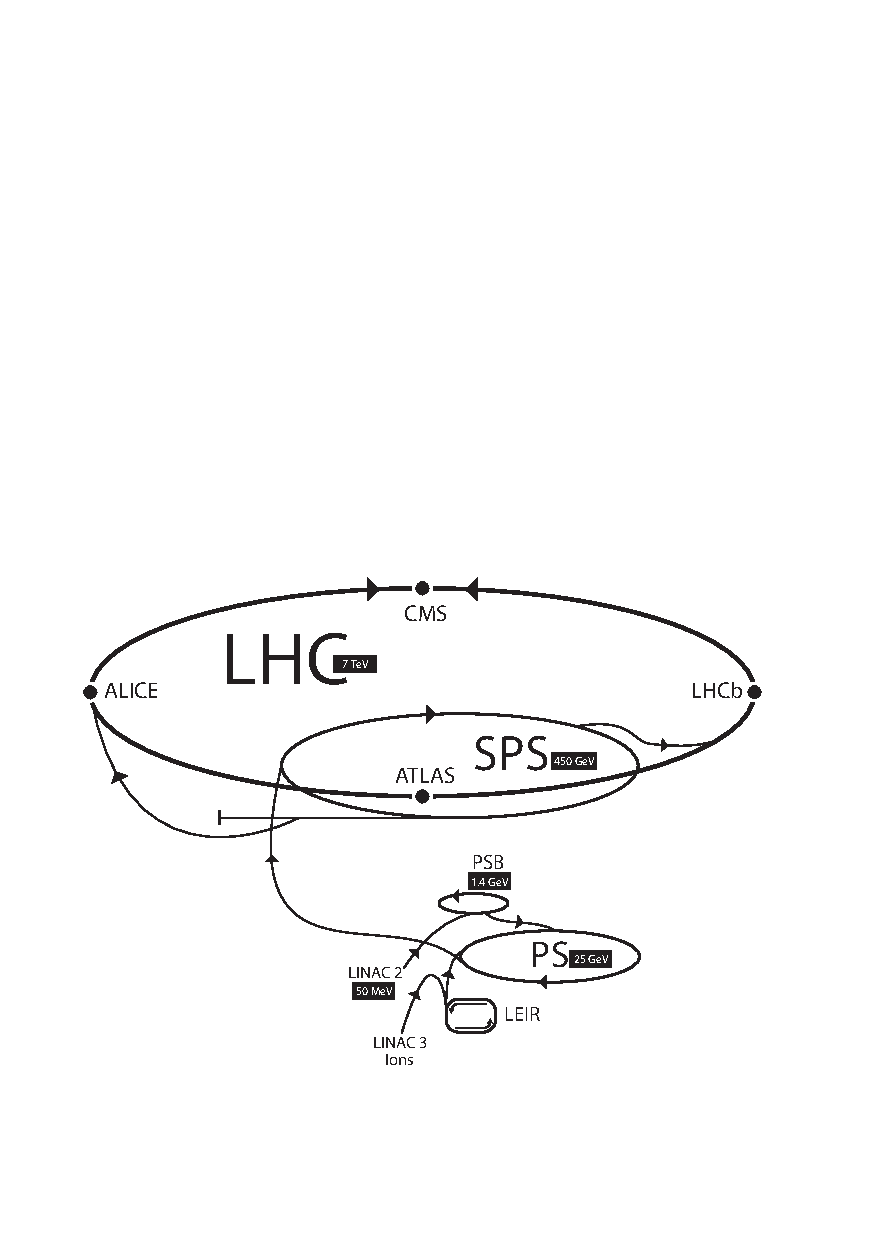
\includegraphics[width=0.48\columnwidth]{chapter3/figs/cern.pdf}
\caption[The \lhc ring.]{A illustration of the the \lhc accelerator complex showing each of the stages in the injection chain 
 for the \lhc ring along with the four main experiments on the \lhc ring~\cite{Lefevre:1092437}. ~\label{fig:lhccomplex} }
\end{figure}
It starts with a linear accelerator which accelerates the protons from rest to 50\mev. 
The synchrotrons increase the beam energy and refine the proton bunches to a configuration suitable for the \lhc. 
Firstly the Proton Synchrotron Booster (PSB) takes the beam from 50\mev to 1.5\gev at which point the 
beam enters the Proton Synchrotron (PS) where the beam energy is increased to 25\gev. 
The beam is then transferred to the Super Proton Synchrotron (SPS) which increases the energy to 450\gev
 before injecting the protons into the \lhc. 
The \lhc accelerates the proton bunches from injection energy at 450\gev to the final collision energy, which was 3.5\tev per beam in 2011 and 4\tev per beam in 2012.
Consolidation upgrades of the \lhc to take place in 2013 and 2014 are expected to increase this collision energy to the design energy of 7\tev per beam.
During operation in 2011-12 there were 1380 proton bunches per beam with a bunch spacing of 50\ns.
There are four main experiments on the \lhc ring, two general purpose detectors (\atlas and \cms), 
along with a heavy-ion experiment (\alice) and a dedicated B-physics experiment (\lhcb).

At the \lhcb interaction point the instantaneous luminosity of the colliding proton bunches 
 is constant at around $\lum\approx3\times10^{32}\cm^2\sec^{-1}$. 
This is significantly below the  \lhc  luminosity, which in 2011 reached over $\lum\approx1\times10^{33}\cm^2\squark^{-1}$.
This luminosity was chosen so that the number of interactions per proton bunch crossing ($\mu$) 
stayed uniform throughout the period of proton collisions for each `fill' of the \lhc.
This ensures that the environment is consistent and has a low multiplicity for reconstruction of \B mesons 
but that there is still a sufficient number of \B meson decays of interest for a given number of collisions.

The production of \bbbar pairs in $pp$ interactions is governed predominantly 
by gluon fusion, $gg\to\bbbar$.
The collision of partons of unequal energy and a momentum boost along the direction of the collision results in \bbbar pairs 
that are produced at small angles to the beam axis.
The angular distribution of \bbbar production is shown in Fig.~\ref{fig:lhcb:bbbar}.
\begin{figure}[tbp]
\centering
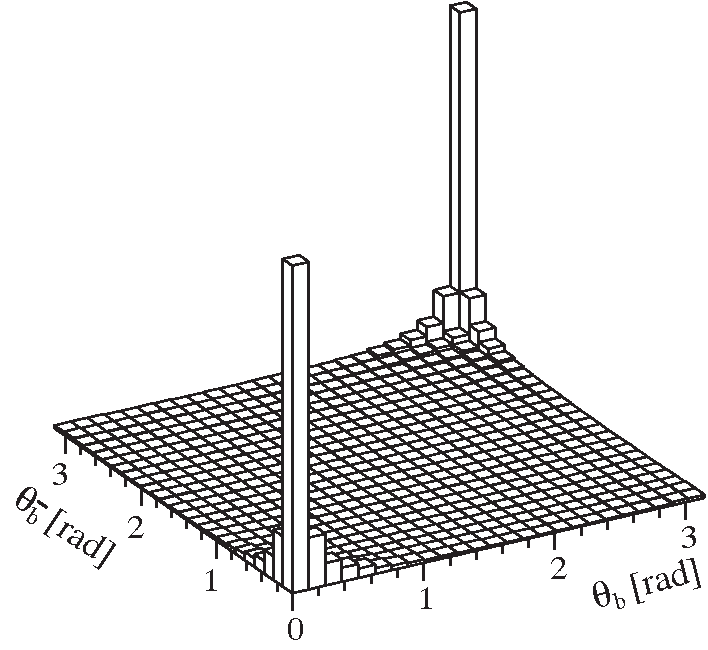
\includegraphics[width=0.48\columnwidth]{chapter3/figs/angular.pdf}
\caption[ $b\bar{b}$ production at the LHC ]{The angular distribution of \bbbar pairs in terms of the polar angle from the beam axis.
The \bbbar pairs are largely produced within a very small opening angle hence the development of \lhcb as a forward spectrometer
~\cite{Alves:2008zz}.~\label{fig:lhcb:bbbar} }
\end{figure}
The \bbbar cross section at \sqs=7\tev is 75\mub within the \lhcb acceptance~\cite{LHCb-PAPER-2010-002}. 
%This corresponds to around $10^7$ \bbbar pairs produced in the 2011 year of data-taking.
In total the experiment recorded an integrated luminosity of 1.0\invfb in 2011 that could be used for further analysis.
The increase in integrated luminosity throughout the year can be seen in Fig.~\ref{fig:lhcb:intlumi} along with the technical stops
 and periods of machine development.
\begin{figure}
\centering
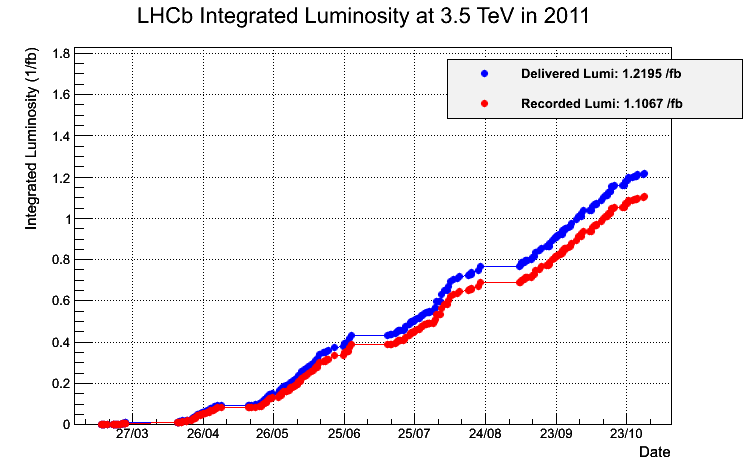
\includegraphics[width=0.66\columnwidth]{chapter3/figs/2011IntegratedLumiLHCbTime_NoPie.png}
\caption{The integrated luminosity recorded by \lhcb during 2011~\cite{OpsPlots}.~\label{fig:lhcb:intlumi} }
\end{figure}


\section{Selection of \BdToKpimm candidates}

\subsection{Data}
\label{sec:swave:meas:data}

The measurement of the S-wave contribution to \BdToKpimm was performed on the complete dataset collected at \lhcb in 2011.
This was the identical dataset used in the second angular analysis presented in Chapter~\ref{chap:kstmm} and 
corresponds to an integrated luminosity of 1.0\invfb at $\sqs=7\tev$. 
The data are described in more detail in Section~\ref{sec:kstmm:data}.

The simulation samples that were used in this measurement consist of the samples already described in Section~\ref{sec:kstmm:data:mc} 
along with an additional sample of \BdToKpimm events.
This additional simulation sample was generated uniformly in phase space and in the MC11 configuration
 using the \lhcb simulation as described in Sec.~\ref{sec:lhcb:soft}.
This simulation was used to understand the efficiency in the wide \kpi mass range.

The data-simulation corrections developed in Sec~\ref{sec:kstmm:data:mccorr} were applied to all of the simulation samples in order to ensure
 that the efficiency calculations were as accurate as possible.



\subsection{Selection}
\label{sec:swave:meas:sel}

The selection of signal \BdToKpimm events was based on the selection presented 
in Section~\ref{sec:kstmm:sel} for \BdToKstmm candidates.
The allowed mass range of \kpi candidates was widened to include the \kpi threshold at $634\mev$ up to $1200\mev$.
This is because there are regions of almost pure S-wave either side of the $\Kstarzo(892)$ as described in Sec~\ref{sec:swave:theo} 
but this range avoids interference from the $\Kstarzt(1430)$.
A cut-based selection was used to remove peaking background events before a multi-variate algorithm
was used to select a pure sample of \BdToKpimm events.

However, this expansion of the \kpi mass window necessitated a 
re-examination of parts of the selection for the angular analysis of \BdToKstmm. 
The vetoes for possible peaking backgrounds, such as the \ktopi swaps and other exclusive \bquark decays,
must also work in the wider \kpi mass window.
In order to select a clean sample of \BdToKpimm candidates, the same multivariate algorithm was 
used to separate potential signal candidates and the remaining combinatorial background.
The selection of \BdToJpsiKpi events was achieved using the same selection but by specifically selecting the \qsq region between 8 and 10 \gevgevcccc
as described in Section~\ref{sec:kstmm:sel}.

\subsection{Peaking backgrounds}

\subsubsection{\ktopi swaps}

Candidates which cannot be separated through hadron identification are called \ktopi swaps because they pass the selection 
with reasonable kaon and pion identification when  the kaon and pion masses are swapped.
These `swaps' manifest as duplicate candidates and require vetoing to avoid double counting.
These \ktopi swaps were vetoed in Section~\ref{sec:kstmm:sel} under two conditions. 
The invariant mass of the \kpi pair with the pion and kaon masses exchanged must have fallen in the \kpi window
and the hadron identification values must have satisfied the condition that the difference between the \dllkpi for the kaon (\kdllkpi) and the pion (\pidllkpi) was greater than minus ten.
However, this condition fails to veto sufficient candidates in the wide \kpi window. 

The distribution of \ktopi swaps in terms of \kdllkpi and \pidllkpi for selected \BdToKpimm candidates
is given in Fig.~\ref{fig:swave:meas:kpiswaps}. 
\begin{figure}[tbp]
\centering
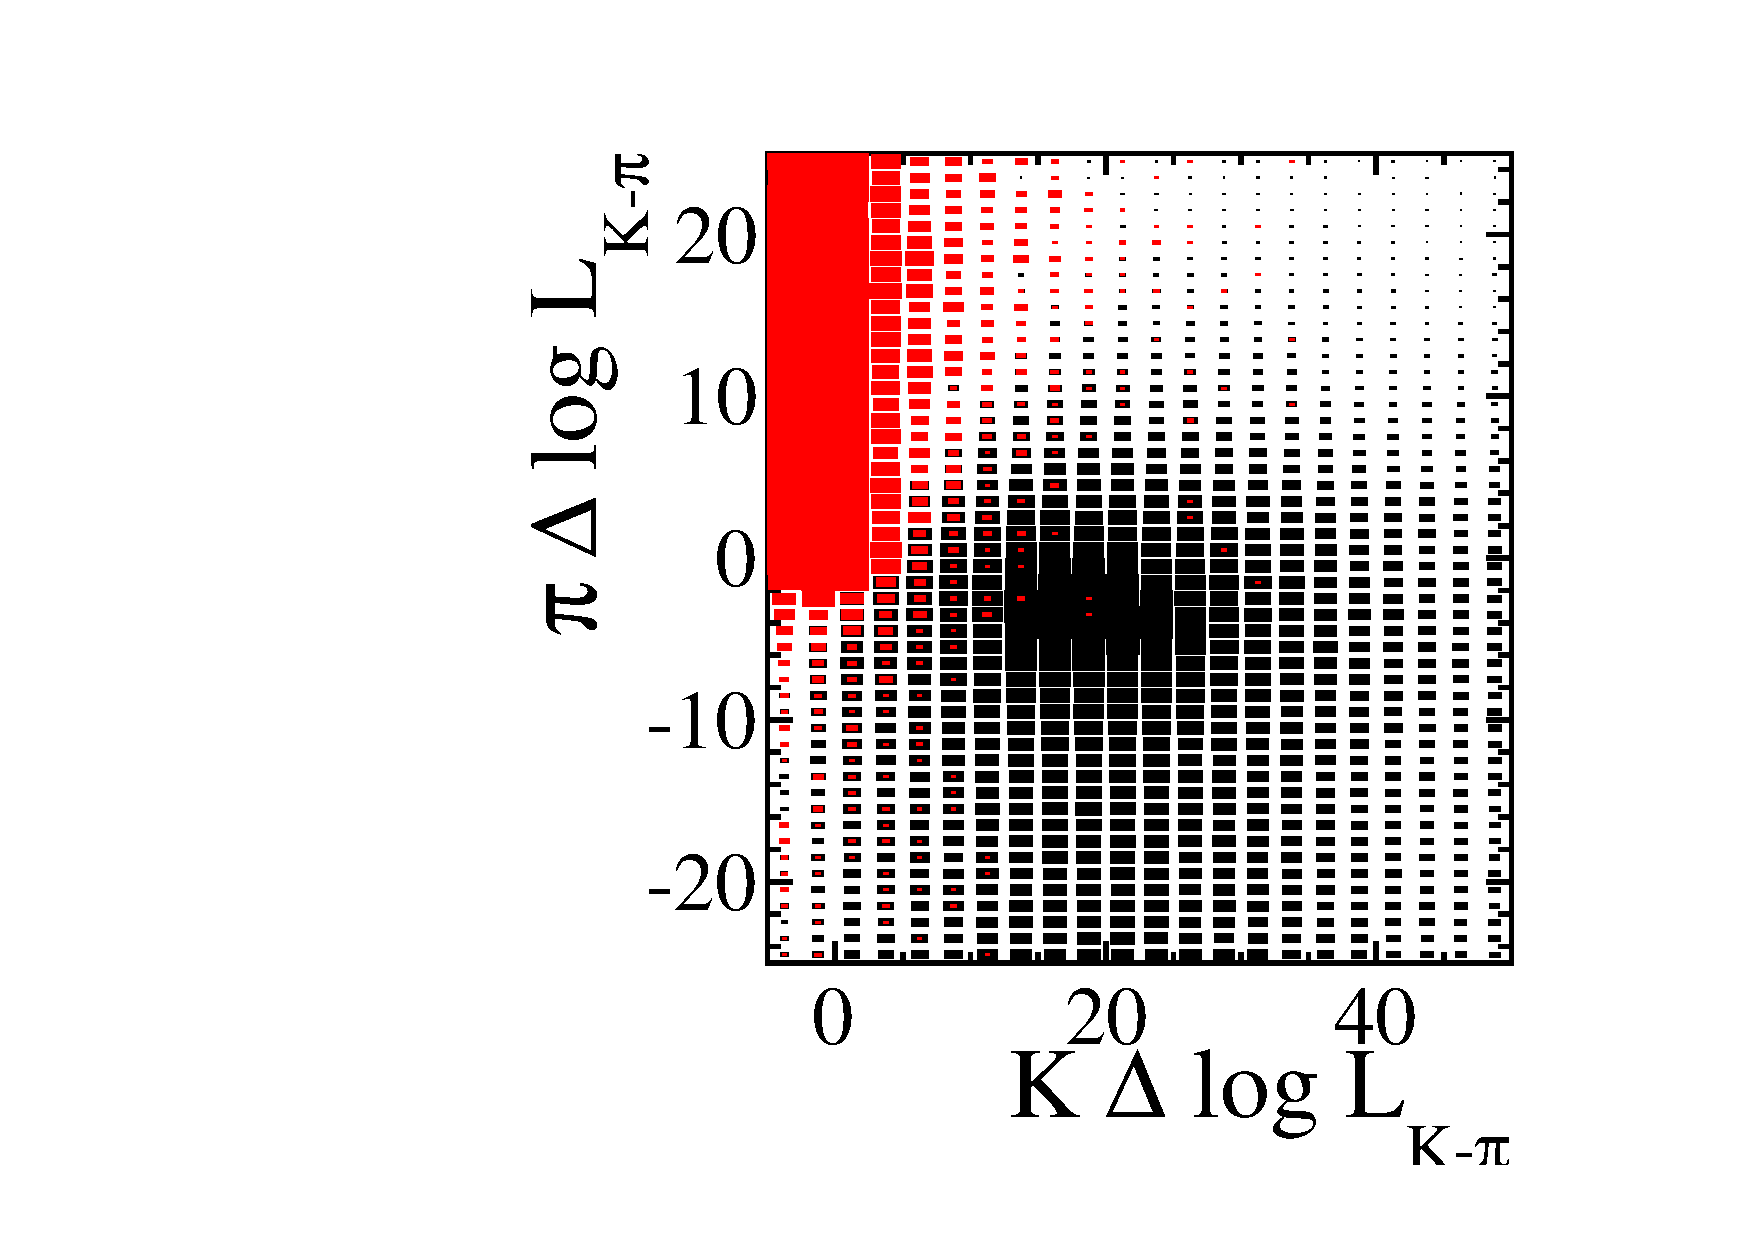
\includegraphics[width=0.48\columnwidth]{chapter7/figs/kstarmumu_swap_2Ddist.pdf}
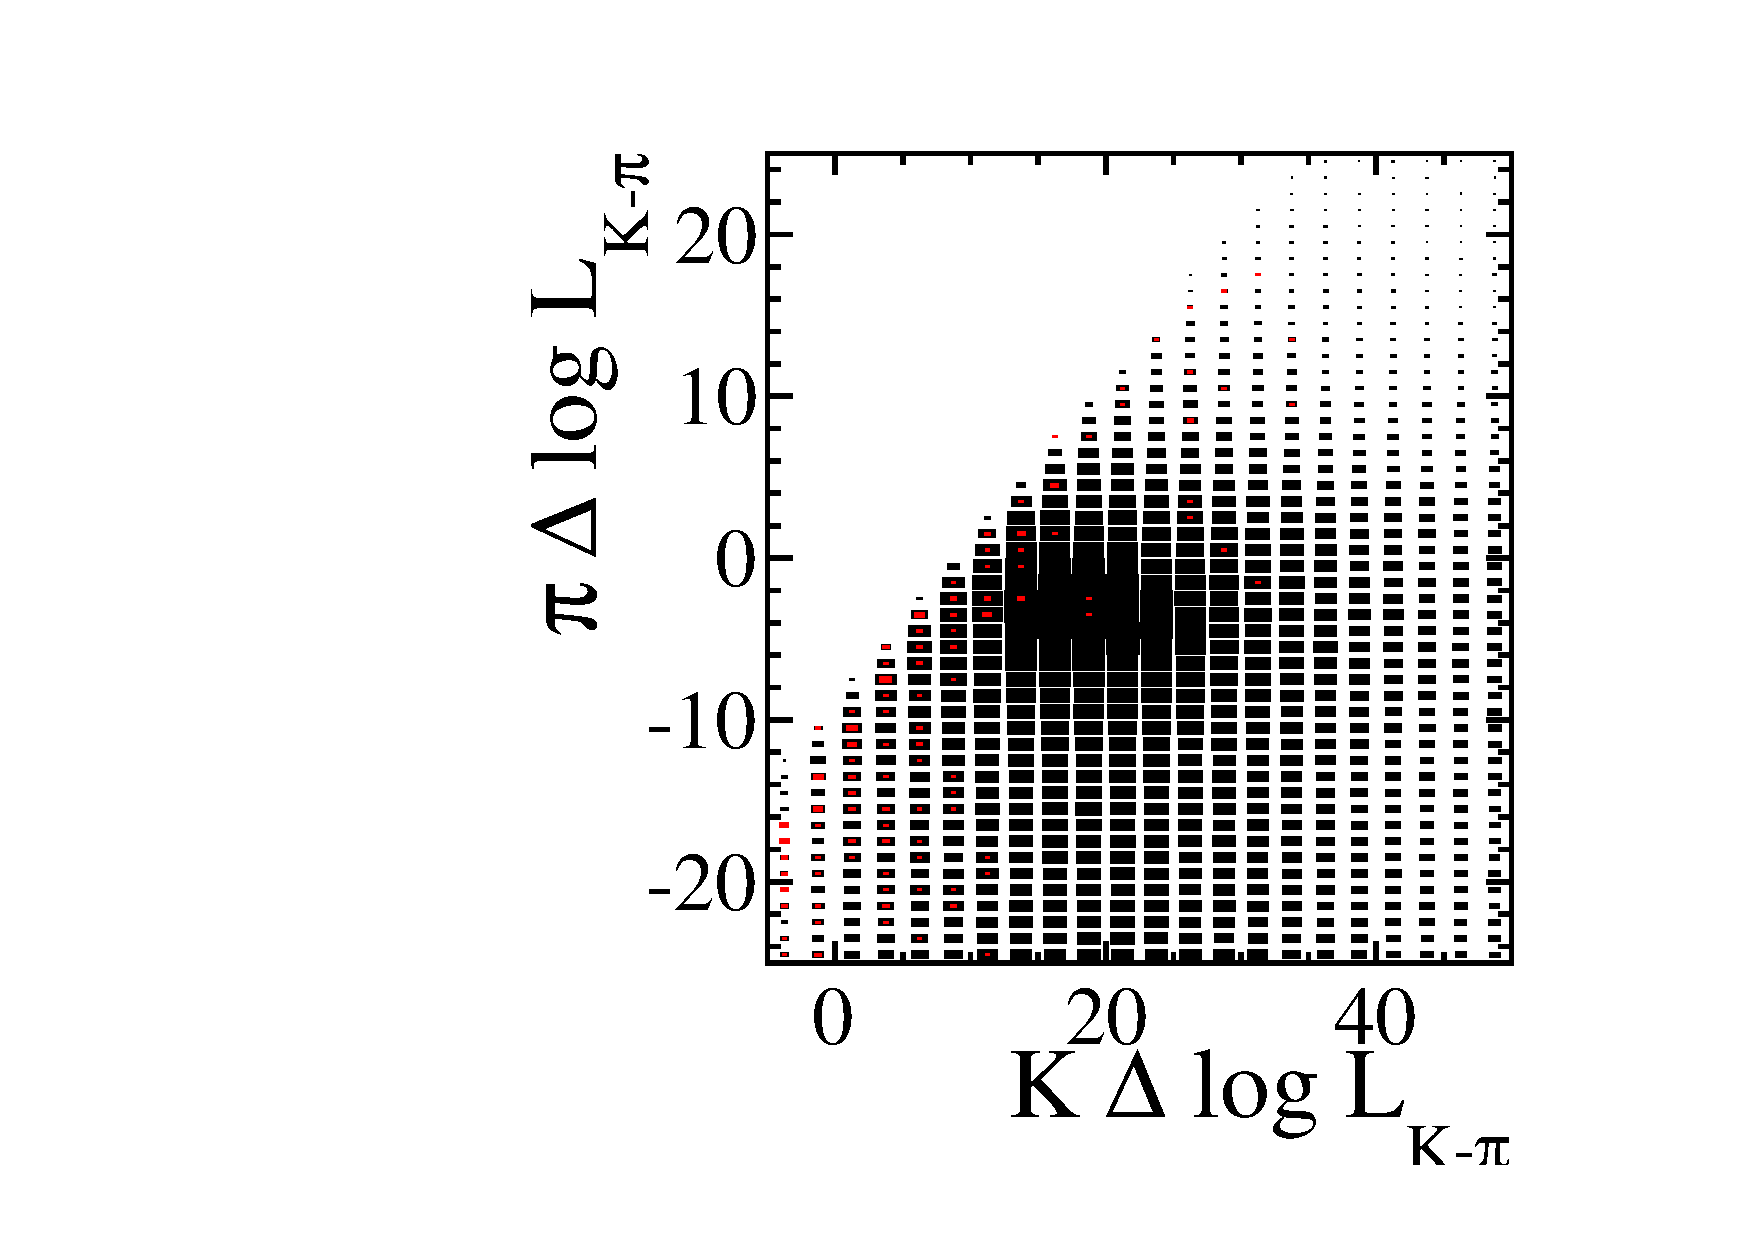
\includegraphics[width=0.48\columnwidth]{chapter7/figs/kstarmumu_swap_2Ddist_veto.pdf}
\caption[  The distribution of \BdToKpimm simulation (a) before and (b) after the \ktopi swap veto.   ]
{The distribution of \BdToKpimm simulation (a) before and (b) after the \ktopi swap veto. 
Candidates with the correction assignment of masses for the kaon and pion are shown in black and candidates 
with the incorrect assignment of masses are shown in red. There is a clear overlap of candidates around \dllkpi of 0 for both particles.
~\label{fig:swave:meas:kpiswaps} }
\end{figure}
The overlap of the two distributions can be seen around the zero point motivating the use of the diagonal cut, $\kdllkpi-\pidllkpi>10$.
The efficiency of the swap veto is around 92\% on signal events which pass the multivariate selection and 
less than 2.5\% of swapped candidates are retained after the veto.
There are less than 0.1\% of \ktopi swap candidates in the simulation after selection.

\subsubsection{Other peaking backgrounds}

The possible sources of peaking backgrounds considered have a % are also considered in Section~\ref{sec:kstmm:sel} and
mass close to the \Bd mass after the misidentification of one or more of the final state particles
 and could create structure in the \kpi mass spectrum. They are
\begin{itemize}
\item \BdToKstmm with the pion misidentified as the muon and the muon as the pion.
\item \BdToKstmm with the kaon misidentified as the muon and the muon as the kaon.
\item \BsToPhimm with one of the kaons misidentified as a pion.
\item \BuToKmm with an added soft pion.
\item \LbToLmm (1) with the proton misidentified as a pion.
\item \LbToLmm (2) with the proton misidentified as a kaon and the kaon misidentified as a pion.
\end{itemize}
In order to understand the \kpi mass distribution of these exclusive backgrounds, 
simulation samples for each decay were used. % generated and corrected as described in Section~\ref{sec:kstmm:data:mccorr} .
Each simulation sample was weighted so that the number of events in the sample was equivalent to the expected yield from 1.0\invfb of data.
The number of events after selection for the signal \Bd and \kpi mass region, the signal \Bd and the wide \kpi mass region
 and the wide \Bd and the wide \kpi mass region are shown in Table~\ref{tbl:peaking:backgrounds}.
\begin{table}
\centering
\caption[   The expected number of peaking background events from selected simulated data in three different mass ranges
for an integrated luminosity of 1.0\invfb.   ]
{ The expected number of peaking background events from selected simulated data in three different mass ranges
for an integrated luminosity of 1.0\invfb. The assumed branching fraction is given in the first column.
The first mass range is from $5230<\mB<5330\mevcc$ and $800<\mkpi<1000\mevcc$. 
The second mass range is from $5230<\mB<5330\mevcc$ and $634<\mkpi<1200\mevcc$ 
The third range mass range is from $5200<\mB<5700\mevcc$, $634<\mkpi<1200\mevcc$. 
The errors are statistical.~\label{tbl:peaking:backgrounds} }
\begin{tabular}{|c|c|c|c|c|}
\hline
Background  & $\Gamma$  & Range 1 & Range 2 & Range 3 \\
\hline
\BdToKstmm ( $K\leftrightarrow\pi$ )  &   $1.0\times10^{7}$&  $ 0.119\pm0.345 $ &$ 0.158\pm0.397 $ &$ 0.487\pm0.698 $ \\ 
\BdToKstmm ( $\pi\leftrightarrow\mu$ )  & $1.0\times10^{7}$&  $ 0.5\pm0.707 $ &$ 1.5\pm1.22 $ &$ 2.33\pm1.53 $ \\ 
\BdToKstmm ( $K\leftrightarrow\mu$ ) &    $1.0\times10^{7}$&  $ 0\pm0 $ &$ 0\pm0 $ &$ 0\pm0 $ \\ 
\BsToPhimm  &                             $5.5\times10^{7}$&  $ 3.1\pm1.76 $ &   $ 5.93\pm2.44 $ &$ 7.91\pm2.81 $ \\ 
\BuToKmm  &                               $6.0\times10^{7}$&  $ 0.0851\pm0.292 $ &  $ 0.17\pm0.413 $ &$ 1.3\pm1.14 $ \\ 
\LbToLmm (1)  &                           $1.0\times10^{7}$&  $ 13.2\pm4.63 $ &   $ 25.1\pm7.01 $ &$ 79.7\pm10.93 $ \\ 
\LbToLmm (2) &                            $1.0\times10^{7}$&  $ 3.8\pm2.95 $ &$ 6.82\pm3.61 $ &$ 13.3\pm5.64 $ \\  
\hline
\end{tabular}
\end{table}
%As measured in Section~\ref{sec:kstmm:res}, there are 900 \BdToKstmm candidates in the 1.0\invfb data. 
%This means that most of the peaking backgrounds are around 1\% or less in the signal region, 
%justifying their ignorance in the previous measurement.
%However, there are larger contributions from the peaking backgrounds in the high \kpi mass region and the higher \Bd mass region.
The distribution of peaking background simulation is given in figure~\ref{fig:swave:peaking:backgrounds}.
\begin{figure}
\centering
\subfigure[]{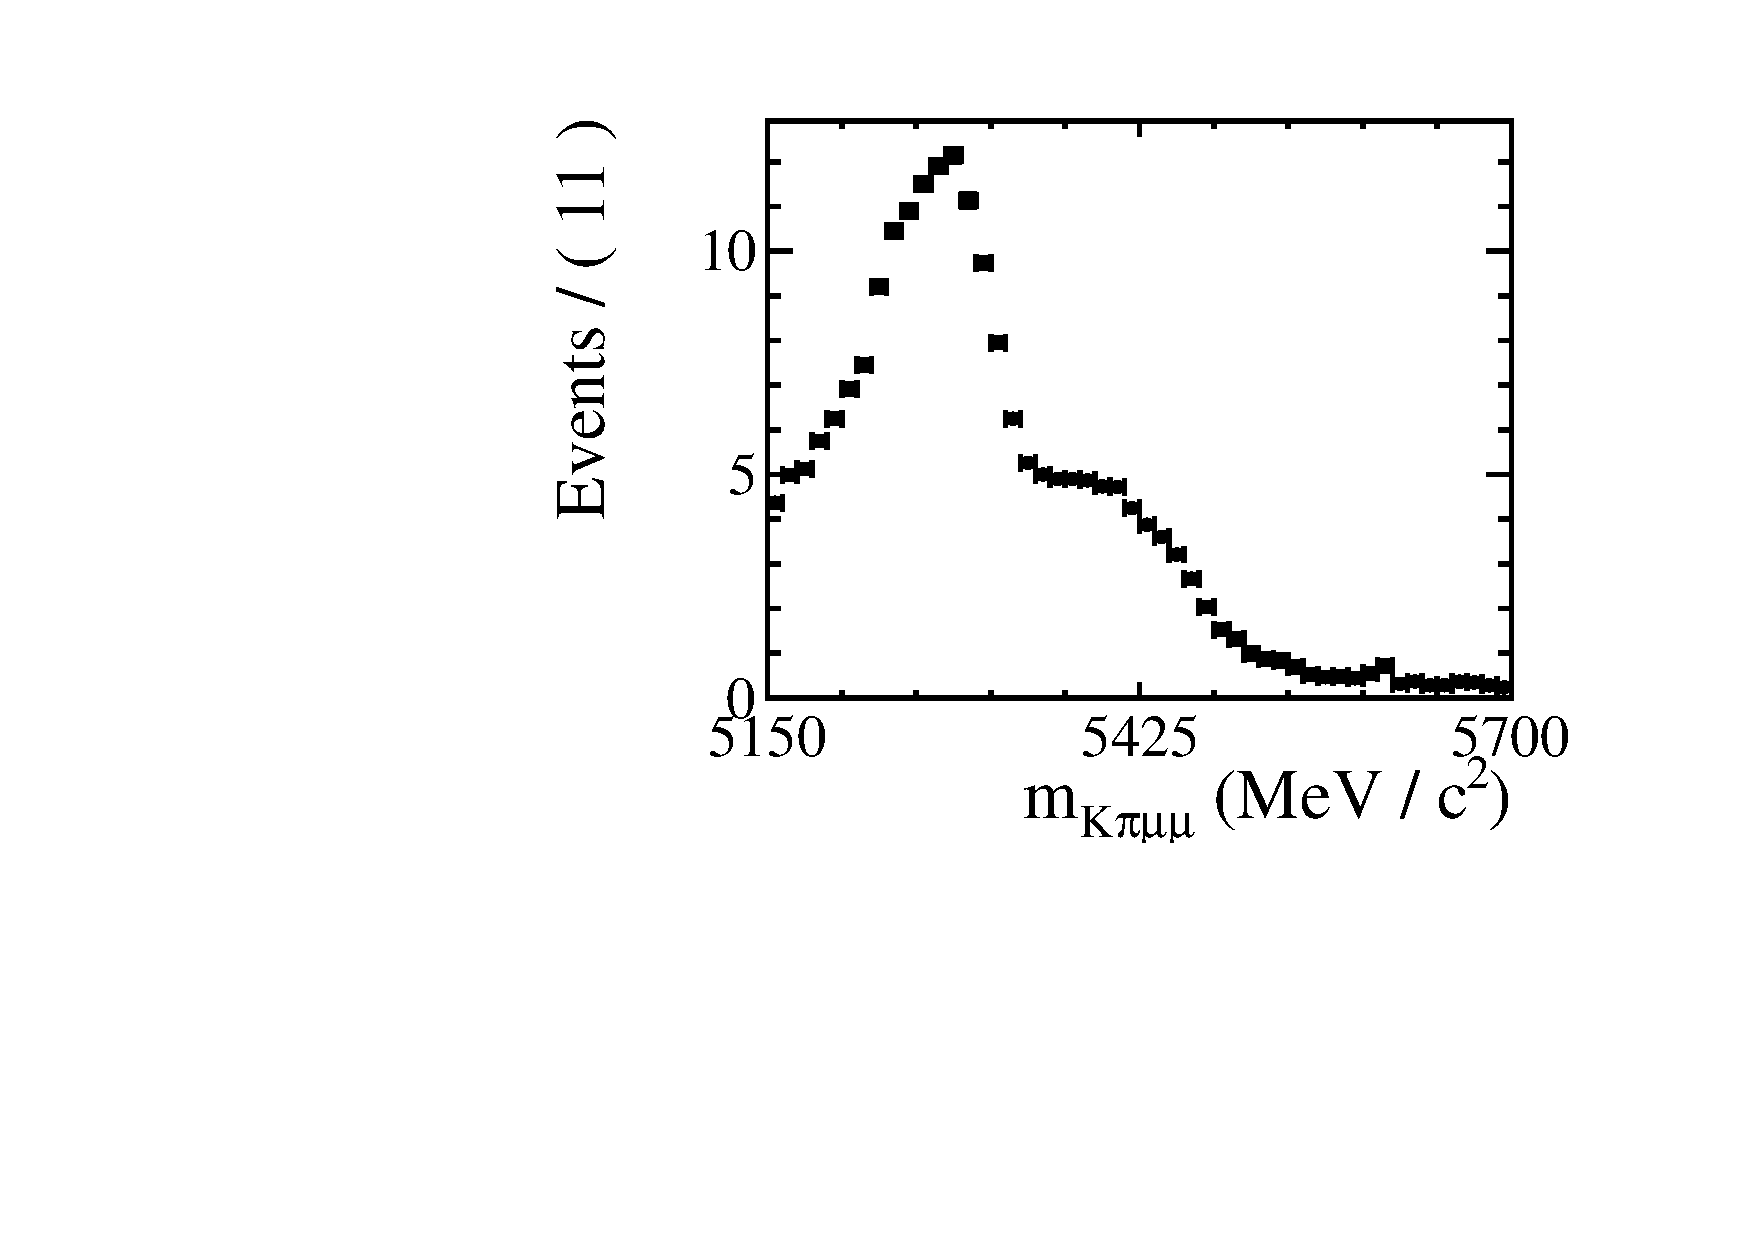
\includegraphics[width=0.32\columnwidth]{chapter7/figs/peaking/peaking_backgrounds_mass.pdf}}
\subfigure[]{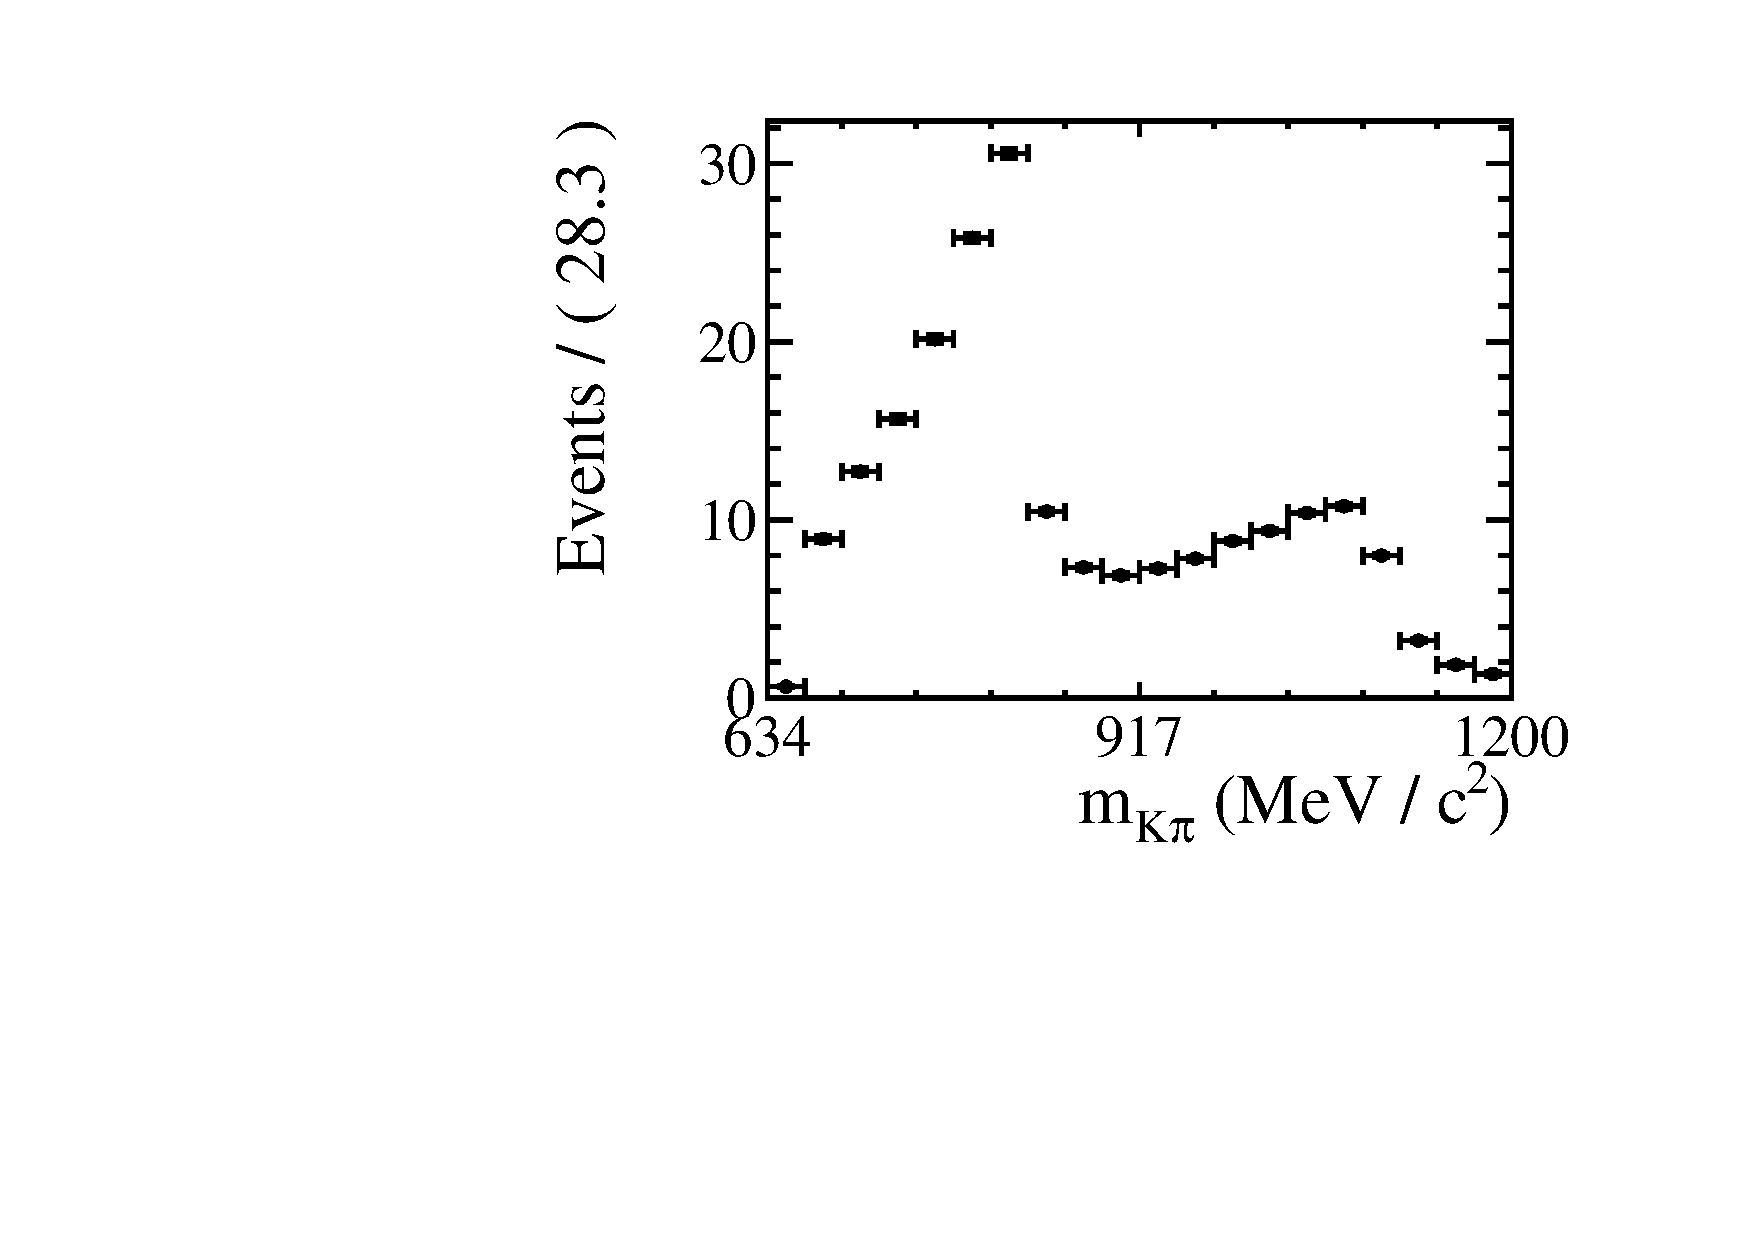
\includegraphics[width=0.32\columnwidth]{chapter7/figs/peaking/peaking_backgrounds_mkpi.pdf}}
\subfigure[]{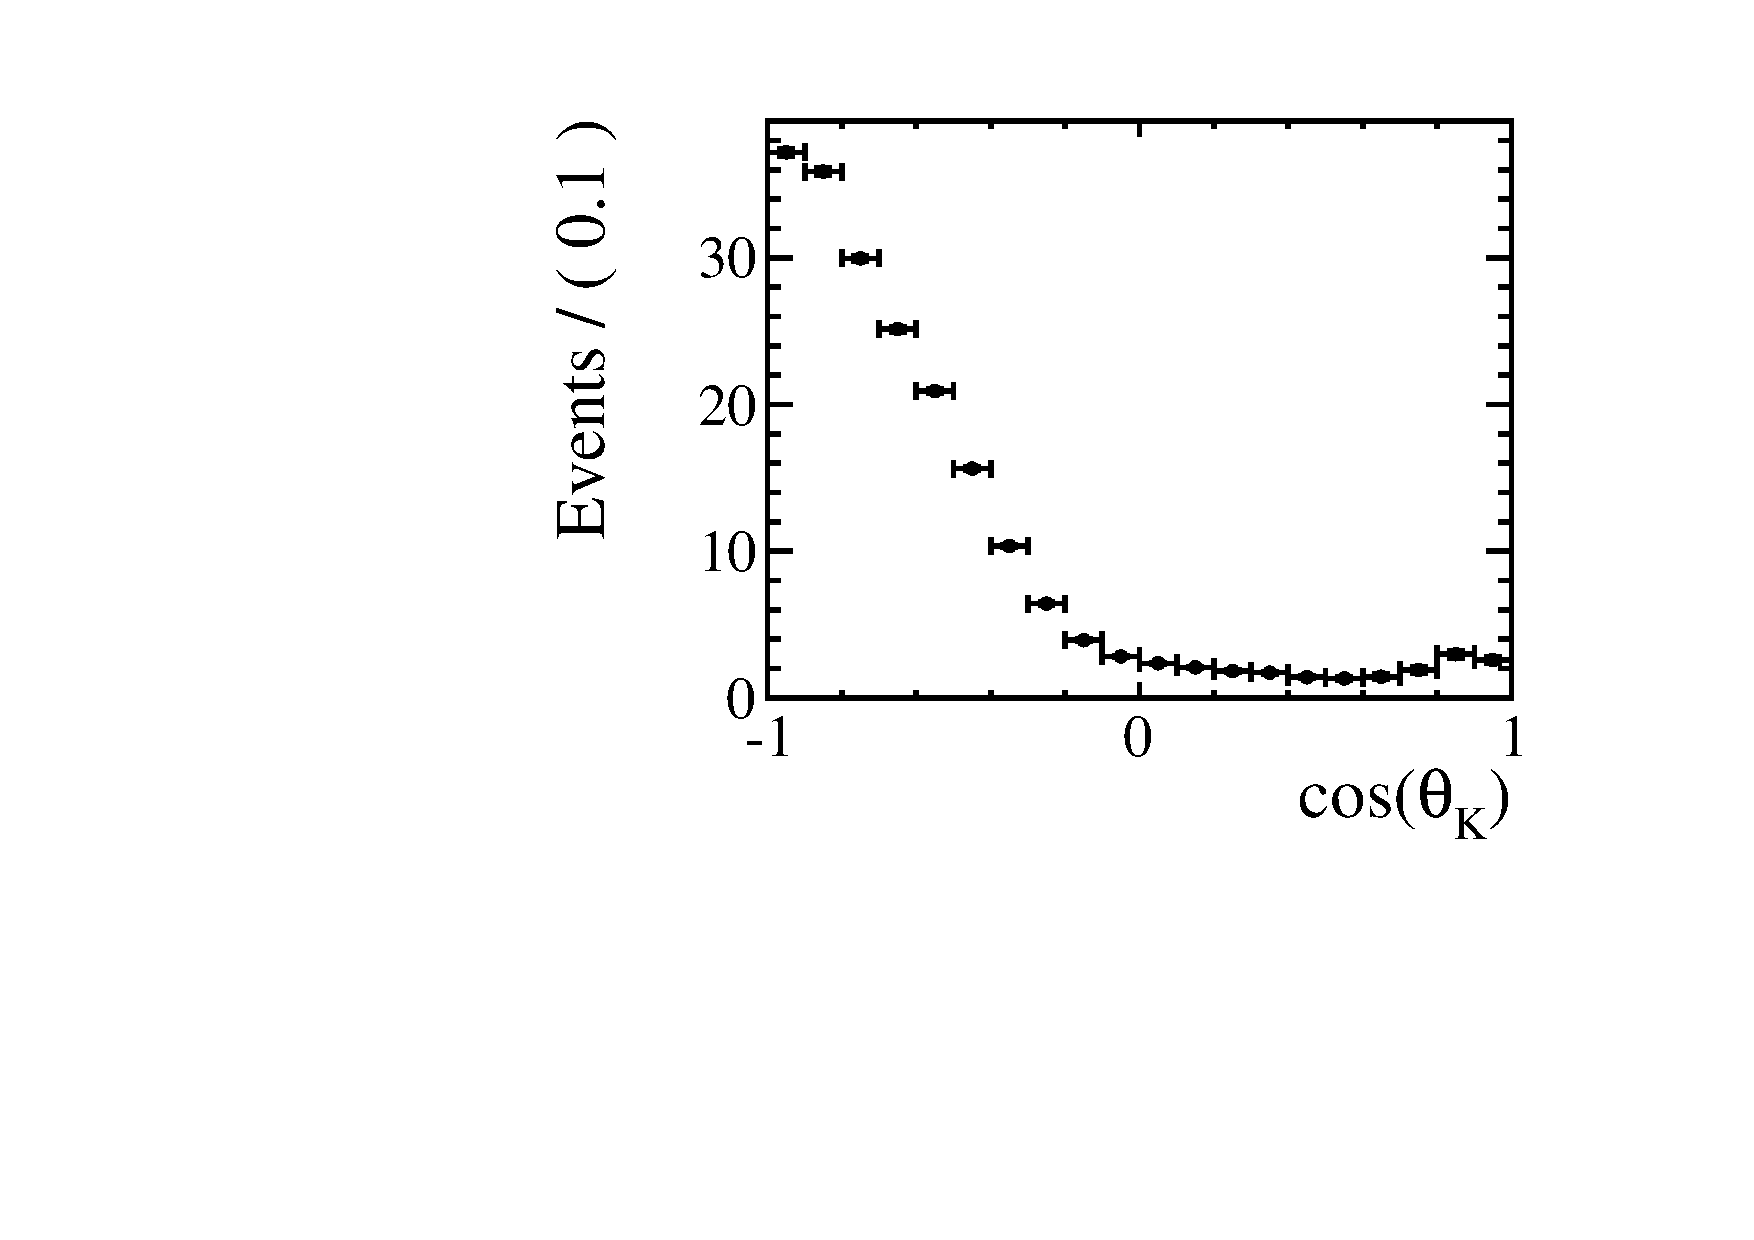
\includegraphics[width=0.32\columnwidth]{chapter7/figs/peaking/peaking_backgrounds_ctk.pdf}}
\caption[ The combined distribution of peaking background events after selection in terms of (a) \mkpimm, (b) \mkpi and (c) \ctk.   ]
{ The combined distribution of peaking background events after selection in terms of (a) \mkpimm, (b) \mkpi and (c) \ctk.
The distribution is composed of simulated \BdToKstmm, \BsToPhimm, \BuToKmm and \LbToLmm normalised to
the expected number of events in 1.0\invfb of data. %It is possible to see non-trivial shapes 
%in the \kpimm and \kpi mass distributions.% but the number of events is almost insignificant.
~\label{fig:swave:peaking:backgrounds} }
\end{figure}
It is possible to see structure in each of the \mkpill, \mkpi and \ctk distributions.
However, the fraction of peaking background events in the \kpill mass window is less than $(2.0\pm0.2)\%$ after the selection allowing these contributions to be ignored under the P-wave peak.

%\subsection{Data distributions}
%The distribution of selected \BdToKpimm and \BdToJpsiKpi candidates as a function of \mB and \mkpi are shown in Fig.~\ref{fig:swave:mass:mkpi}.
%Here the \mkpi window is extended upwards to 2000\mev to show the overall distribution of events at high \mkpi.
%\begin{figure}[tbp]
%\centering
%\subfigure[]{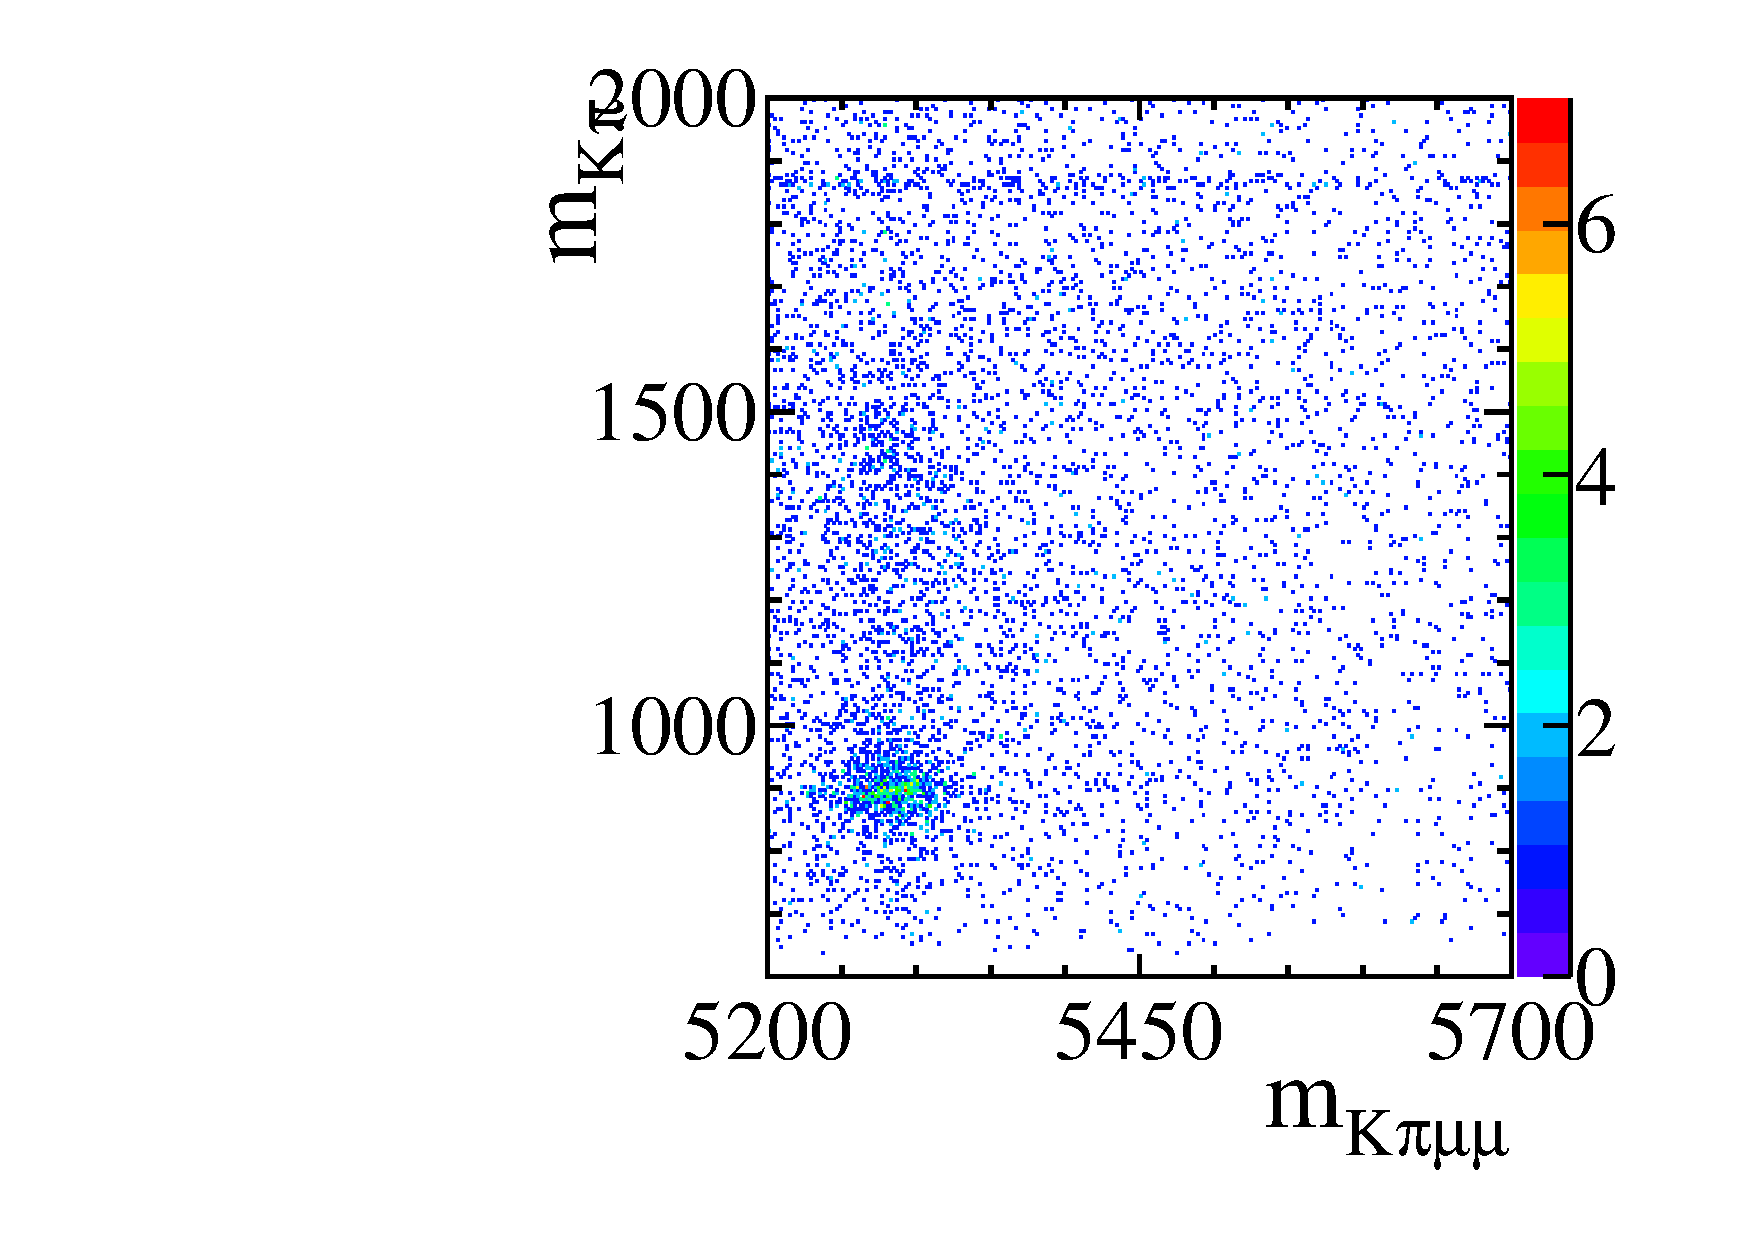
\includegraphics[width=0.48\columnwidth]{chapter7/figs/massdists_kstarmumu_mB_mkpi.pdf}}
%\subfigure[]{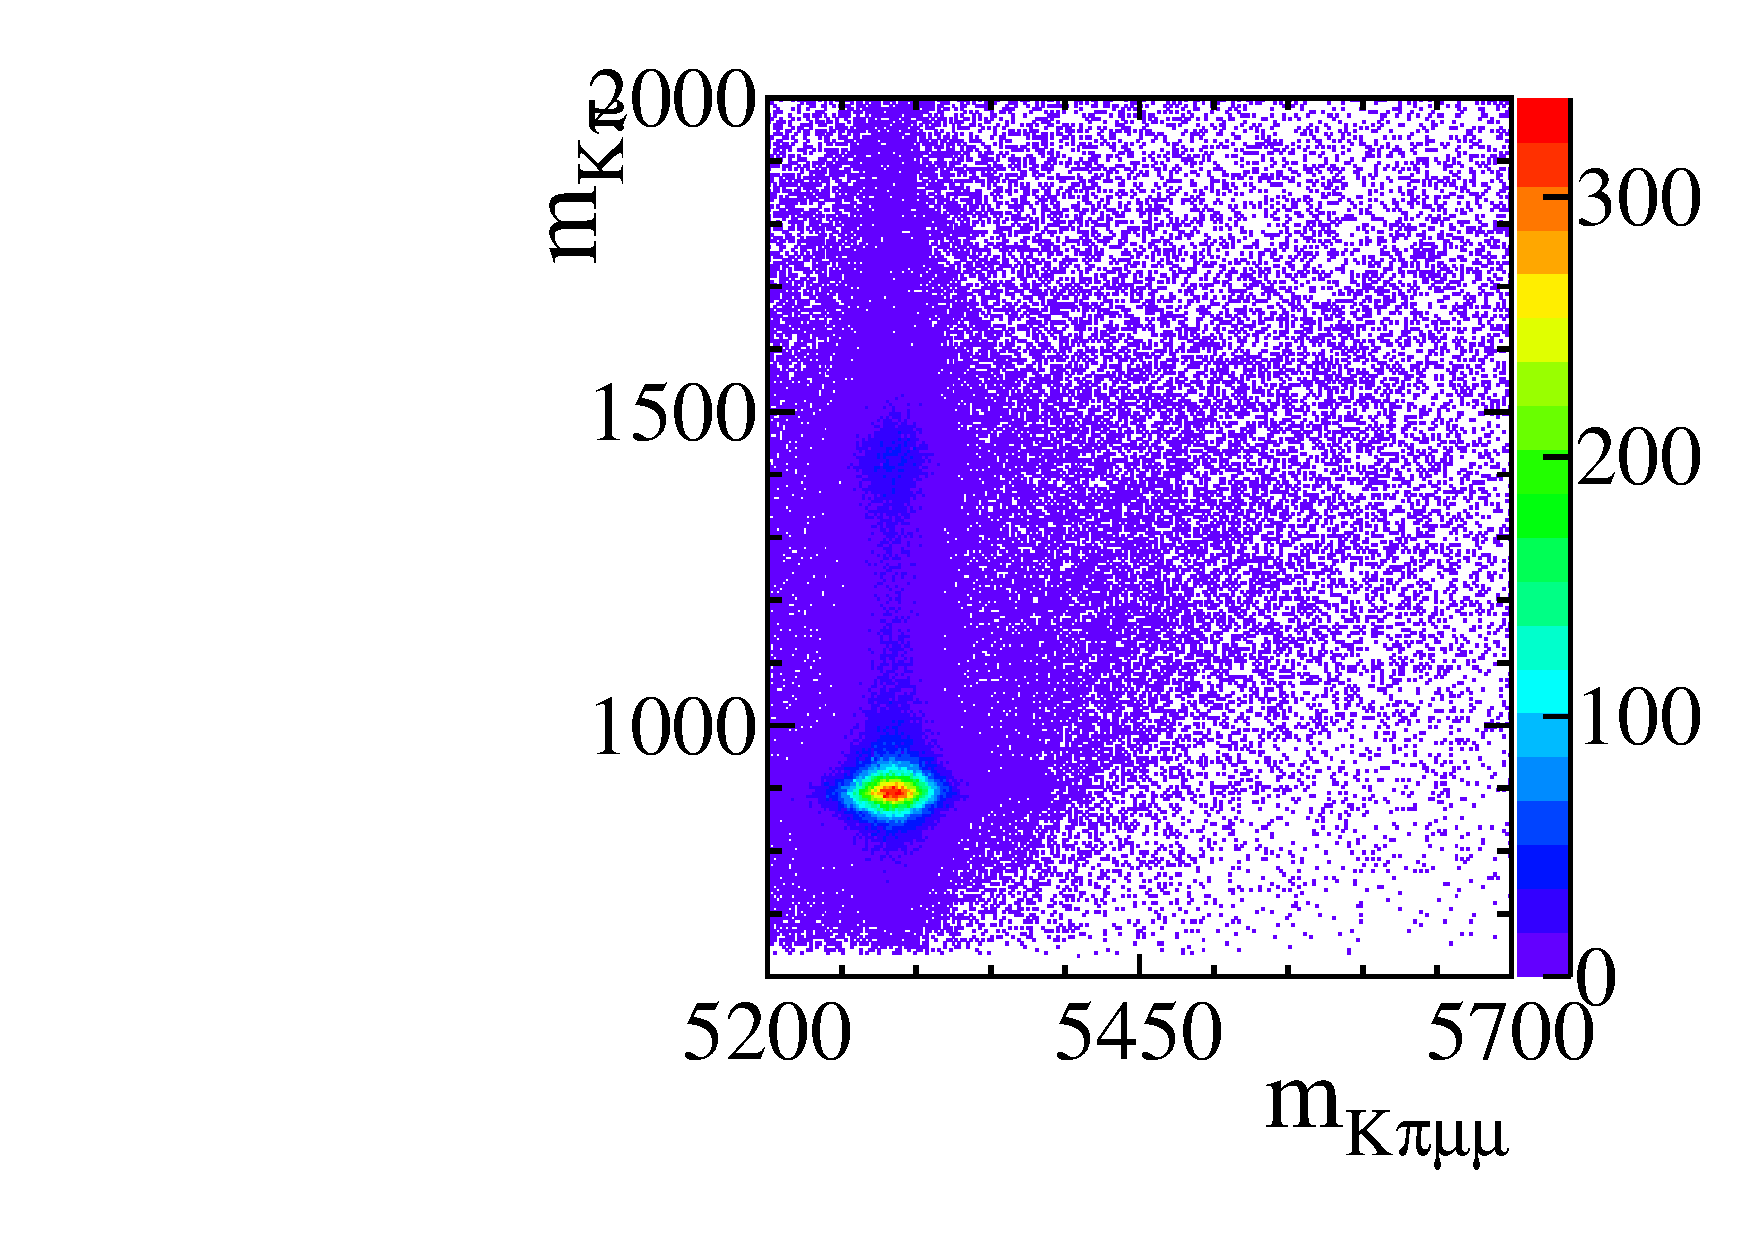
\includegraphics[width=0.48\columnwidth]{chapter7/figs/massdists_jpsikstar_mB_mkpi.pdf}}
%\caption{ \mB v.s. \mkpi mass distributions for the wide \mkpi region for (a) \BdToKstmm and (b) \BdToJpsiKstar. 
%In the \BdToKstmm selection, it is possible to see the P-wave clearly and a 
%combinatorial background from \D \mumu at $\mkpi\sim1800$.
%In the \BdToJpsiKstar selection, is it possible to see both the P-wave, the \kpi S-wave and a \Kstarz D-wave at 1430.
%There is also an asymmetric background in \mkpi and \mB. ~\label{fig:swave:mass:mkpi} }
%\end{figure}
%It is possible to see a clear peak of \BdToKstmm events along with a generic S-wave and 
%contributions from the $\Kstarzt(1430)$ in the \BdToJpsiKpi spectrum as described in Ref~\cite{LHCB-PAPER-2012-014}.
%There is significant difference between the high \mB background between \BdToJpsiKpi and \BdToKpimm.
%The background for the charmonium mode can be seen in increase with \mkpi indicating that it is mis-reconstructed physics background whereas the 
% \BdToKpimm background is constant as a function of \mkpi indicating that it is composed of mostly combinatorial background.






\section{Acceptance correction}
\label{sec:kstmm:ac}

The angular distribution of fully reconstructed and offline selected \BdToKstmm candidates 
is not representative of the angular distribution of \BdToKstmm events
which come from a proton-proton interaction.
This is because the process of reconstruction and selection introduces an acceptance
effect, both from the geometry of the \lhcb detector and from the reconstruction and selection
software. 
In order to perform an angular analysis, this acceptance effect must be corrected for.
There are two main approaches to including the acceptance in an angular analysis.
The acceptance can be parametrised and included in the signal \PDF and fitted to the data,
along with various external inputs to help constrain the parameters.
This approach has several benefits but it also introduces additional parameters into the fit.
Angular analyses that have used this approach include the \lhcb and \cdf measurements of $\Bd\to\jpsi\phi$~\cite{CDF:2011af,Aaij:1407836}.
As an alternative, the efficiency can be calculated in different regions of phase space to give each candidate a
weight proportional to the inverse of the efficiency,
\begin{align}
\omega(\ctl,\ctk,\phi)_i = \frac{1}{ \epsilon(\ctl,\ctk,\phi)_i } \, .
\end{align}
This method has the benefit of being separate from the result extraction, keeping the angular \PDF purely to describe the data. 
This is the method presented in this thesis and was the method used in the first two angular analyses of \BdToKstmm at \lhcb.

\subsection{Total acceptance effect on simulation}
\label{sec:kstmm:ac:effect}

Simulation was used to calculate the selection efficiency for \BdToKstmm candidates in different regions of phase space
by comparing the distribution of \BdToKstmm candidates as a function of the angular variables and \qsq
 before and after the complete selection has been applied.
The simulated events were generated as described in Section~\ref{sec:lhcb:soft} 
and corrected as described in Section~\ref{sec:kstmm:data:mccorr}.
The IP resolution and the particle identification corrections were applied before the selection. 
The distribution of the weights given to each of the simulated \BdToKstmm 
 candidates from the remaining data-simulation corrections is shown in Fig~\ref{fig:datamc:weight}.
\begin{figure}[tbp]
\centering
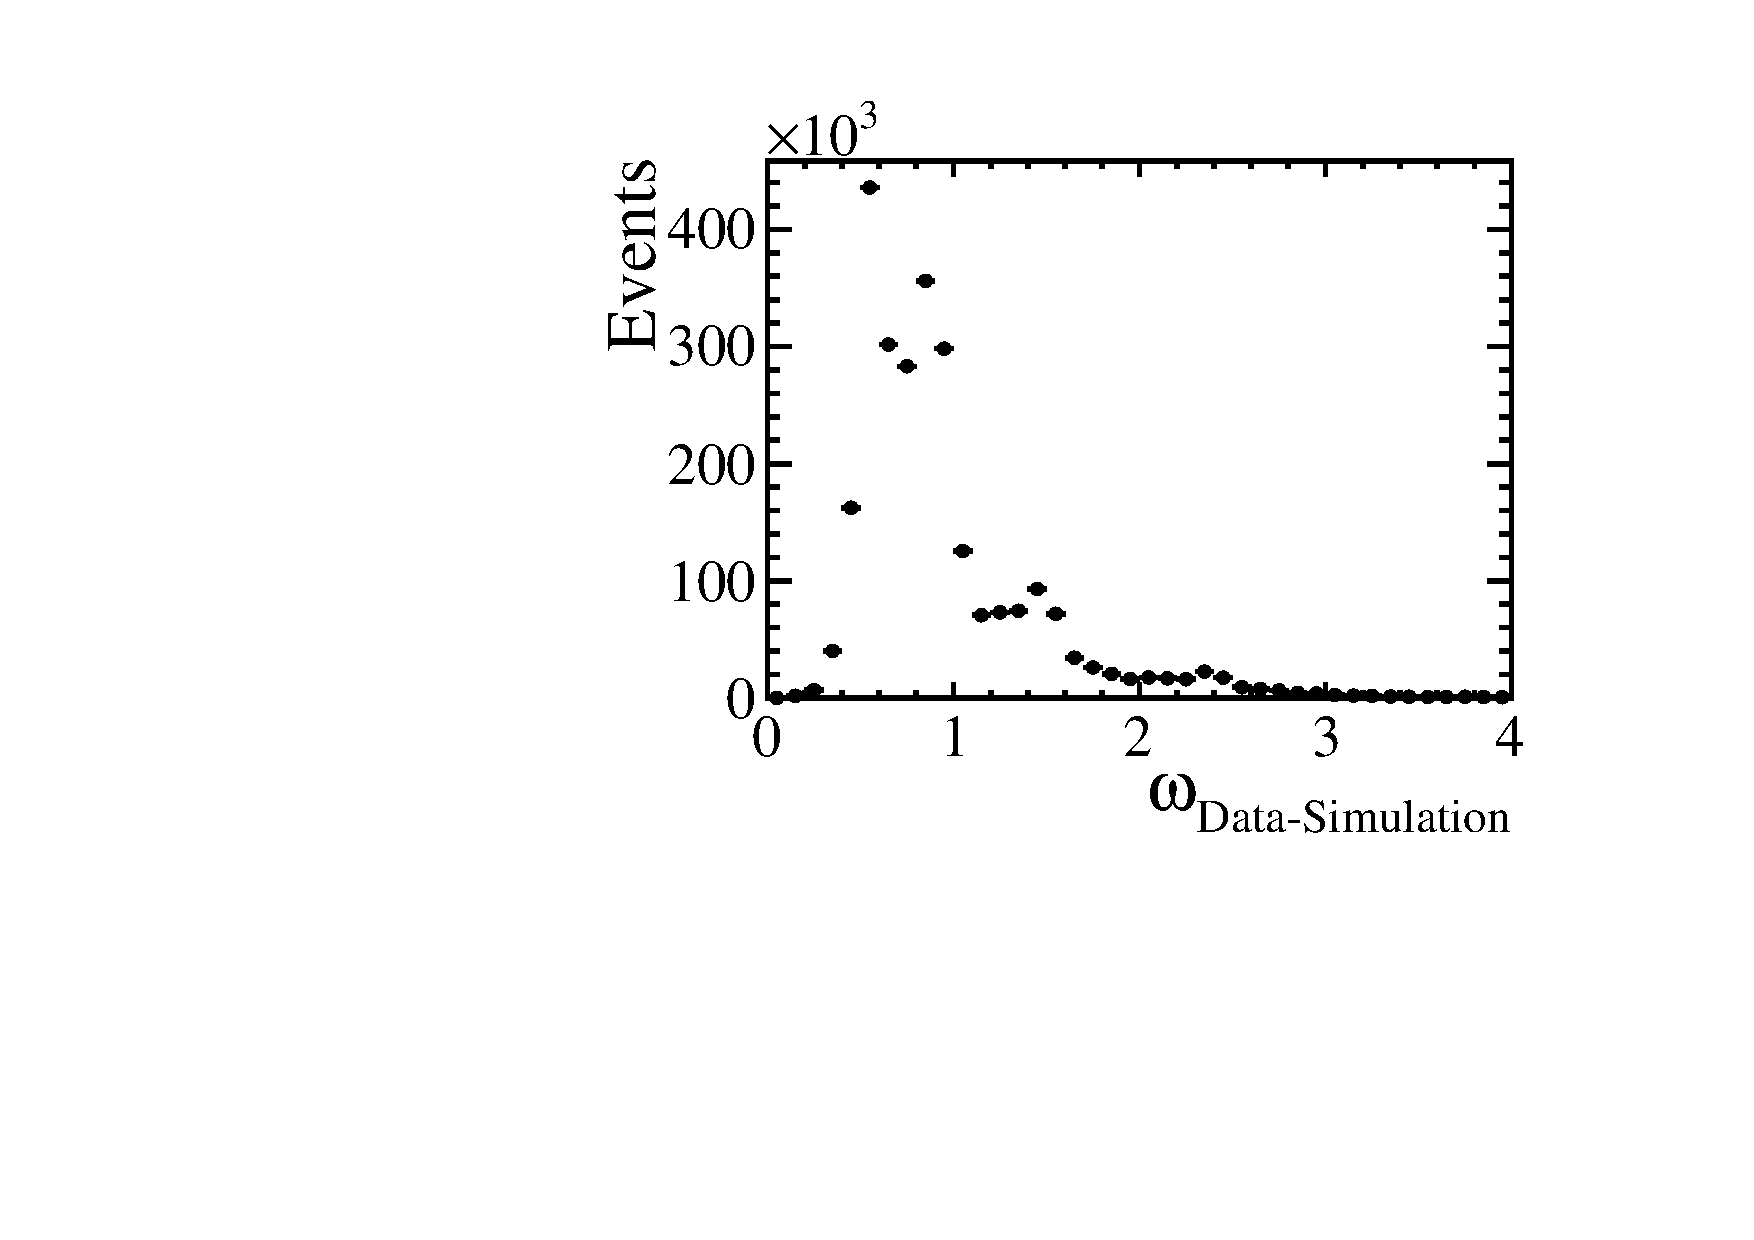
\includegraphics[width=0.48\columnwidth]{chapter5/figs/datamc/datamc_jpsikstar.pdf}
\caption{The distribution of weights to correct the simulated phase space \BdToKstmm candidates
 for known differences between the data and the simulation. ~\label{fig:datamc:weight} }
\end{figure}
The structure of four distinct peaks comes from the re-weighting for the event occupancy.

The angular distribution of fully reconstructed and selected phase space \BdToKstmm candidates
is given in Fig.~\ref{fig:phspeff}. 
\begin{figure}[tbp]
\centering
\subfigure[]{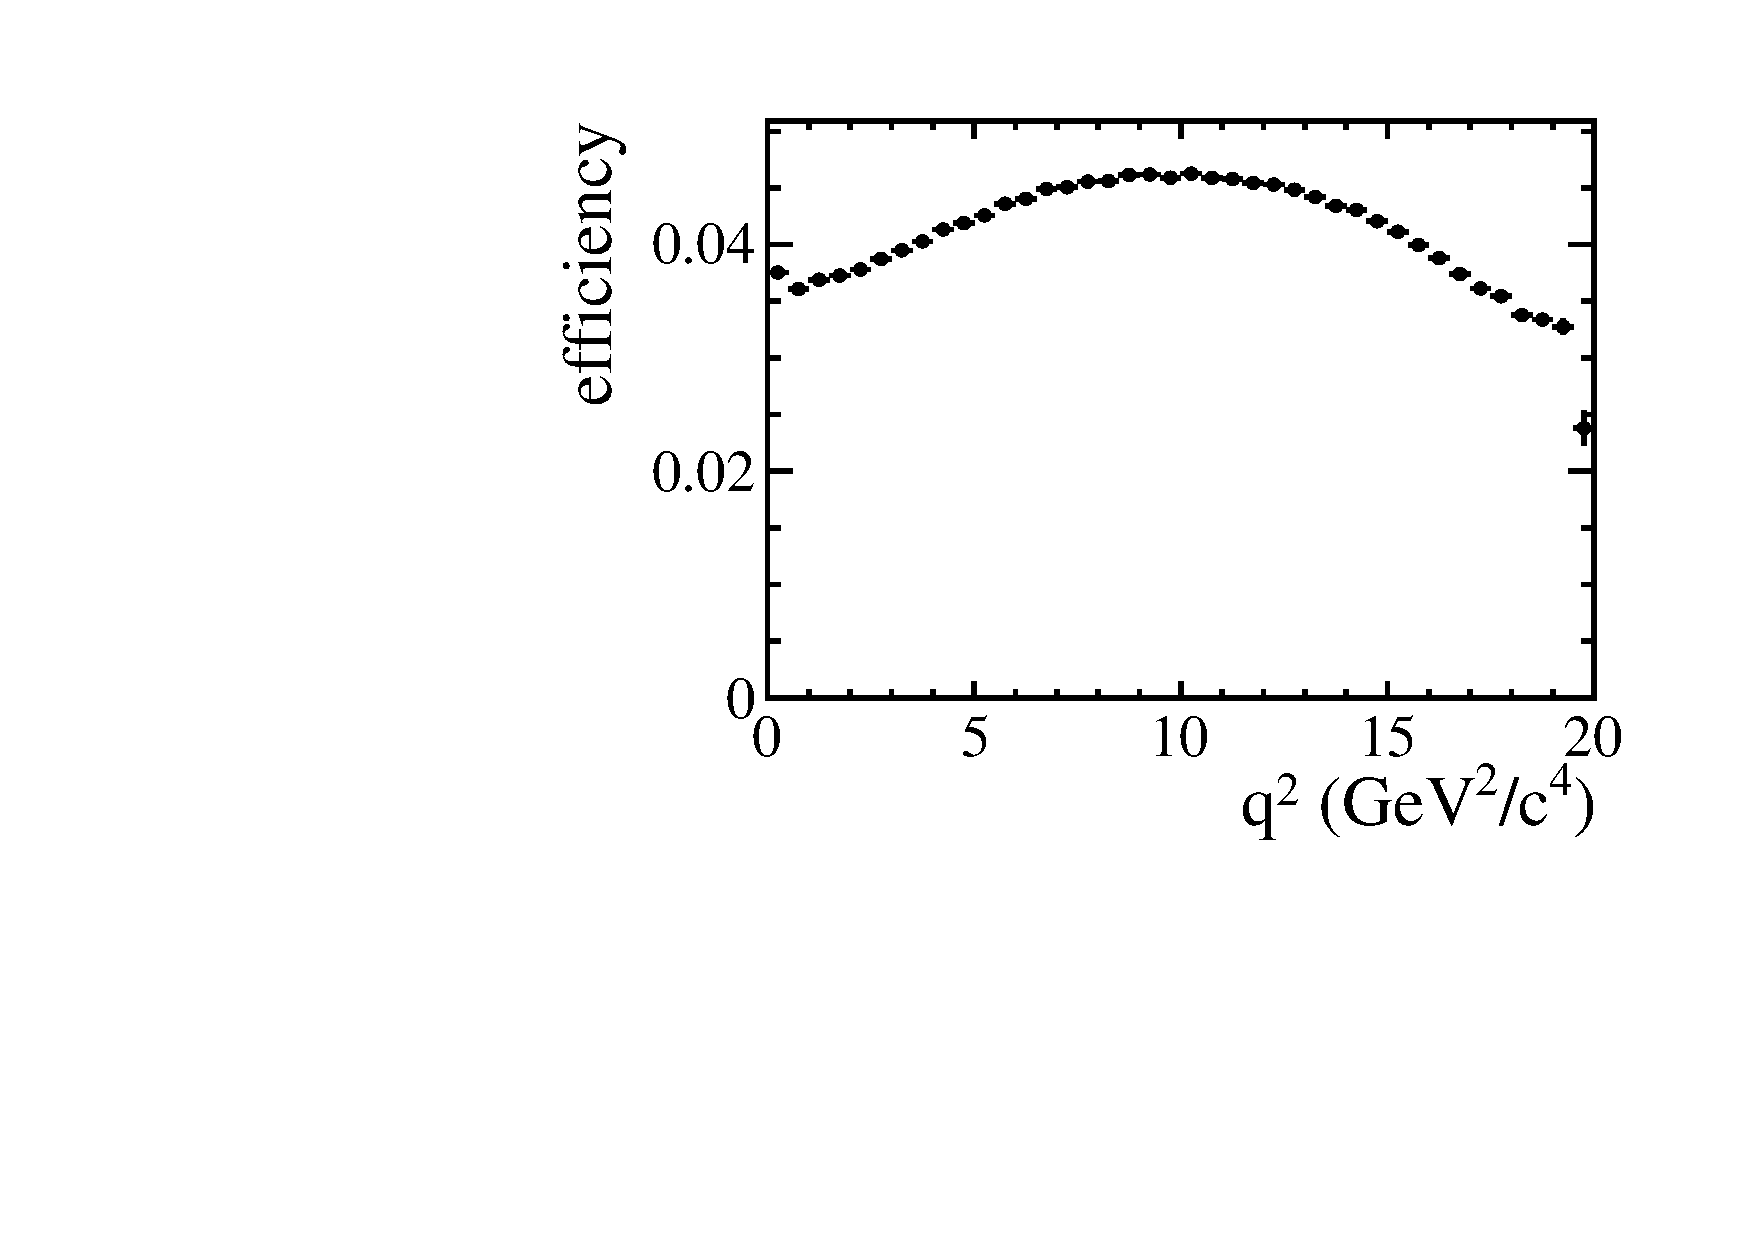
\includegraphics[width=0.48\columnwidth]{chapter5/figs/phsp_qsq_eff_dist.pdf}}
\subfigure[]{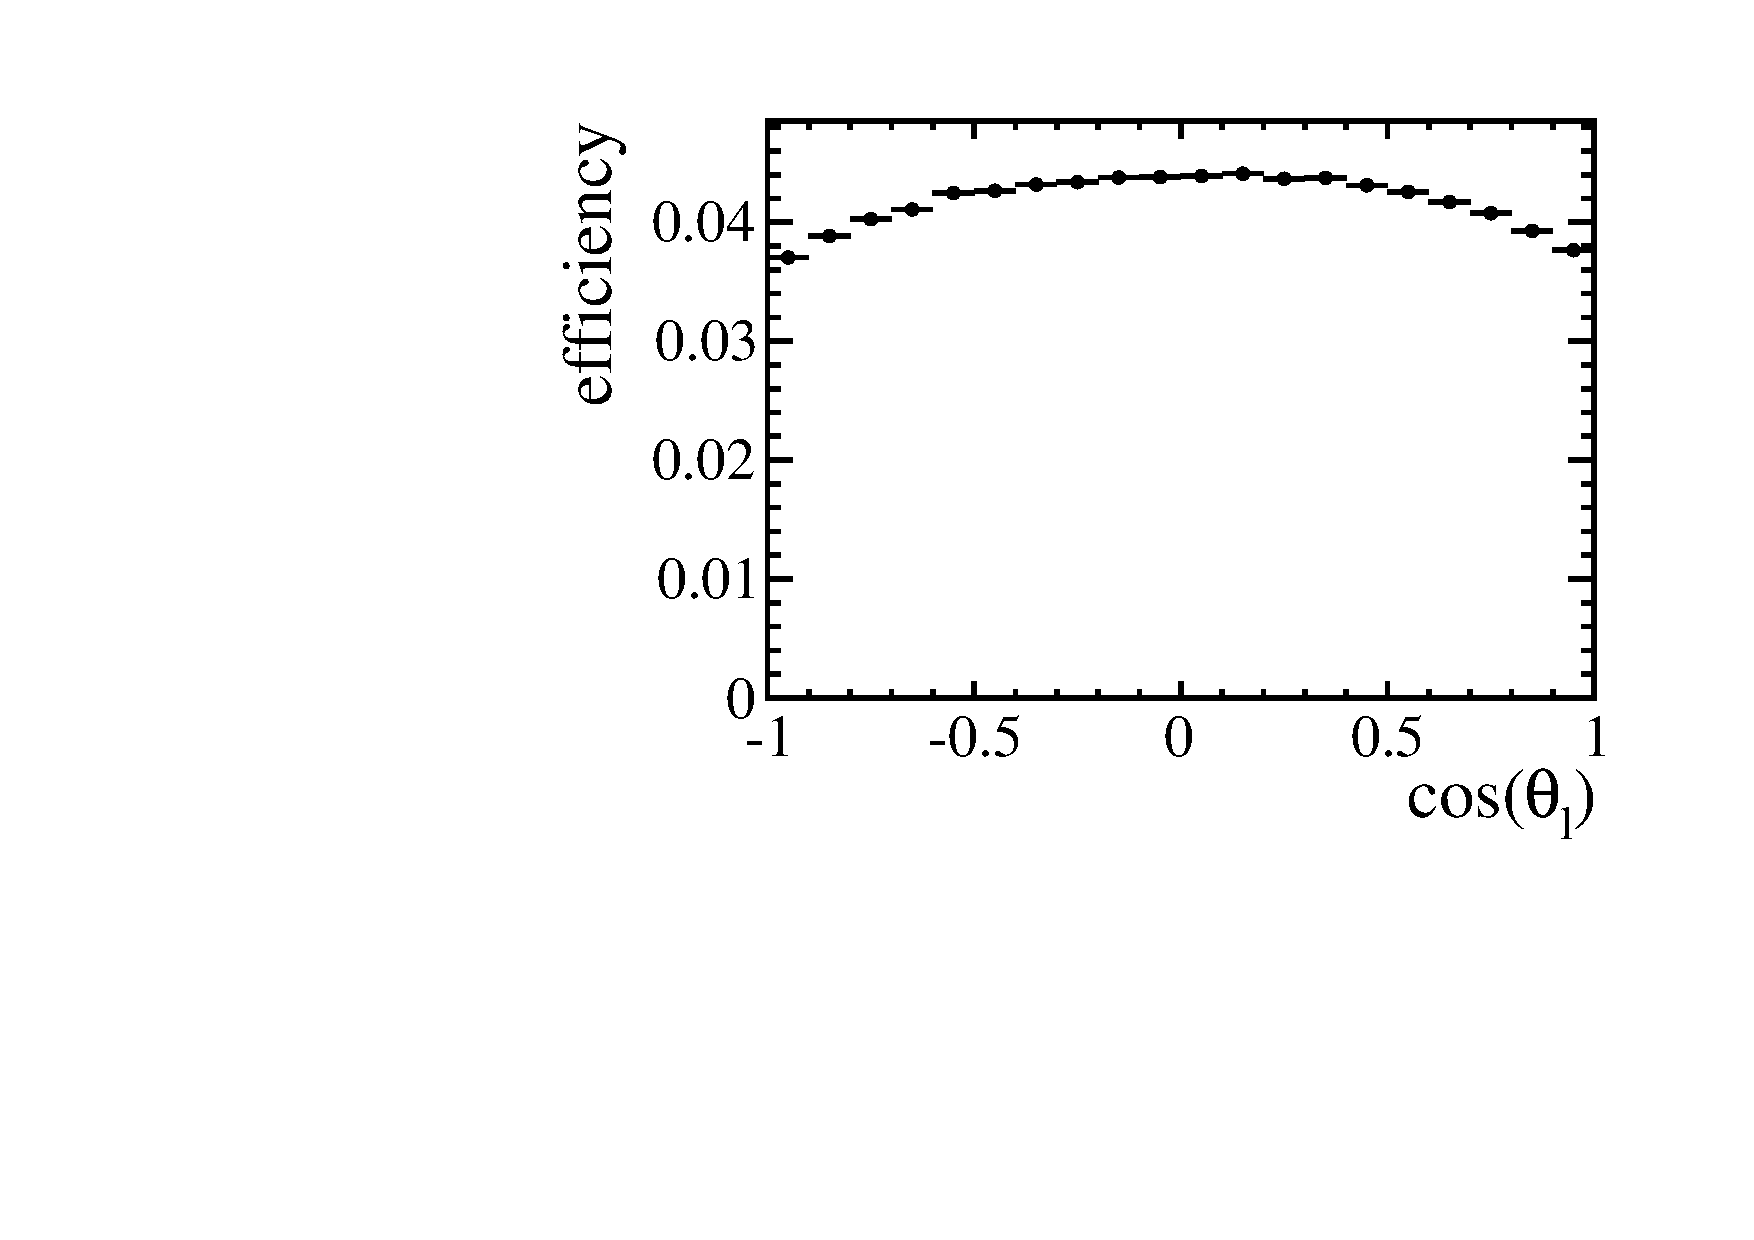
\includegraphics[width=0.48\columnwidth]{chapter5/figs/phsp_ctl_eff_dist.pdf}}
\subfigure[]{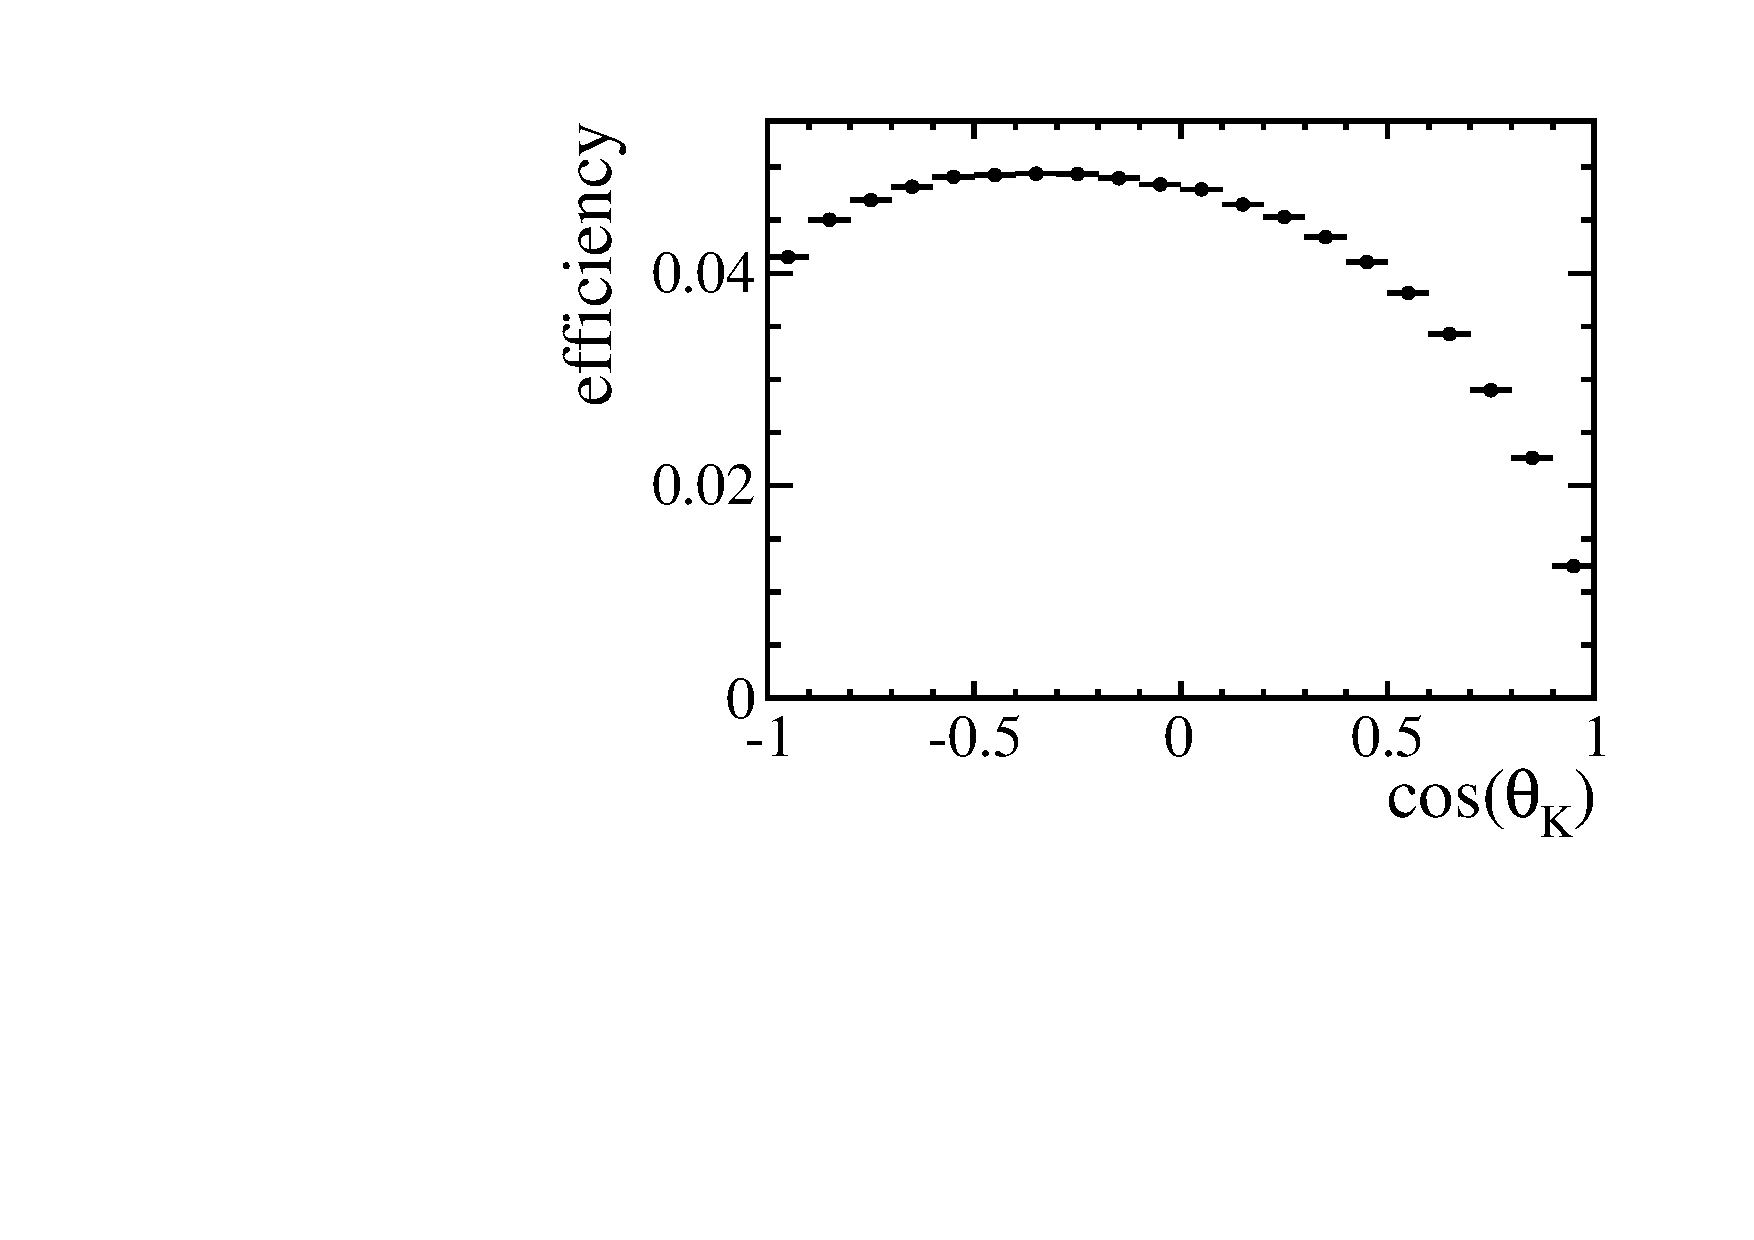
\includegraphics[width=0.48\columnwidth]{chapter5/figs/phsp_ctk_eff_dist.pdf}}
\subfigure[]{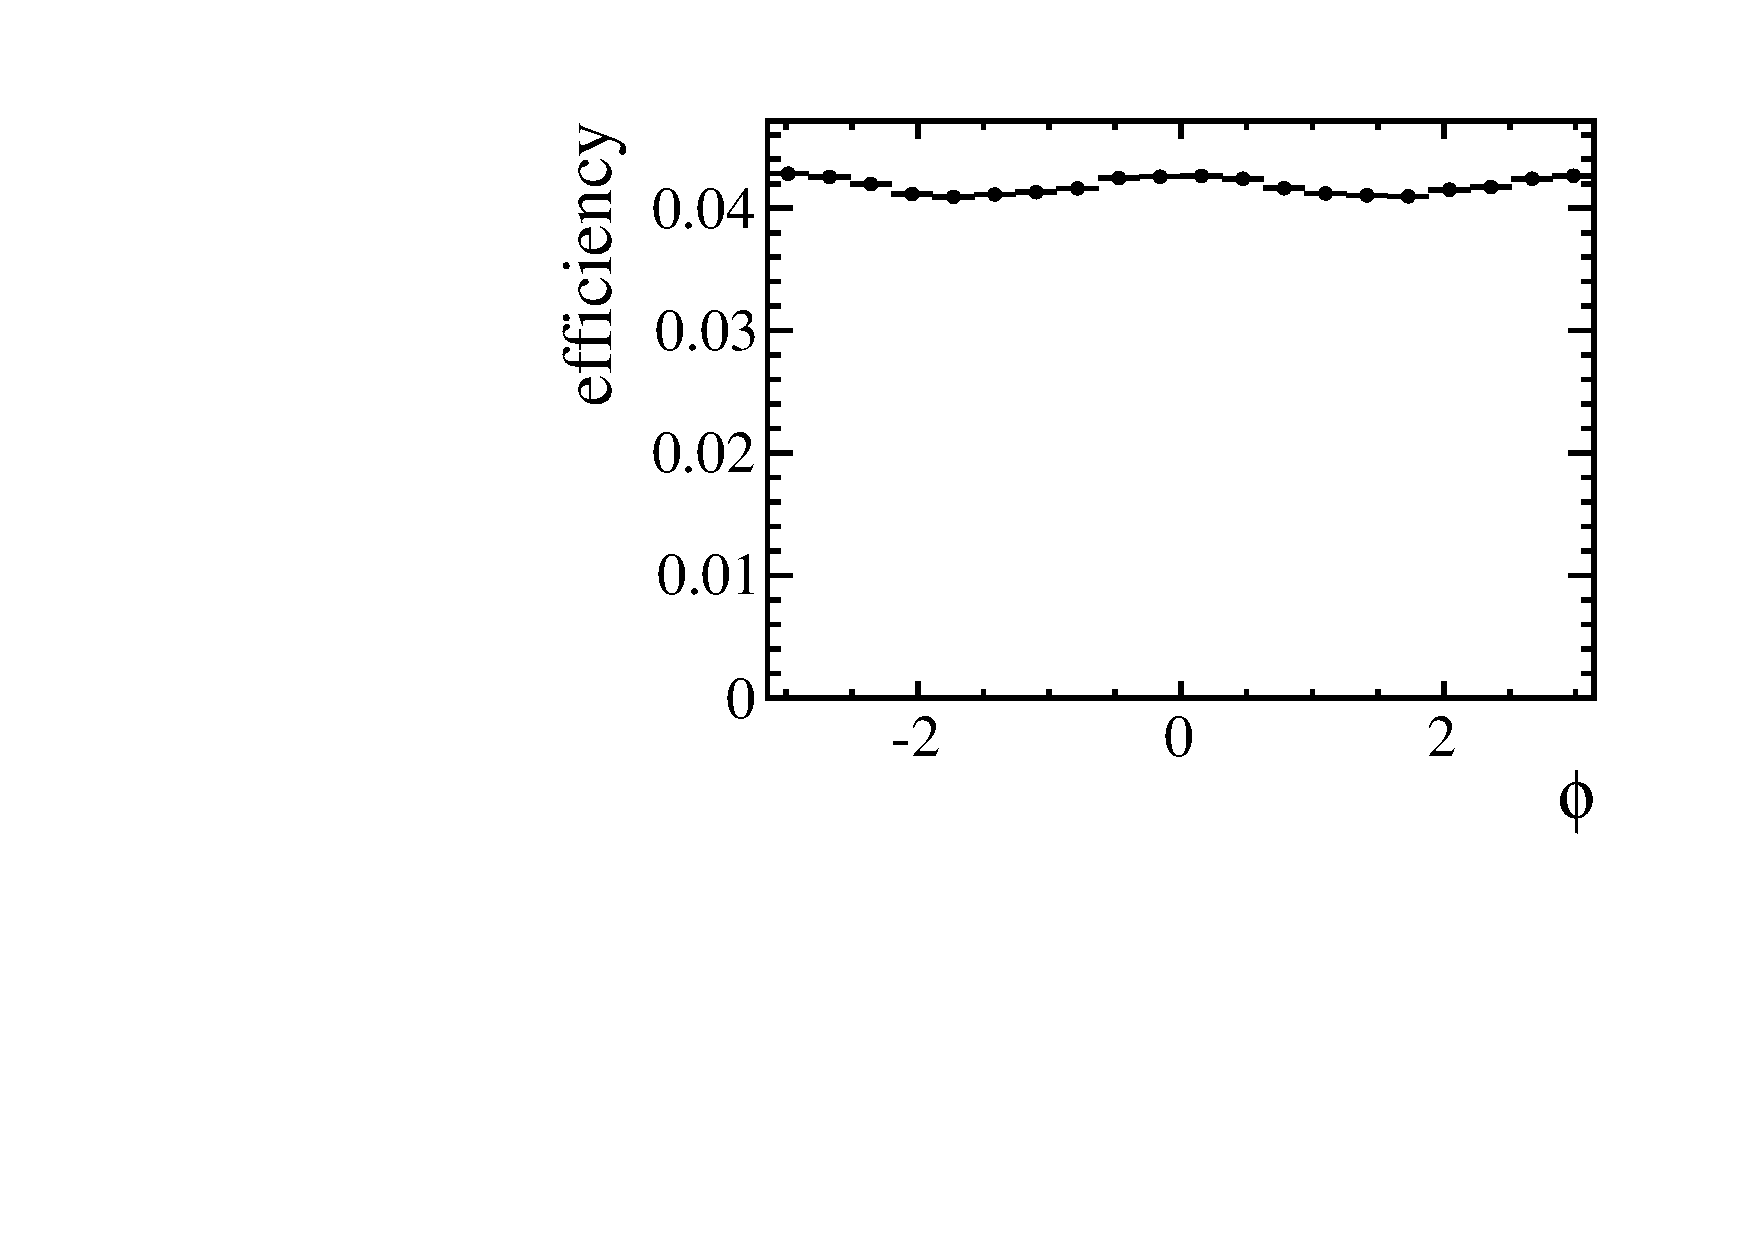
\includegraphics[width=0.48\columnwidth]{chapter5/figs/phsp_phi_eff_dist.pdf}}
\caption[The selection efficiency for \BdToKstmm on simulation]
{The efficiency for selected phase space simulated \BdToKstmm candidates as a function of (a) \qsq, (b) \ctl, (c) \ctk and (d) $\phi$. 
There is a reasonably symmetric acceptance in \ctl and an asymmetric acceptance effect in \ctk. 
The acceptance in \qsq varies across the full range and there is a very small acceptance effect in $\phi$.
 ~\label{fig:phspeff}}
\end{figure}
Is is possible to see the symmetric acceptance at high \ctl, due to 'backward-going' muons in the rest frame of the \Bd that have a very low momenta in the lab frame.
There is an asymmetric acceptance for \ctk from the same effect but the asymmetry is due to the difference in masses of the \kaon and the \pion. 
The different momentum spectra for the kaon and the pion is also affected by both the tracking efficiency and by the particle identification efficiency.
This is where most of the data/simulation corrections have a significant effect.

The total acceptance effect for a four-body decay is a function of the kinematic angles and invariant masses of the di-muon pair and the \kpi pair. 
The \psq window is assumed to be sufficiently small that there is no varying acceptance effect within it.
The angular analysis is performed in bins of \qsq requiring that the acceptance effect is corrected for on a finer level than the \qsq binning.


\subsection{A full 3D acceptance correction algorithm}
\label{sec:kstmm:ac:knnac}

One method of evaluating the efficiency as a function of phase space  is to count events before and after the selection
in fine bins of phase space.
This method was used in the first angular analysis of 0.38\invfb of data.
For an event at a particular point, the efficiency can be calculated by comparing the number of offline selected 
events with the number of generator level events `close' to that point : 
\begin{align}
\epsilon (\ctl, \ctk, q^2)_{r<R} = \frac{\offsel~(\delta d < R)  }{\genlvl~(\delta d < R)  } = \frac{n}{m}
\label{eq:eff}	
\end{align}
where $n$ is the number of weighted offline selected simulated events and $m$ is the number of generator level simulated events.
The distance $d$ is defined over the metric of the phase space and $R$ is the maximum distance within which events are chosen to contribute 
to the efficiency calculation.
The condition $\delta d < R$ defines a hyper-spheroid over the phase space.
The distance between event $i$ and event $j$, $\delta d_{ij}$, is given by
\begin{align}
\delta d_{ij} = \frac{1}{N_{\ctl}}( \ctl_i - \ctl_j  )^2 + \frac{1}{N_{\ctk}}( \ctk_i - \ctk_j) ^2 + \frac{1}{N_{\qsq}}( \qsq_i - \qsq_j) ^2 
\label{eq:distance}
\end{align}
where the normalisation factors, $(N_{\ctl}, N_{\ctk},N_{\qsq})$, are chosen such that the dimensions are each scaled between $[0,1]$. 
In order to collect events efficiently, a $k$-nearest neighbour algorithm was used to collect events in a small region of phase space. 

The error on the efficiency for a given bin is defined by the combination of the Poisson errors from $n$ and $m$, i.e.
\begin{align}
\sigma_{\epsilon} = \epsilon \times \sqrt{\frac{\sigma_n^2}{n^2} + \frac{1}{m}},
\end{align}
since the offline selection simulation is not a subset of the generation simulation.
The maximum radius $R$ is chosen such that the statistical error from the number of events within the hyper-spheroid is sufficiently small when compared to the size of the phase space. 
The average error and the average fractional error as a function of the radius of the hyper-spheroid is shown in Fig.~\ref{fig:errorvsradii}.
\begin{figure}[tbp]
\centering
\subfigure[]{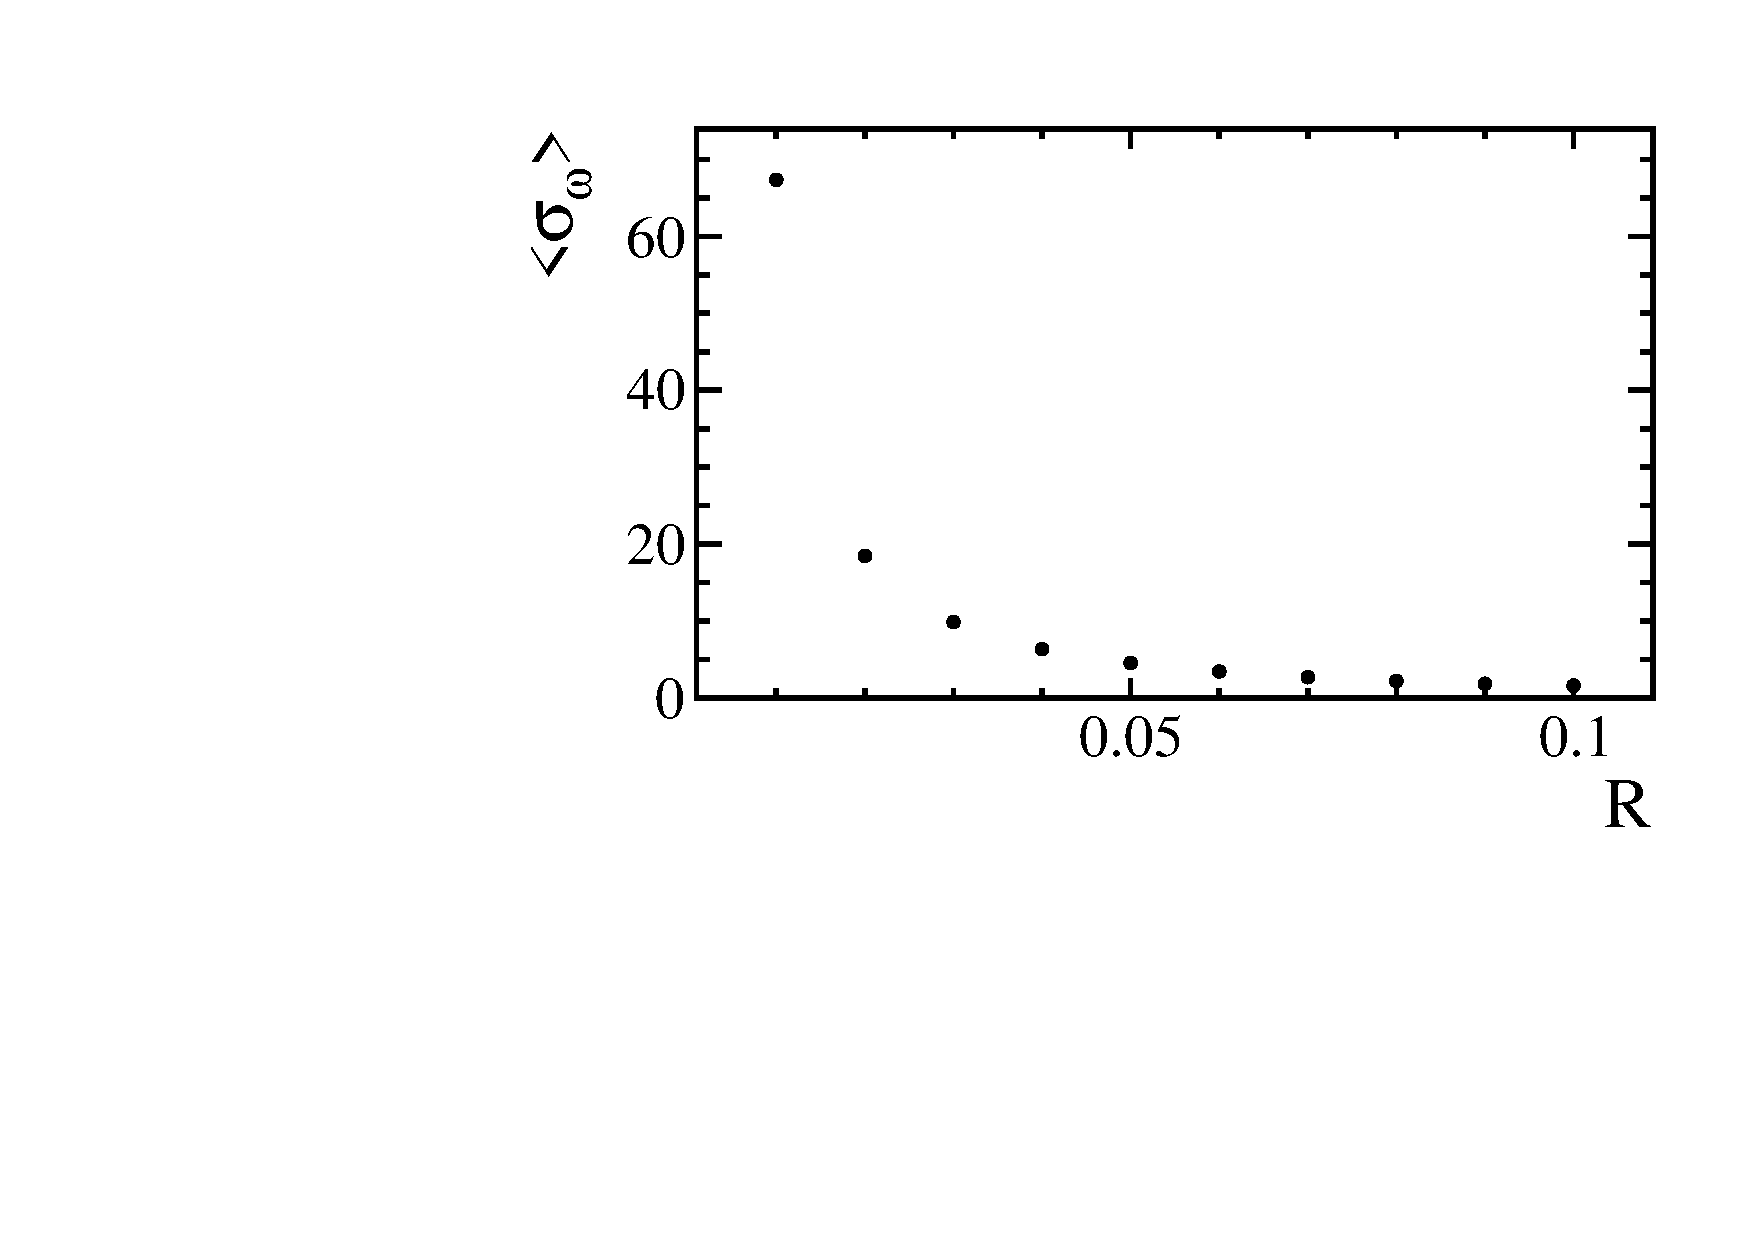
\includegraphics[width=0.48\columnwidth]{chapter5/figs/ac1/error_vs_radius.pdf}}
\subfigure[]{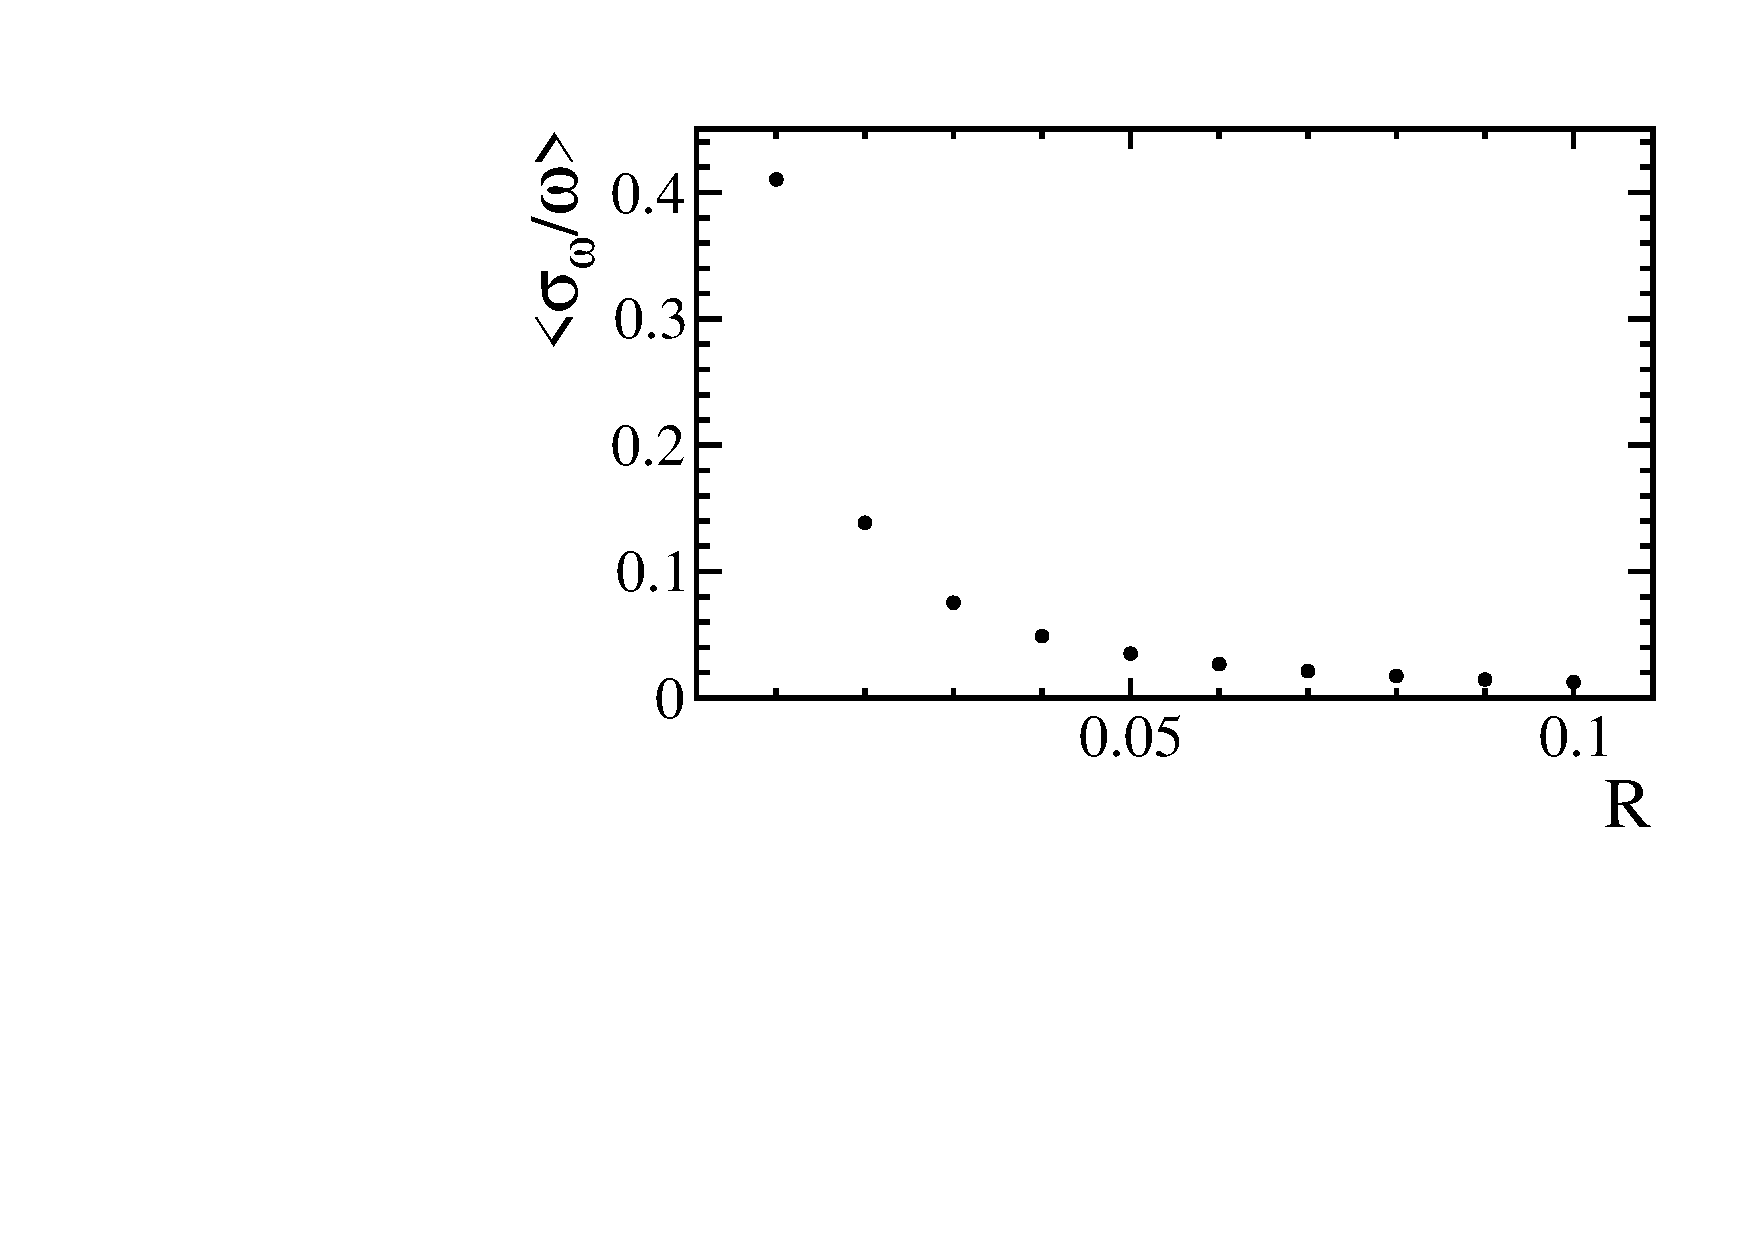
\includegraphics[width=0.48\columnwidth]{chapter5/figs/ac1/prop_error_vs_radius.pdf}}
\caption[The error on the acceptance correction weights.]
{ The average error (a) and the fractional error (b) on 150 weights for \BdToKstmm phase space simulated events for radii between 0.01 and 0.1. 
It is possible to see the $\sqrt{n^3}$ behaviour in the reduction of the error as more events are used to calculate the efficiency.
 ~\label{fig:errorvsradii} }
\end{figure}
The average error follows the expected Poisson behaviour but the fractional error is significant for radii of less than 0.02.

For the first angular analysis of 0.38\invfb of data, a radius of $R = 0.02$ was used to calculate an acceptance correction weight on an event-by-event basis.
This is chosen as a balance between contributing a large systematic error and retaining the accuracy on the correction.
The distribution of acceptance correction weights on data and the 
correlation between these weights and the angles are shown in Fig.~\ref{fig:ac1weights}.
\begin{figure}[tbp]
\centering
\subfigure[]{\includegraphics[width=0.48\columnwidth]{chapter5/figs/ac1/phasespace_weight_value.pdf}}
\subfigure[]{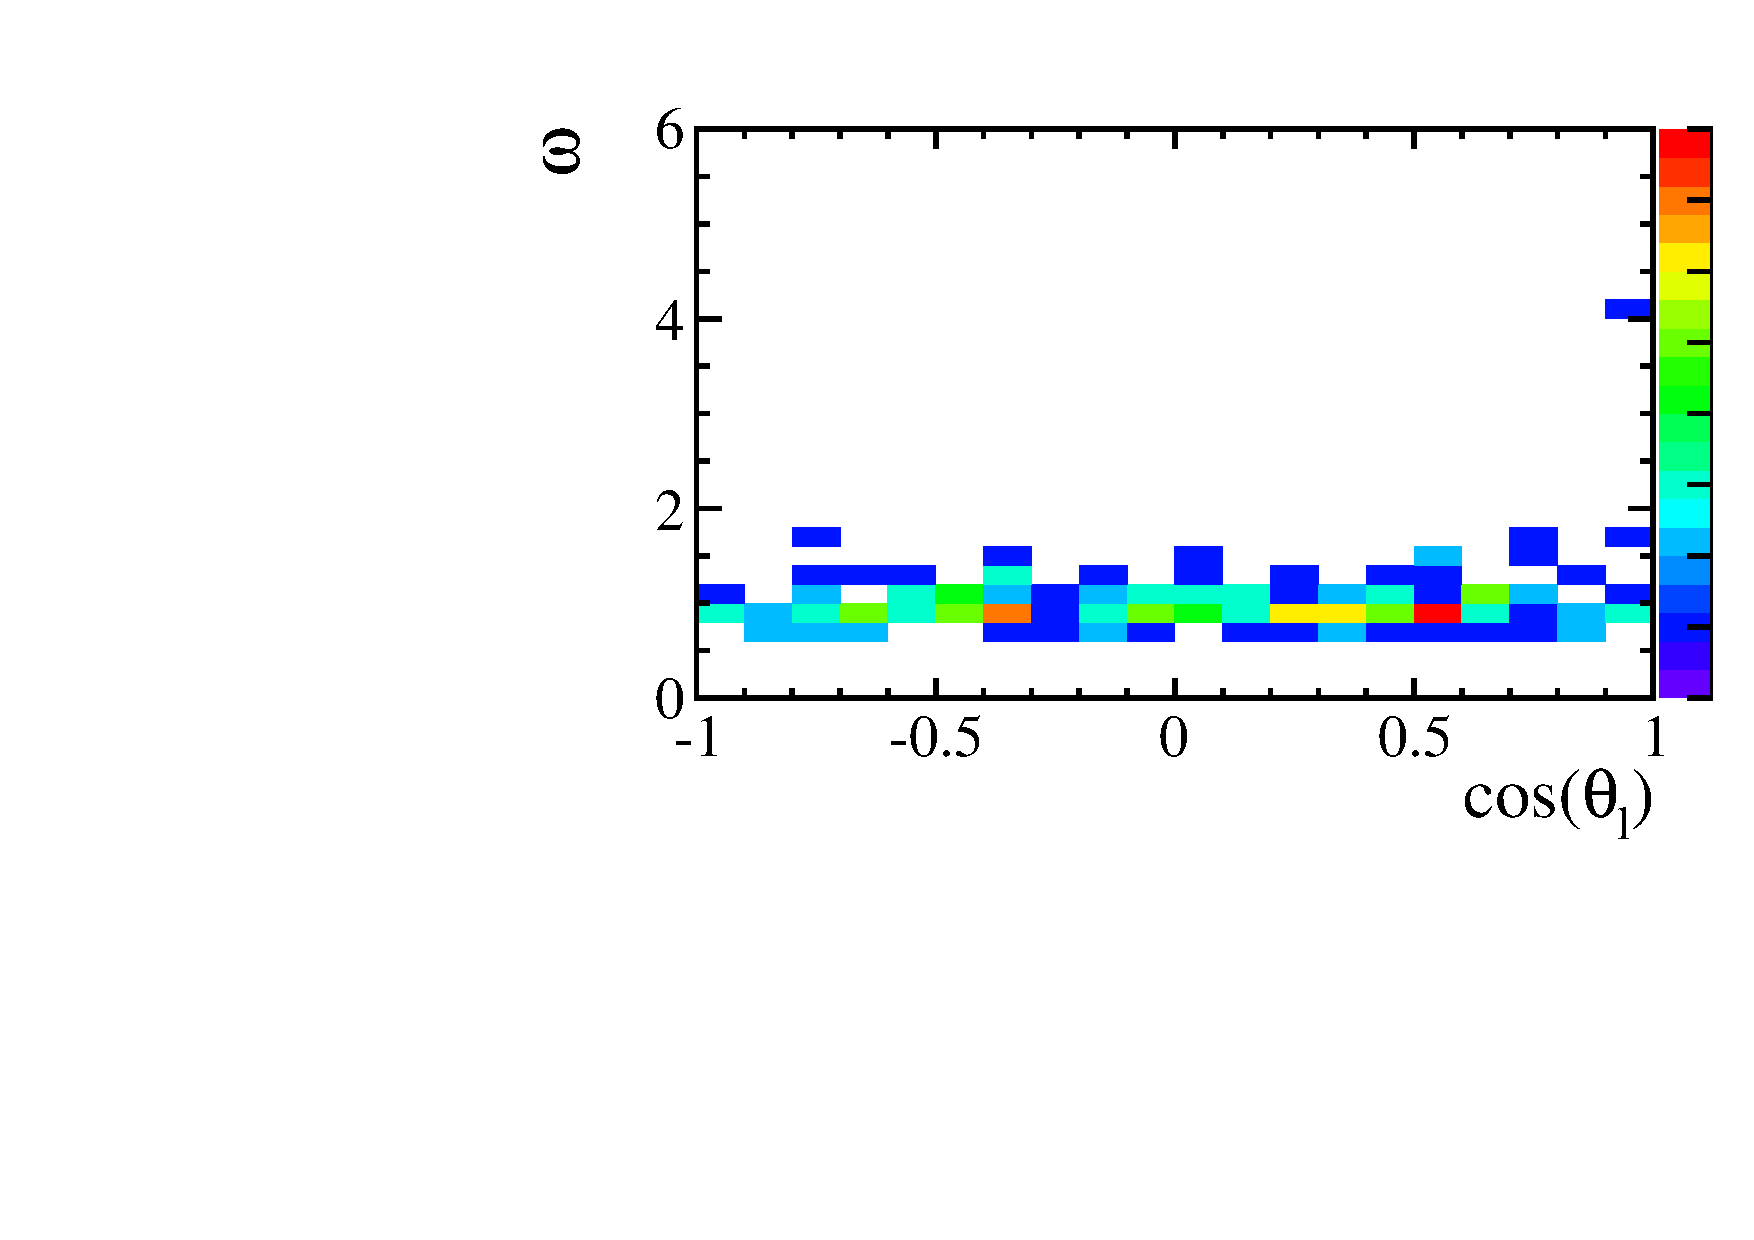
\includegraphics[width=0.48\columnwidth]{chapter5/figs/ac1/phasespace_weight_ctl.pdf}}
\subfigure[]{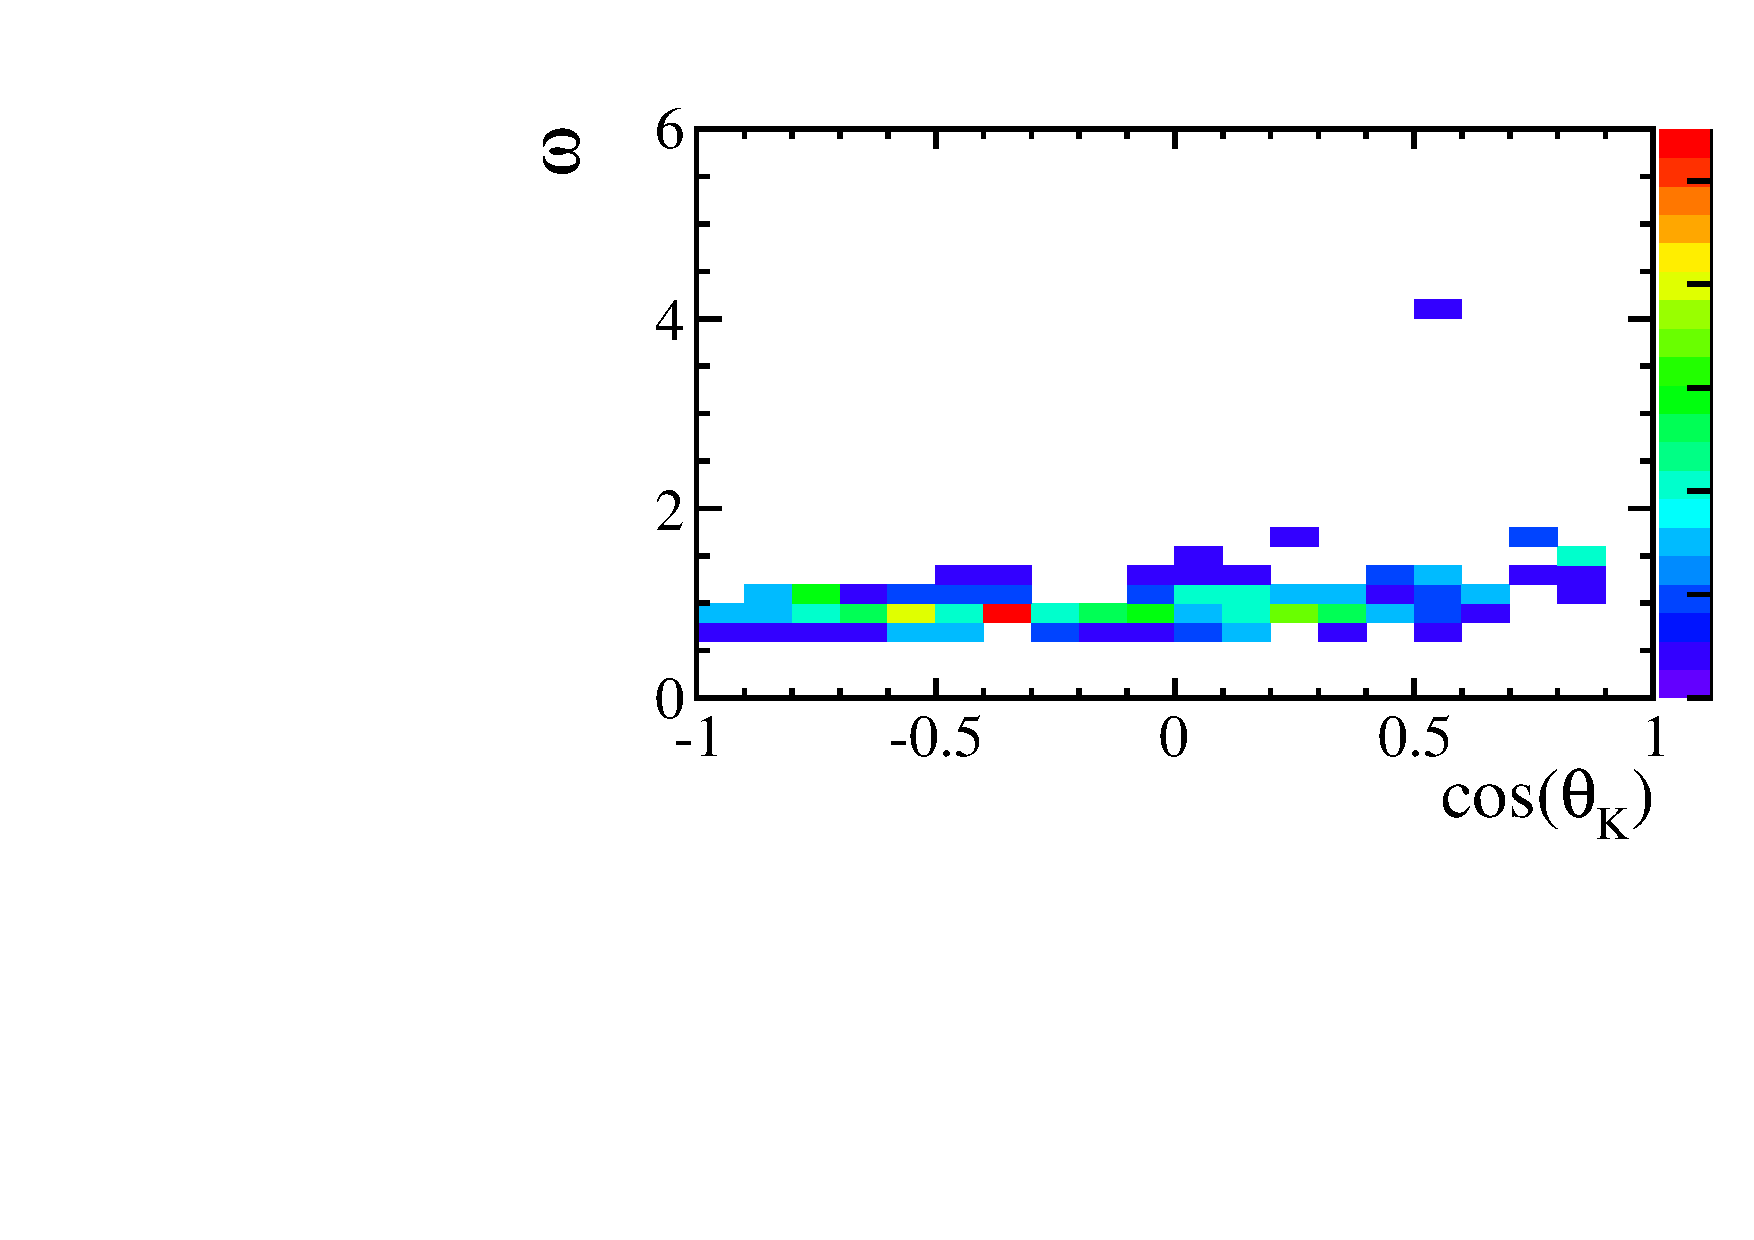
\includegraphics[width=0.48\columnwidth]{chapter5/figs/ac1/phasespace_weight_ctk.pdf}}
\caption[The weight distribution of acceptance corrected \BdToKstmm data.]
{ The distribution of weights for 150 phase space simulated \BdToKstmm events (a) and the correlation between 
the weights and \ctl (b) and \ctk (c). The weights are normalised such that the sum of weights is equal to the 
number of events. The high weights for extreme \ctk and \ctl can be seen. ~\label{fig:ac1weights} }
\end{figure}
It is possible to see that the weight values at extreme ($|\ctk|>0.8$) \ctk are higher than the weights in the centre.
The same effect can be seen in \ctl but to a lesser degree due to the integration over \qsq.
However, at low and high \qsq it is possible to see a variation of weights to accommodate the change in acceptance.

One limitation of the $k$-nearest-neighbour algorithm is 
that the error on the efficiency is entirely dominated 
by the number of offline selected simulated events at high \qsq.
If the data sample is binned more finely than the chosen collection radius $R$,
 then the `averaging effect' over the hyper-spheroid can be seen. 
In Fig.~\ref{fig:jpsikstardodgy}, an example of this can be seen in the large \BdToJpsiKstar sample.
\begin{figure}[tbp]
\centering
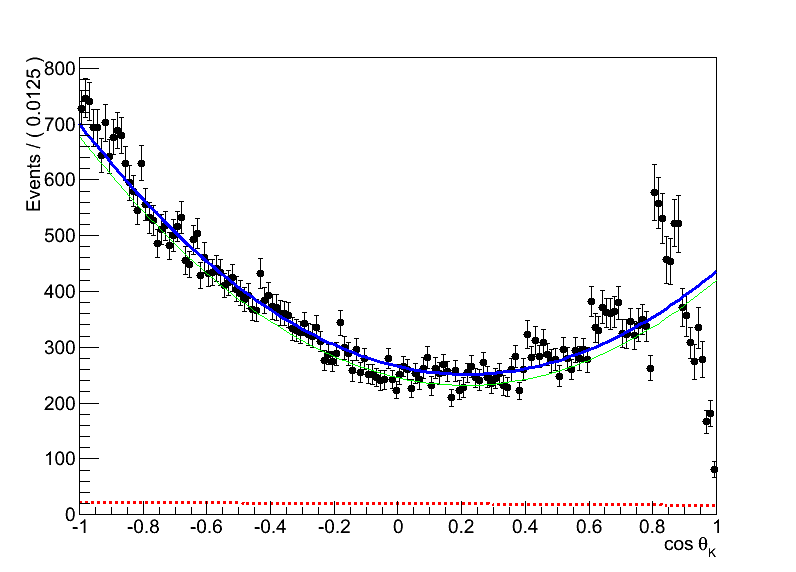
\includegraphics[width=0.48\columnwidth]{chapter5/figs/acceptance_variation_overbin.png}
\caption[ Weighted \BdToJpsiKstar events using a radius of $R = 0.05$. ]
{ Weighted \BdToJpsiKstar events using a radius of $R = 0.05$. 
The total expected number of events is shown in blue, along with the total expected number of signal events in green and the number of background events in red.
The effect of integrating over a rapidly varying efficiency is 
evident at high \ctk with a large statistics data sample. ~\label{fig:jpsikstardodgy} }
\end{figure}
A second limitation of the $k$-nearest-neighbour algorithm is the computational performance. 
The algorithm is at worst of order $\mathcal{O}(n)$ per event.
This can be simplified by only searching for neighbours in a small region of phase 
space, sufficient to encompass the subset of events within the radius $R$. 
As the number of events in the simulation has to scale with the size of the data, $n_{data}$,
 the overall scaling of the algorithm is $\mathcal{O}(n_{data}^2)$.
This, along with the required decrease in the systematic uncertainty on the efficiency calculation, 
necessitated the development of a more 
efficient acceptance algorithm for the angular analysis on the full 2011 dataset.

\subsection{A factorised acceptance correction algorithm}
\label{sec:kstmm:ac:facac}

In order to reduce the error on the acceptance correction beyond the reduction in statistical error for the full 2011 dataset, a factor of $1/\sqrt{3}$ was required to compensate for the threefold increase in data.
One solution to this issue, along with reducing the $\mathcal{O}(m^2)$ scaling of the $k$-nearest neighbour algorithm, 
is to model the distribution of events before and after selection using a \PDF.
The error on the fitted PDFs at a point in phase space is smaller than the error on a bin of $k$ events because 
the whole dataset is used to evaluate the efficiency.
%and PDFs, once fitted, can be evaluated at each point in phase space quickly.

In general, the efficiency function is not analytical so the choice of PDF to model the efficiency is entirely empirical.
The efficiency can be calculated at a particular point in phase space,
\begin{align}
\epsilon(\ctl, \ctk, \phi, \qsq) = \frac{n}{m} \times \frac{ S( \ctl, \ctk, \phi, \qsq ) }{ G( \ctl, \ctk, \phi, \qsq )  }  \, ,
\end{align}
where $S$ is the \PDF modelling the selected data and $G$ is the \PDF modelling the generator level data.
 The PDFs are normalised by the weighted number of events in the selected sample ($n$) divided by the number of generator level events ($m$).

Maximum use of the simulated events to give a large reduction in the error can be made by factorising the efficiency in the form,
\begin{align}
\epsilon(\ctl, \ctk, \phi,\qsq)  = \epsilon(\ctl)\times\epsilon(\ctk)\times\epsilon(\phi)\times\epsilon(\qsq) \, .
\end{align}
This factorisation is in general not possible due to the fact that there is a correlation between the angles and \qsq.
The efficiency for each of the angles for offline selected simulated phase space \BdToKstmm events 
 in a low \qsq bin are given in Fig.~\ref{fig:phspeff2d}. 
\begin{figure}[tbp]
\centering
\subfigure[\ctl v.s. \ctk]{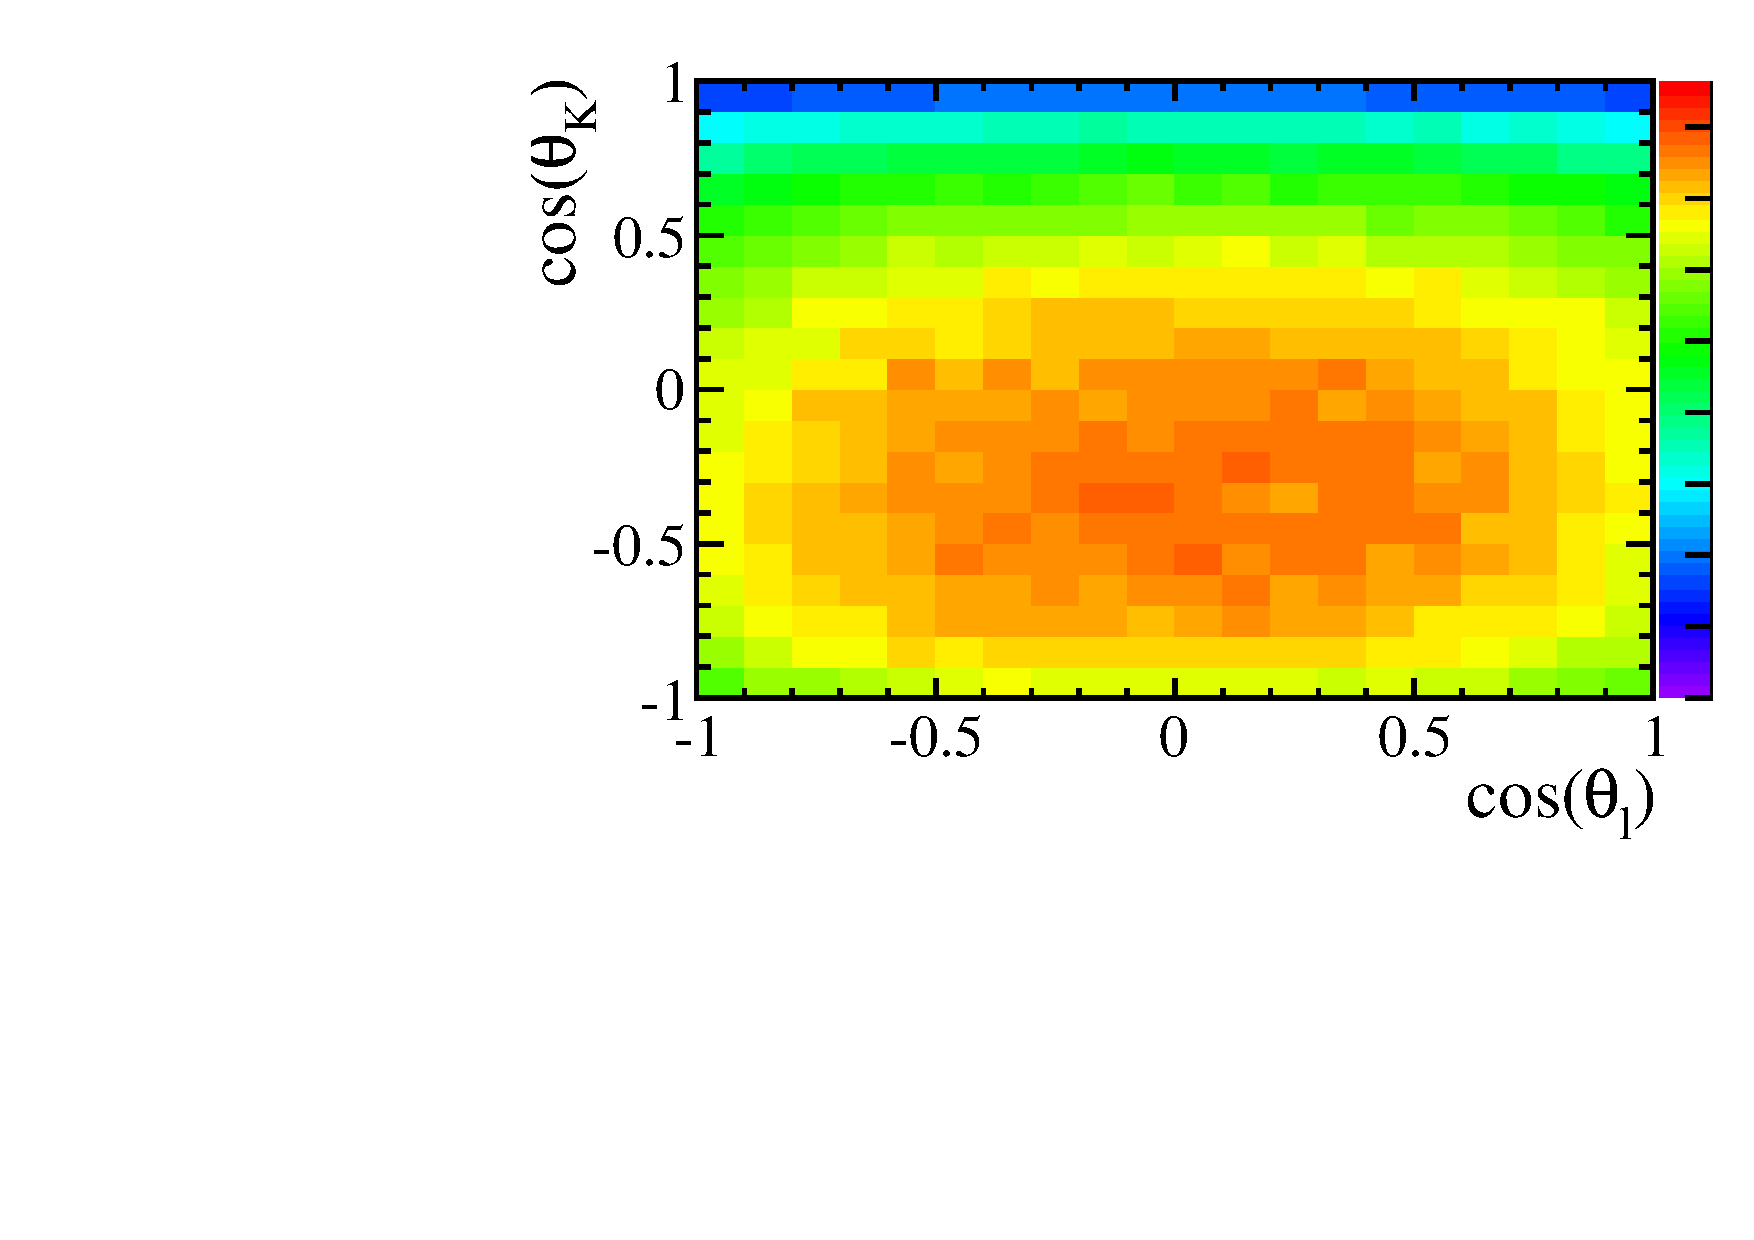
\includegraphics[width=0.48\columnwidth]{chapter5/figs/phsp_ctl_ctk_sel_dist.pdf}}
\subfigure[\ctl v.s. $\phi$]{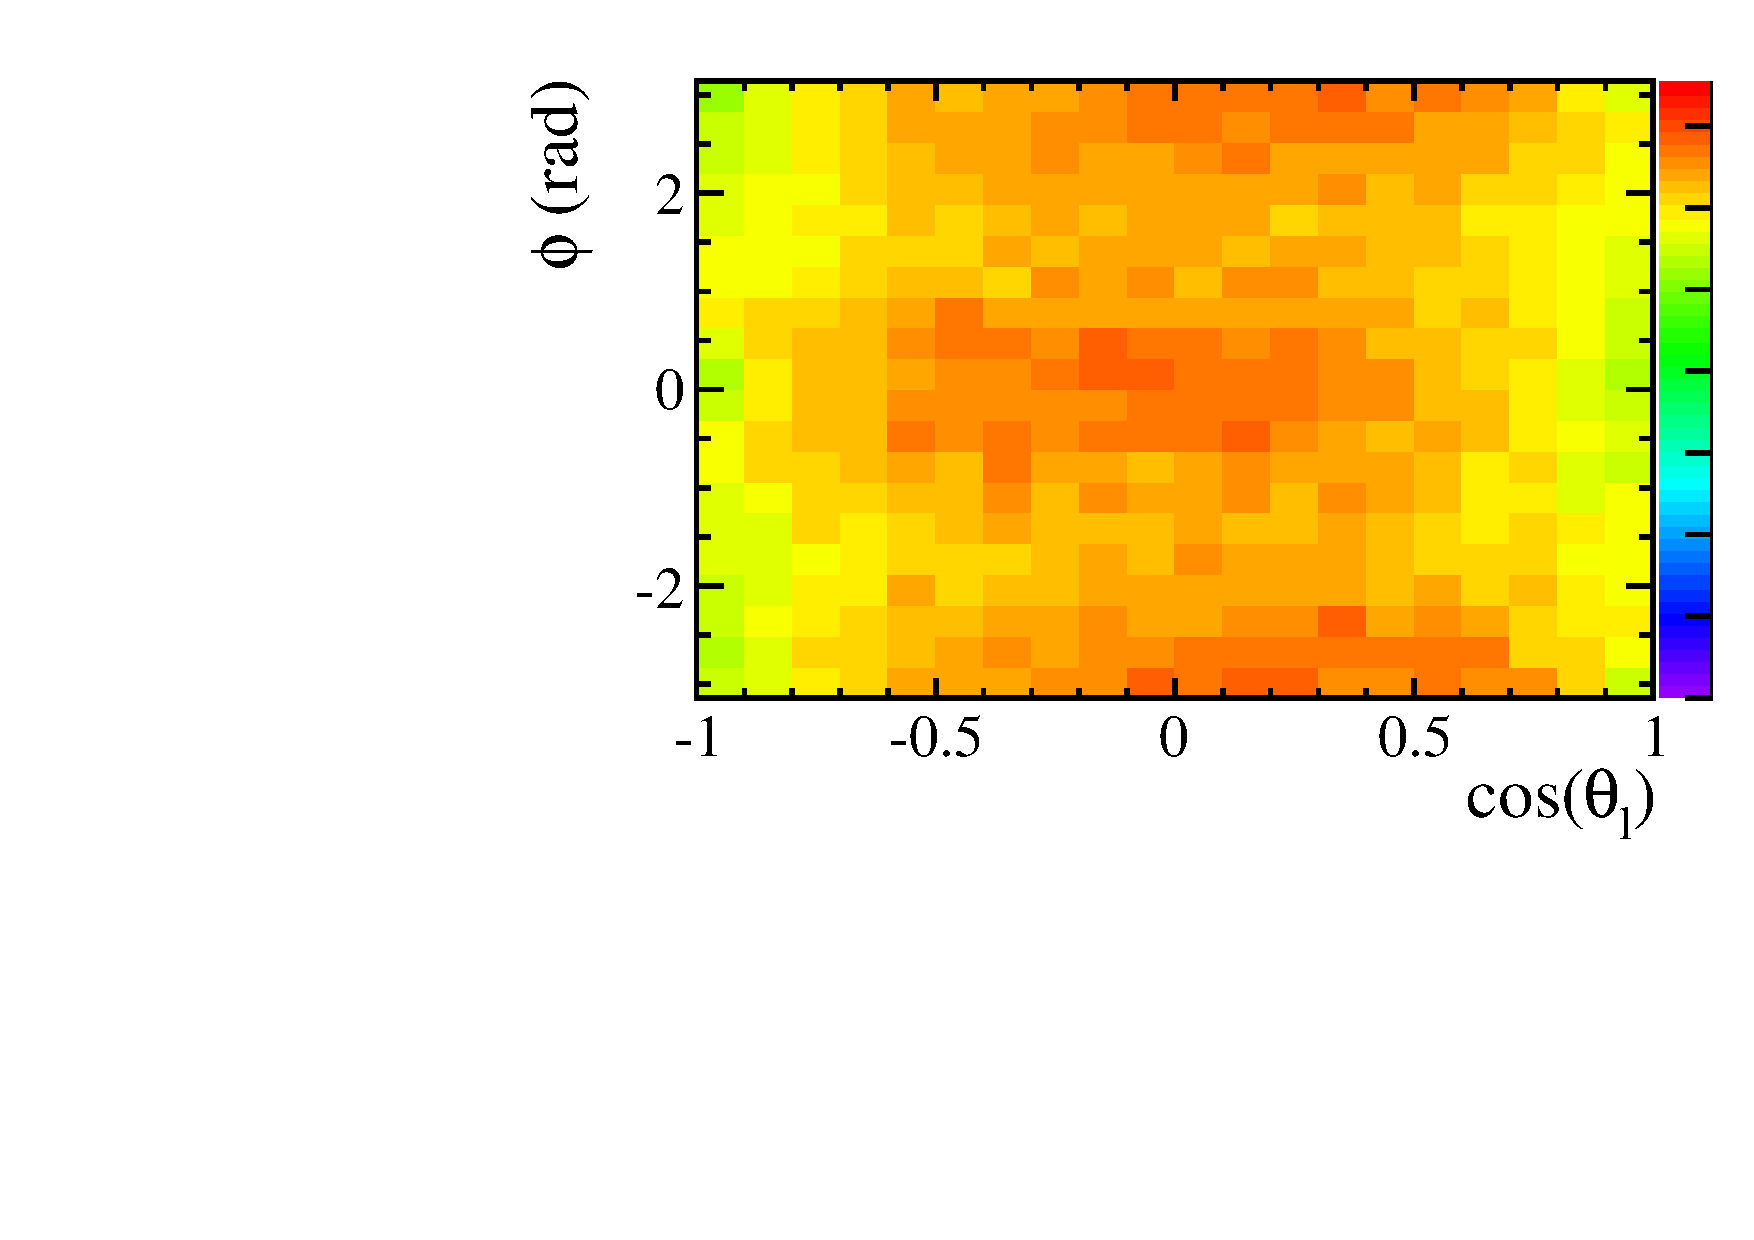
\includegraphics[width=0.48\columnwidth]{chapter5/figs/phsp_ctl_phi_sel_dist.pdf}}
\subfigure[\ctk v.s. $\phi$]{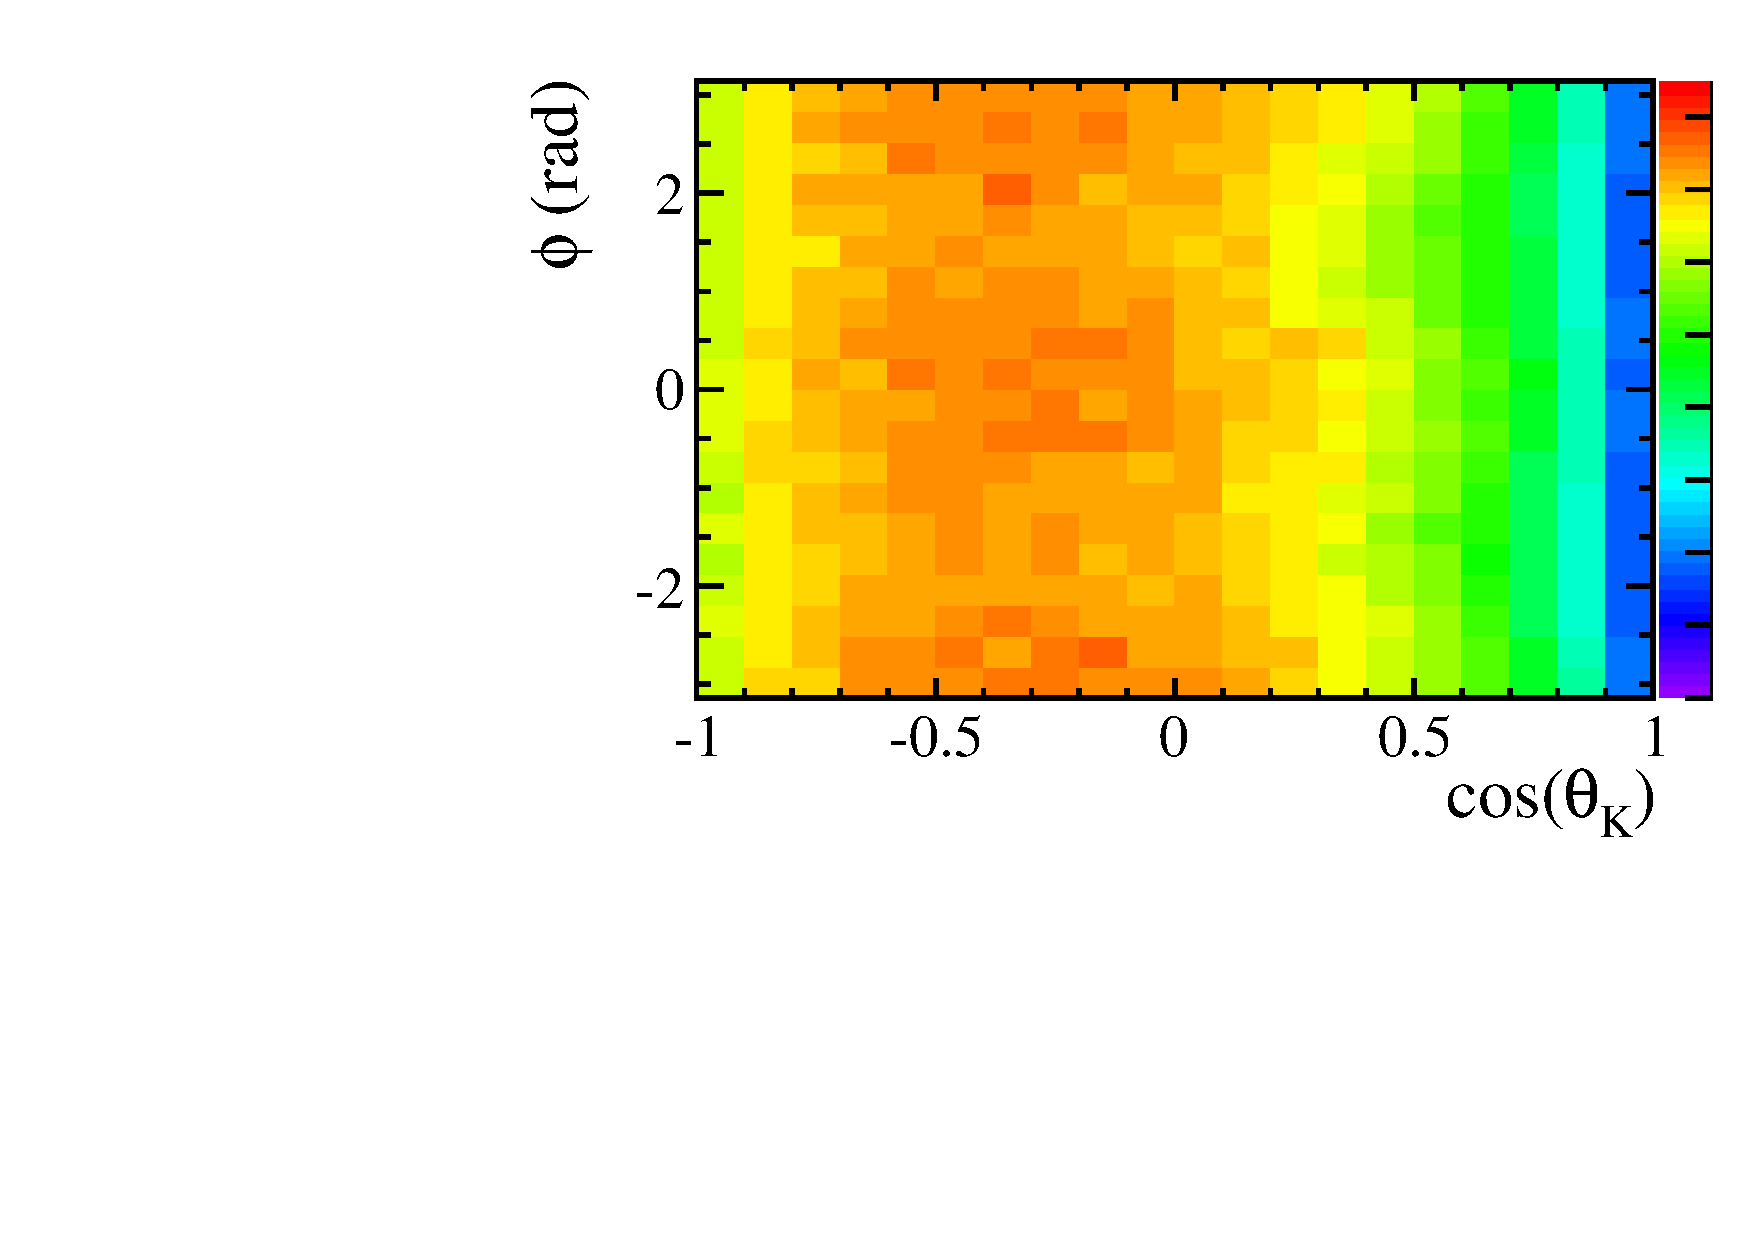
\includegraphics[width=0.48\columnwidth]{chapter5/figs/phsp_ctk_phi_sel_dist.pdf}}
\subfigure[\ctl v.s. \qsq]{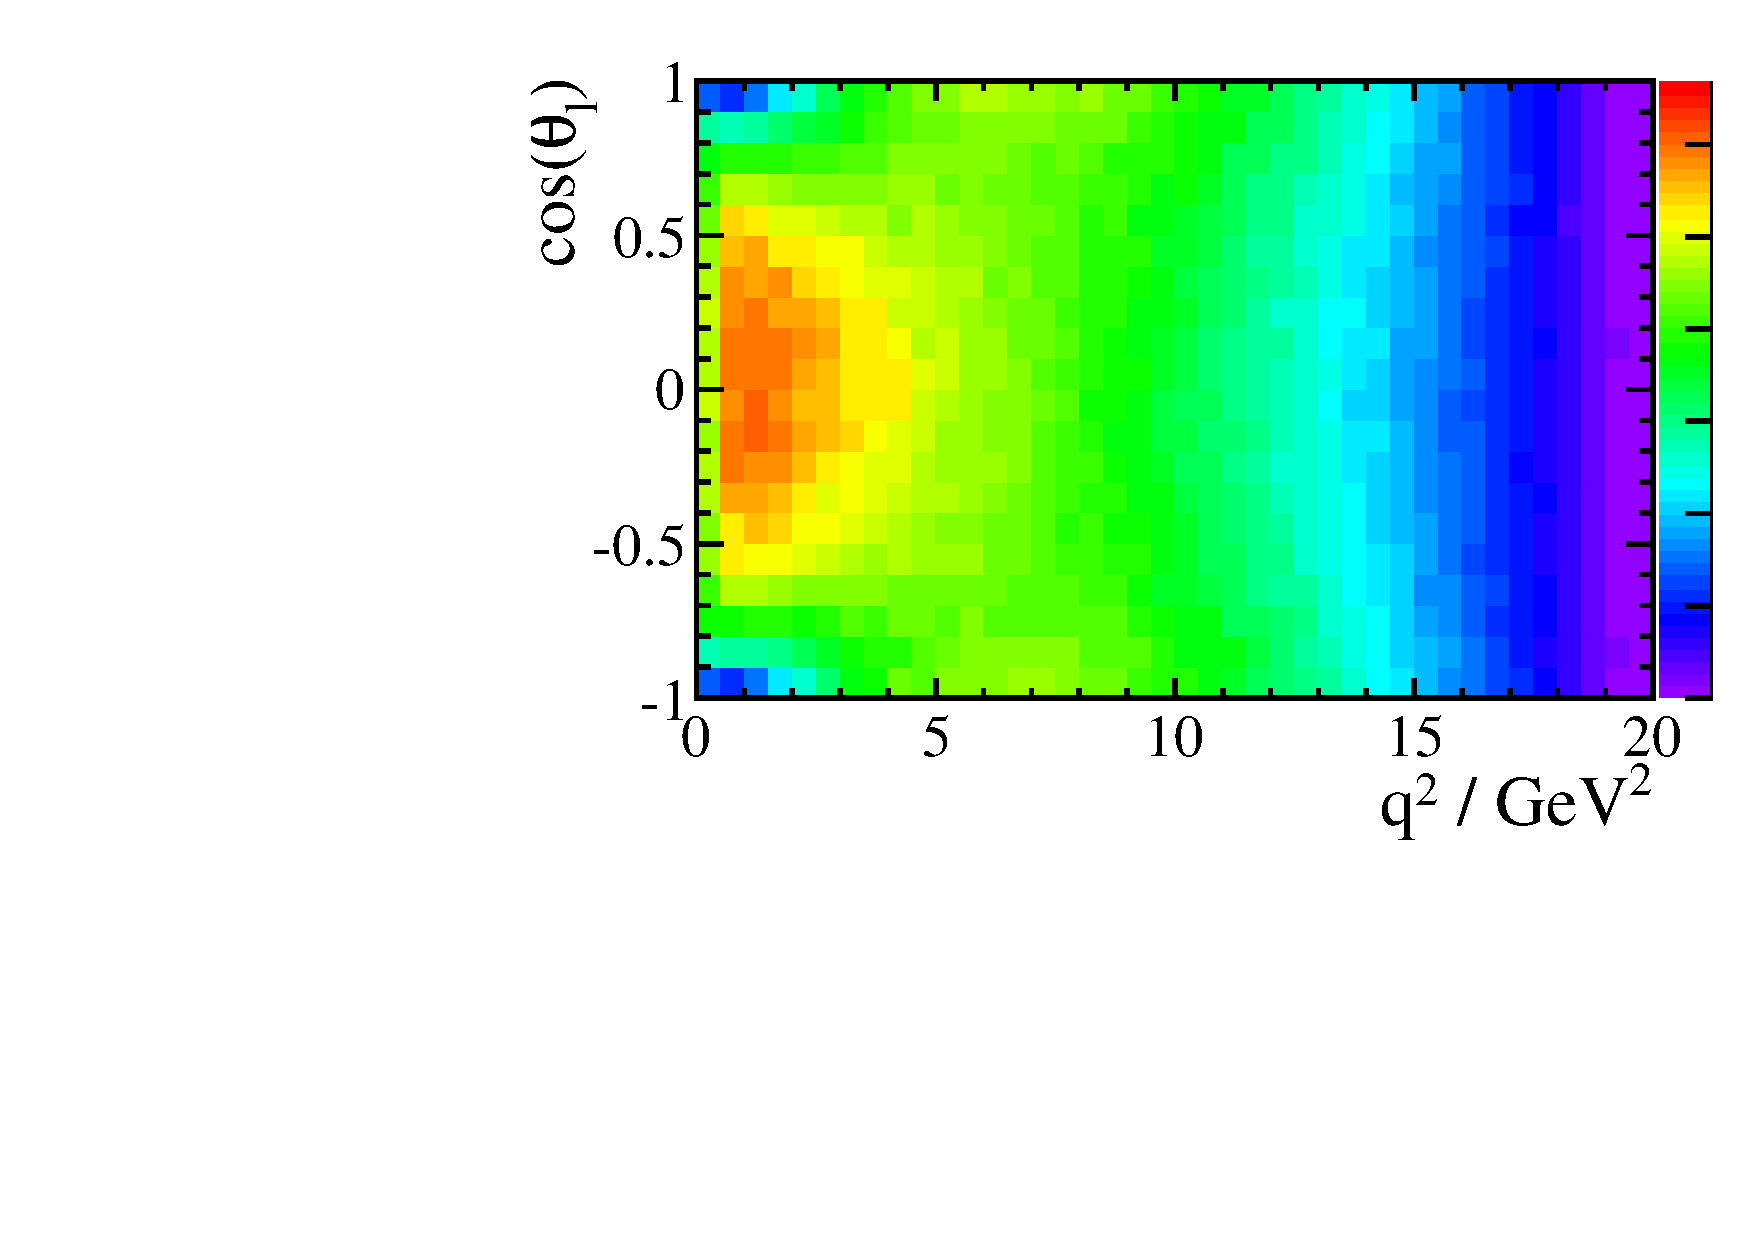
\includegraphics[width=0.48\columnwidth]{chapter5/figs/phsp_ctl_qsq_sel_dist.pdf}}
\subfigure[\ctk v.s. \qsq]{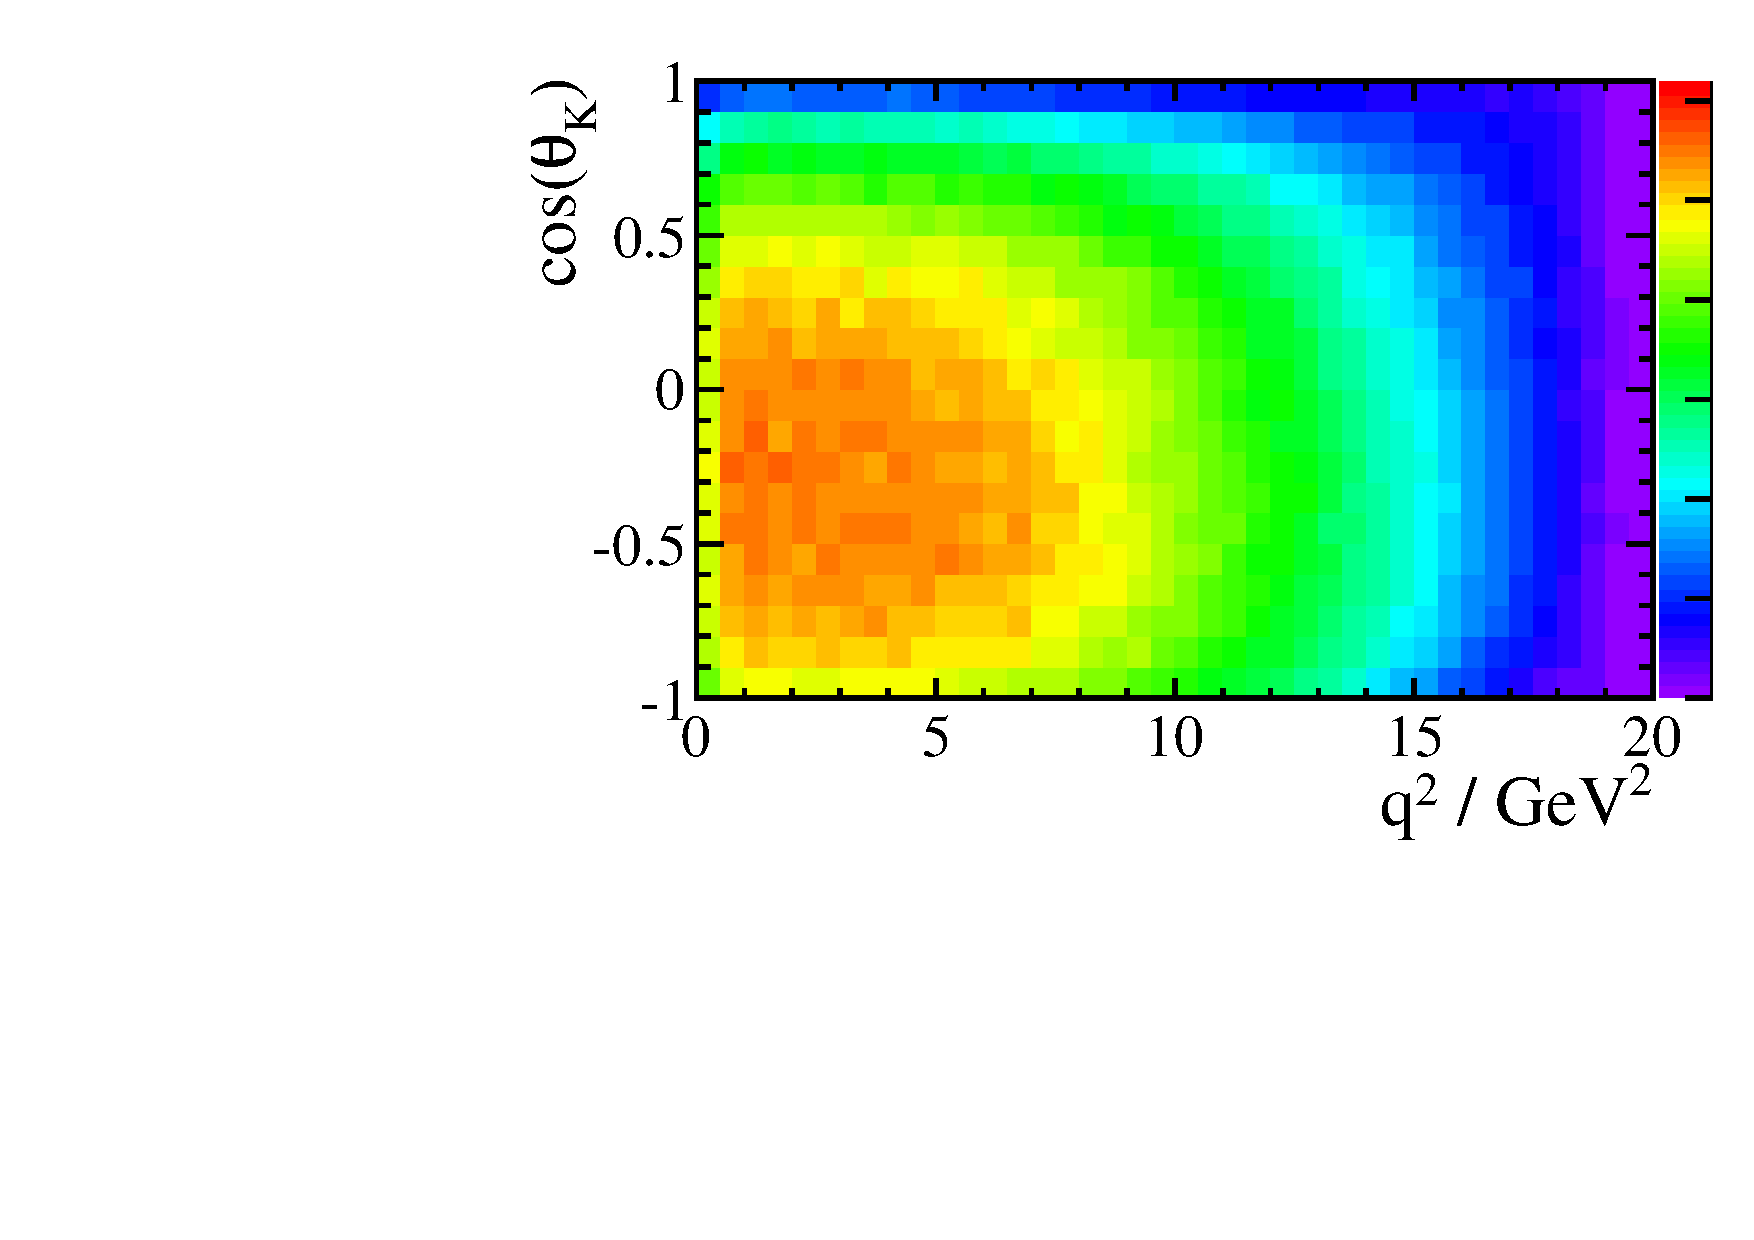
\includegraphics[width=0.48\columnwidth]{chapter5/figs/phsp_ctk_qsq_sel_dist.pdf}}
\subfigure[$\phi$ v.s. \qsq]{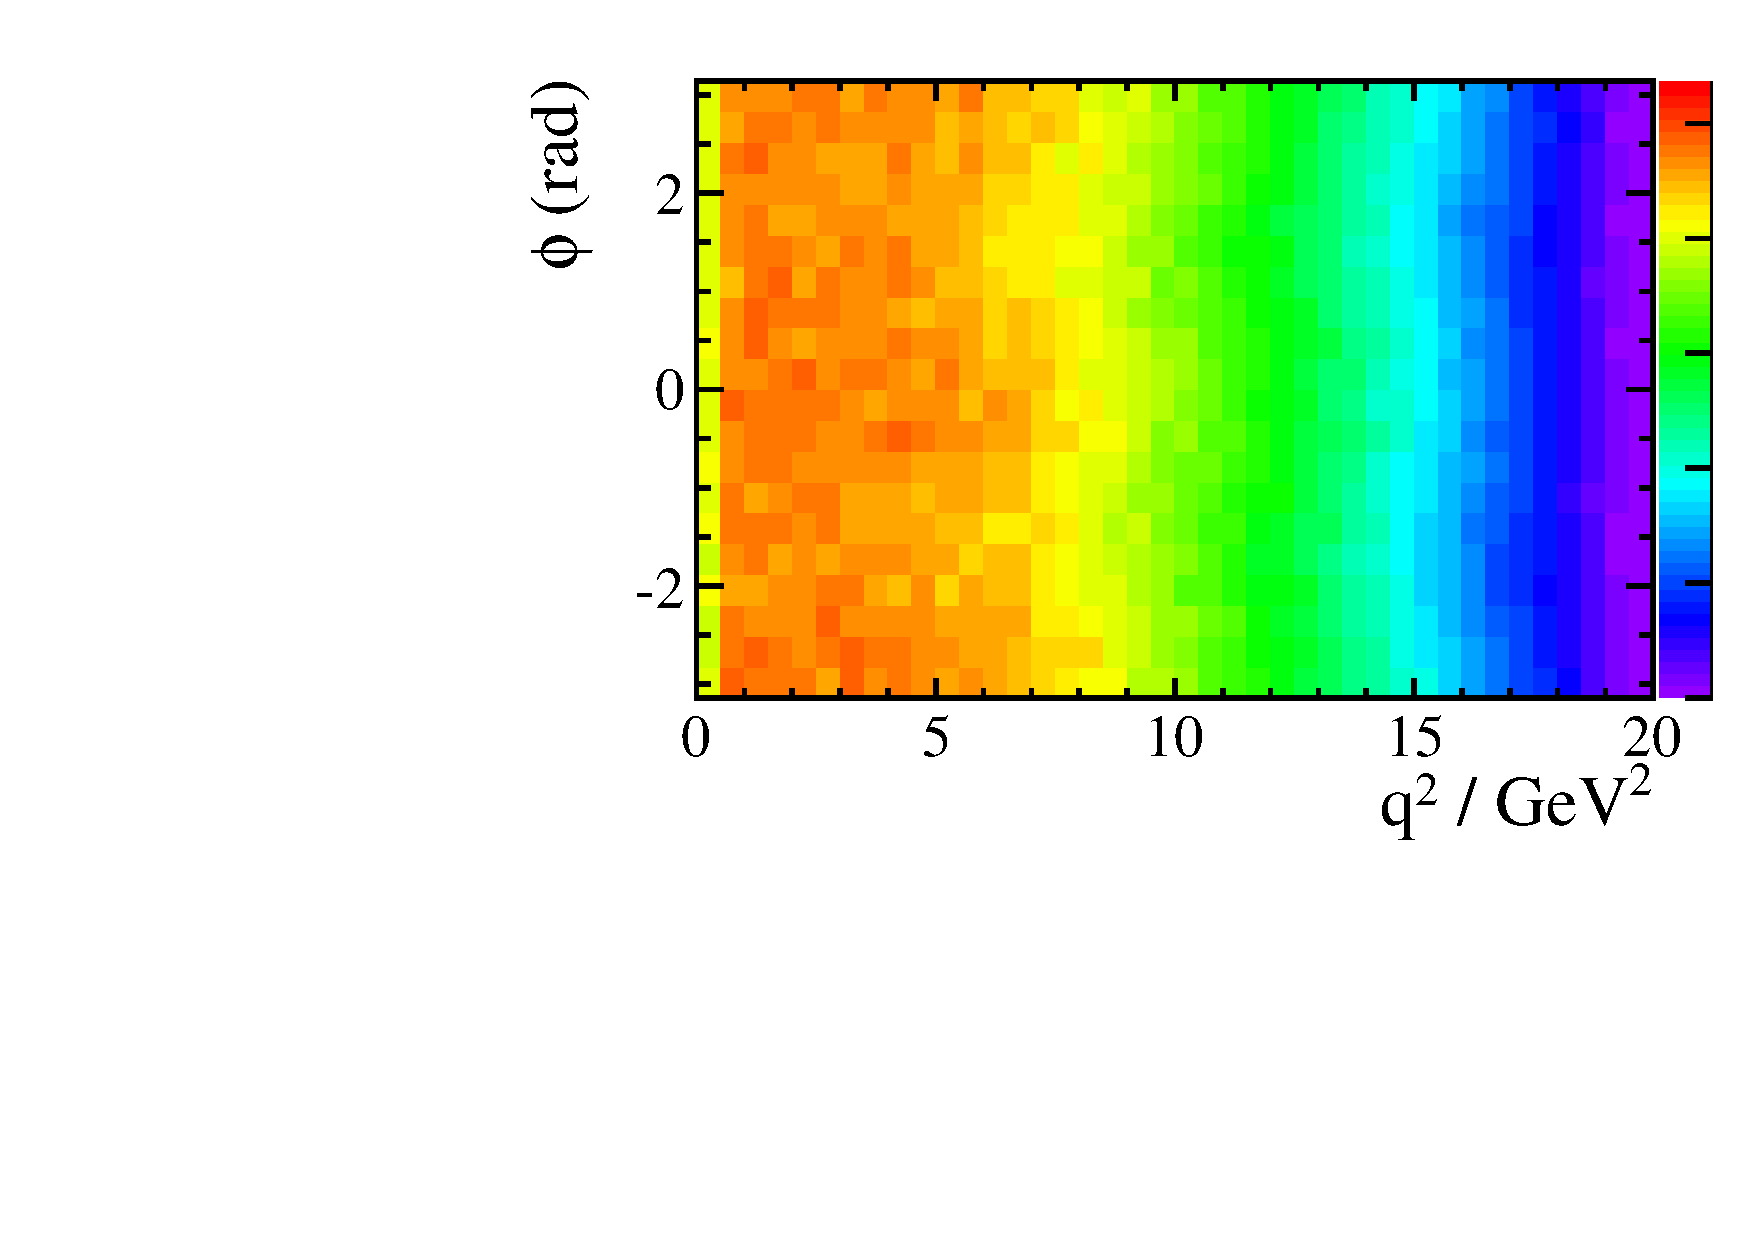
\includegraphics[width=0.48\columnwidth]{chapter5/figs/phsp_phi_qsq_sel_dist.pdf}}
\caption[Two dimensional efficiency for \BdToKstmm simulation.]
{The efficiency for selected phase space simulated \BdToKstmm events. 
In (a), (b), and (c), events are selected in the low \qsq bin ($1 < \qsq < 2 \gevgevcccc$). 
In (d), (e) and (f), the correlation between the individual angles and the full \qsq range is shown.
~\label{fig:phspeff2d} } 
\end{figure}
%It is possible to see the the efficiency is correlated with \qsq but 
%there is no significant correlation between the angles on the level of the binning shown here. 
From this it is possible to see that the efficiency function varies as \qsq, but there is no significant non-factorisable effect in the angles.
This means that the PDFs must be binned in \qsq but can be factorised between the angles.
The efficiency function for a bin in \qsq is given by 
\begin{align}
\epsilon(\ctl, \ctk, \phi, x<\qsq<y)  = \left( \frac{n_{(x<\qsq<y)} }{m_{(x<\qsq<y)} }\right) \times  S_L(\ctl) \times S_K( \ctk ) \times  S_P( \phi ) 
\end{align}
where $S_i$ is the \PDF describing the distribution of offline selected phase 
space events for each angle. 
The generator level \PDF ($G$) is uniform as a function of each of the angles and can be integrated out.

A non-uniform binning scheme was chosen to take advantage of the uneven distribution of the simulated statistics in \qsq. 
At low \qsq, where statistics are higher, bins of 0.1 \gevgevcccc are used. 
Bins of 0.2 \gevgevcccc are used in the \qsq range from 1 to 6 \gevgevcccc, and bins of 0.5 \gevgevcccc above 6 \gevgevcccc 
to the upper limit of 19\gevgevcccc .
These bins are chosen such that there are at least fifteen thousand offline 
selected events in the least populated bin from a total of two million simulated events.

The one-dimensional efficiency is modelled as a 6th order Chebychev polynomial~\cite{CHEBYCHEV}
and normalised such that the polynomial integrates to 1,
\begin{align}
\int S_i(\text{x};p_0,p_1,p_2,p_3,p_4,p_5)\ \deriv\text{x} = 1 \, ,
\end{align}
where $p_i$ are the coefficients of the polynomial. 
In order to acquire higher statistics in each \qsq bin, further reducing the error on the \PDF, 
the efficiency functions for \ctl and $\phi$ are assumed to be symmetric around 0. 
This symmetry holds to the level of CP-violating detector effects which are assumed to be less than 5\%.
The total efficiency is given by
\begin{align}
\epsilon(\qsq,\ctl,\ctk,\phi)_{(x<\qsq<y)} &= \left( \frac{n_{(x<\qsq<y)} }{m_{(x<\qsq<y)} }\right) \nonumber\\
& \times S_L(\ctl;0,a_1,0,a_3,0,a_5) \nonumber\\
& \times  S_K(\ctk;b_0,b_1,b_2,b_3,b_4,b_5) \nonumber\\
& \times S_P(\phi;0,c_1,0,c_3,0,c_5)
\end{align}
where the even (odd) parameters describe the symmetric (anti-symmetric) components of the polynomial.
The efficiency \PDFs for \ctl, \ctk and \varphi for an example low \qsq bin are shown in Fig.~\ref{fig:facpdfs}.
\begin{figure}[tbp]
\centering
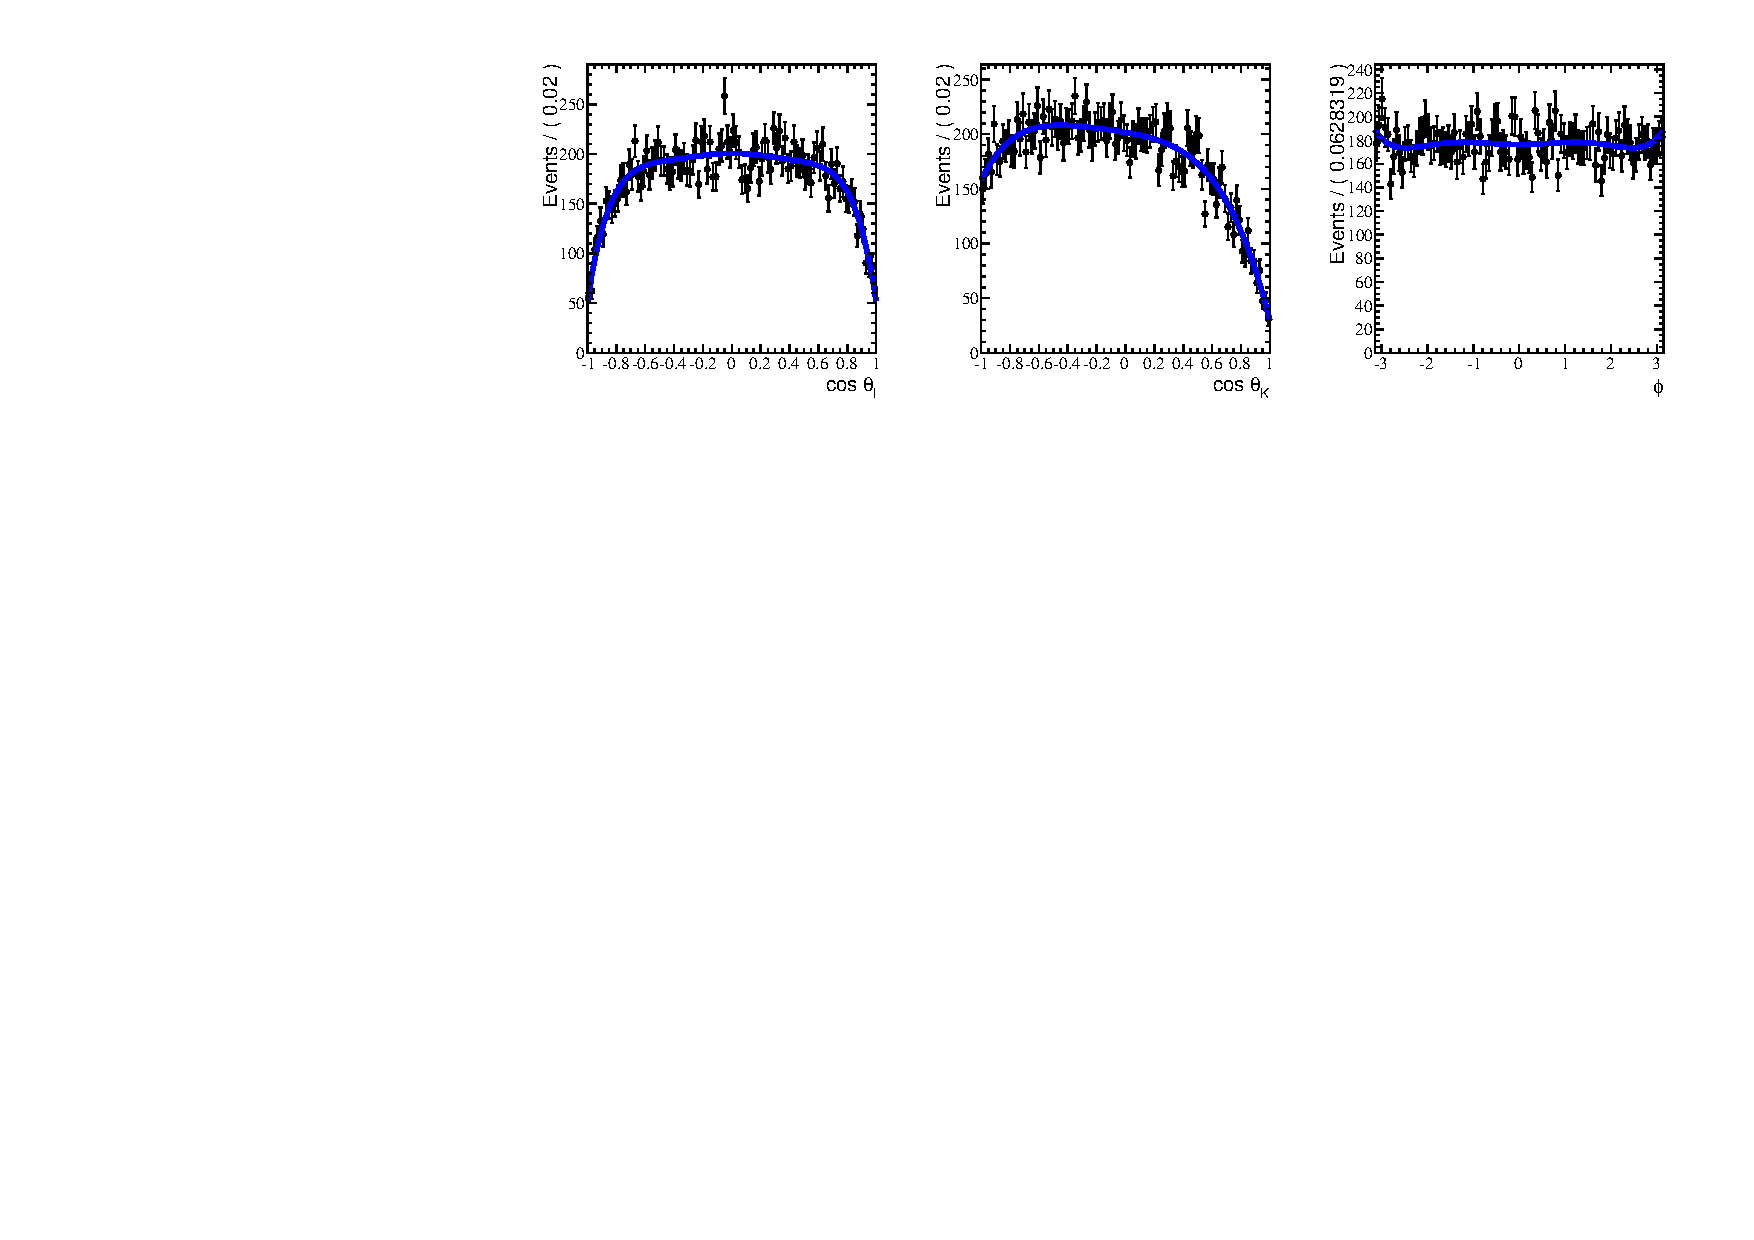
\includegraphics[width=0.96\columnwidth]{chapter5/figs/kstmm_fac_eff_pdfs_nqsqbins.pdf}
\caption[ The simulated \BdToKstmm events and the fitted PDF describing the selected events in \ctl (left), \ctk (middle)
and $\phi$ (right) for the \qsq bin from 0.1 to 0.2 \gevgevcccc.]
{ The angular efficiency in each of the angles for the \qsq bin from 0.1 to 0.2 \gevgevcccc.
The factorised \PDF was fitted to phase space \BdToKstmm simulation. ~\label{fig:facpdfs} }
\end{figure}

The distribution of weights on ten thousand phase space events is given in Fig~\ref{fig:ac2weights}.
\begin{figure}[tbp]
\centering
\subfigure[]{\includegraphics[width=0.48\columnwidth]{chapter5/figs/ac2/phasespace_weight_value.pdf}}
\subfigure[]{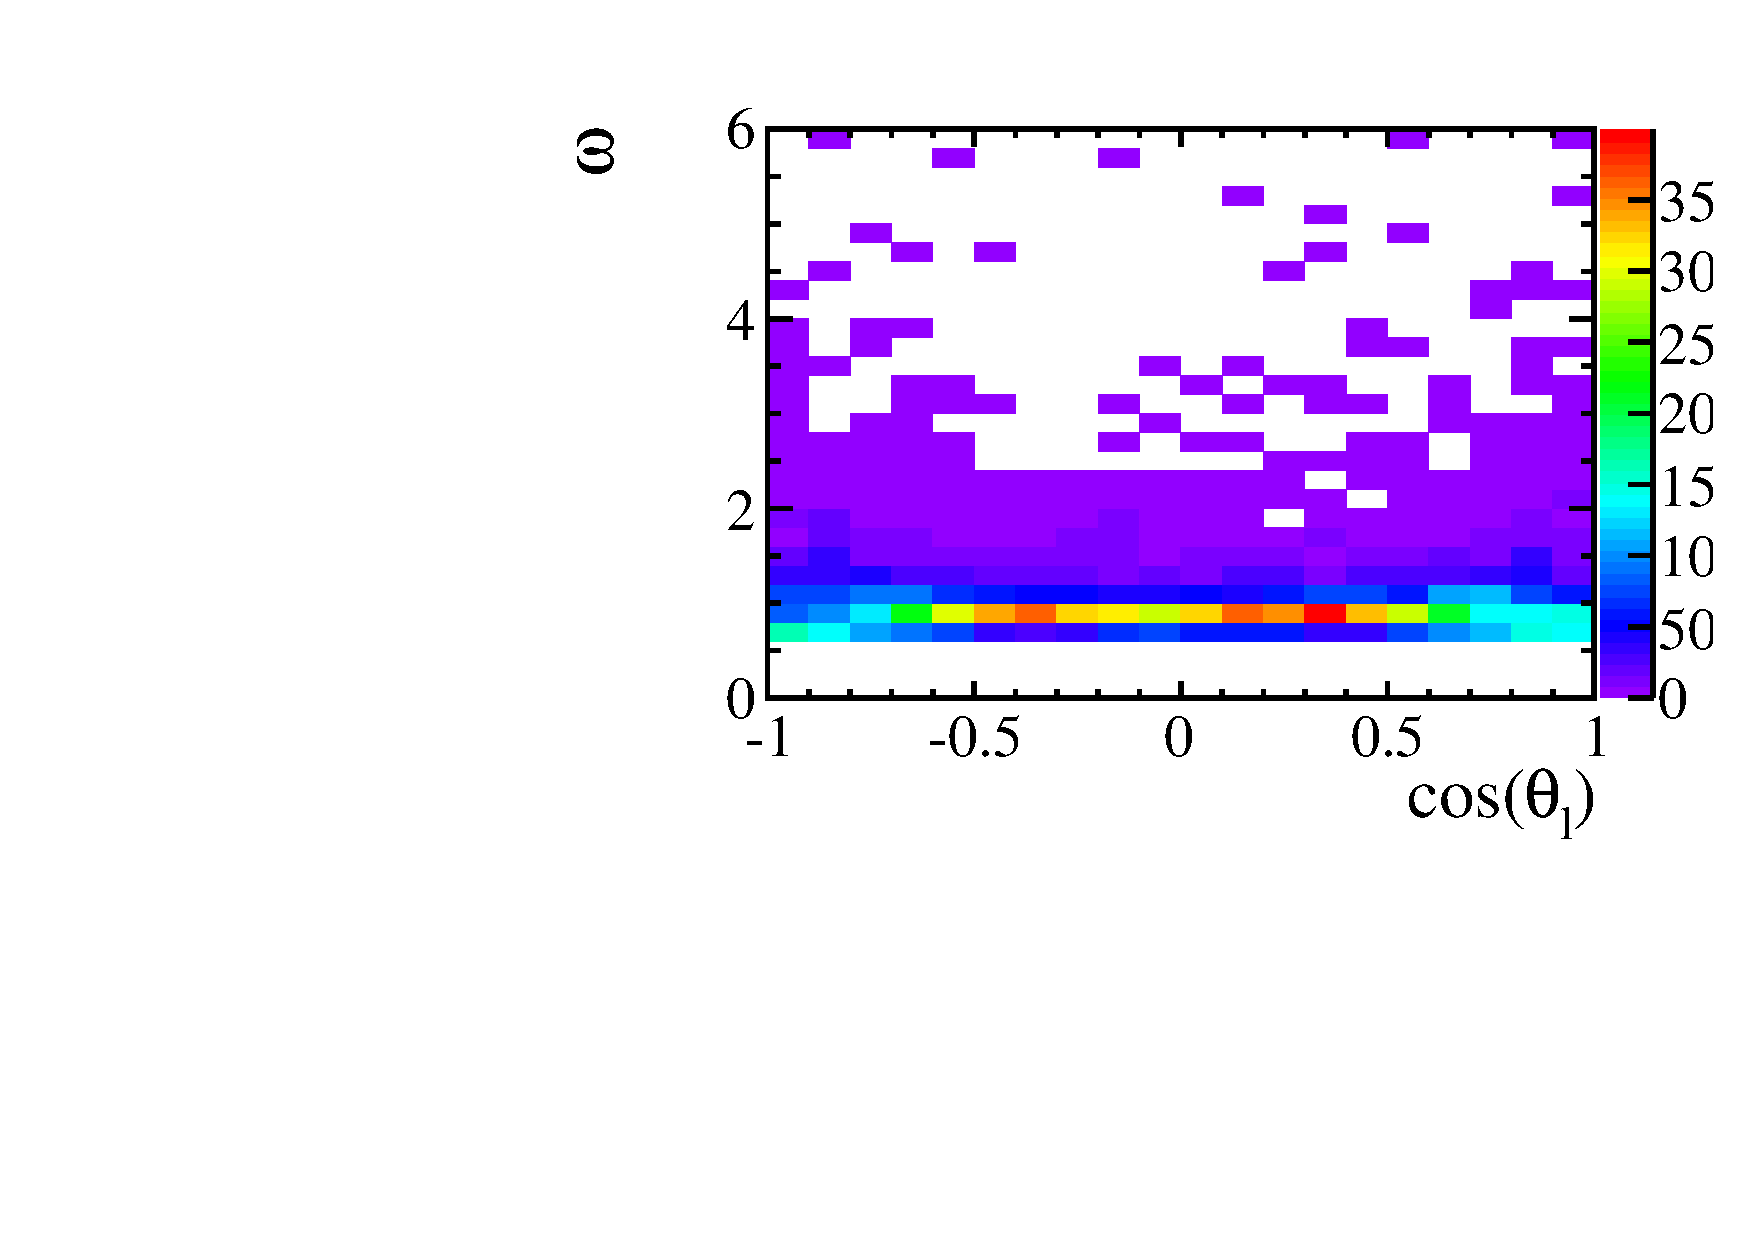
\includegraphics[width=0.48\columnwidth]{chapter5/figs/ac2/phasespace_weight_ctl.pdf}}
\subfigure[]{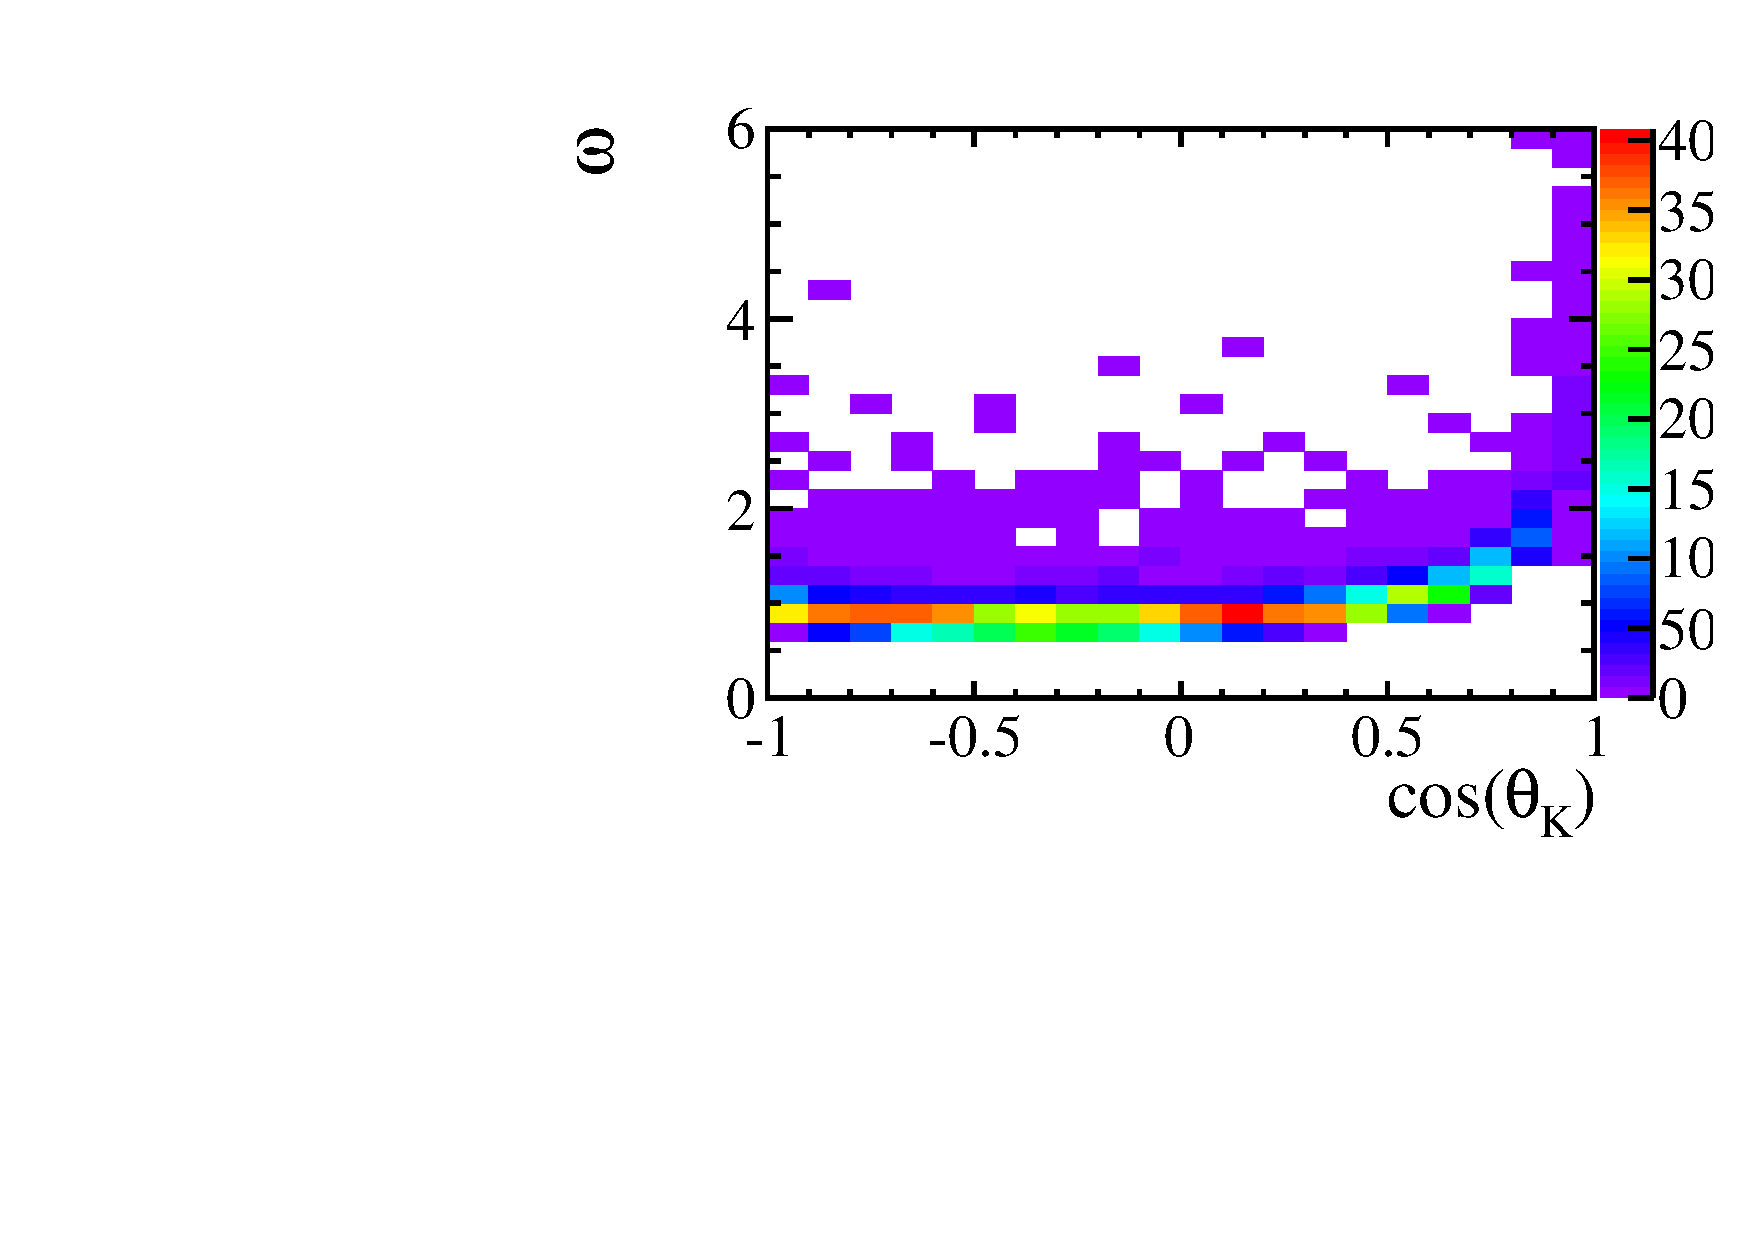
\includegraphics[width=0.48\columnwidth]{chapter5/figs/ac2/phasespace_weight_ctk.pdf}}
%\subfigure[]{\includegraphics[width=0.48\columnwidth]{chapter5/figs/ac2/phasespace_weight_phi.pdf}}
\caption[ The distribution of weights for 10000 phase space simulated \BdToKstmm events.] 
{ The distribution of weights for 10000 phase space simulated \BdToKstmm events and the correlation between 
the weights and \ctl and \ctk. The weights are normalised such that the sum of weights is equal to the 
number of events. The high weights for extreme \ctk and \ctl can be seen. ~\label{fig:ac2weights} }
\end{figure}
The larger weights for extreme \ctl and \ctk regions can be seen.% along with a small variation in \varphi.

\subsubsection{Testing the factorisation}
\label{sec:kstmm:facac:nonfac}

The assumption that the efficiency can be factorised is tested and 
the quality of the fit are assessed by using a variation of the binned $\chi^2$ test.
This modified test compares the distribution of data events used to fit a \PDF to the 
distribution of toy Monte Carlo events generated from the fitted \PDF.
The number of toy Monte Carlo events generated from the fitted \PDF 
using an accept/reject method was scaled to one hundred times the number of data events.
The phase space of \ctl, \ctk and $\phi$ was divided up into one thousand bins.
The pull value for each bin is calculated from
\begin{align}
p^i = n^{i}_{Data} - \left(\frac{n_{Data}^i - 10^{-2} n^{i}_{MC} }{ \sigma }\right)
\end{align}
where the error is defined as
\begin{align}
\sigma = \sqrt{( n_{Data}^i + 10^{-2} n_{MC} )} \, .
\end{align}
If the \PDF is a good fit to the data then the pull values should be normally distributed.
Here the `data' is the offline selected sample of phase space \BdToKstmm simulated events. 
Pull distributions for one low and one high \qsq bin are shown in Fig.~\ref{fig:facpulldist}.
\begin{figure}[tbp]
\centering
\subfigure[]{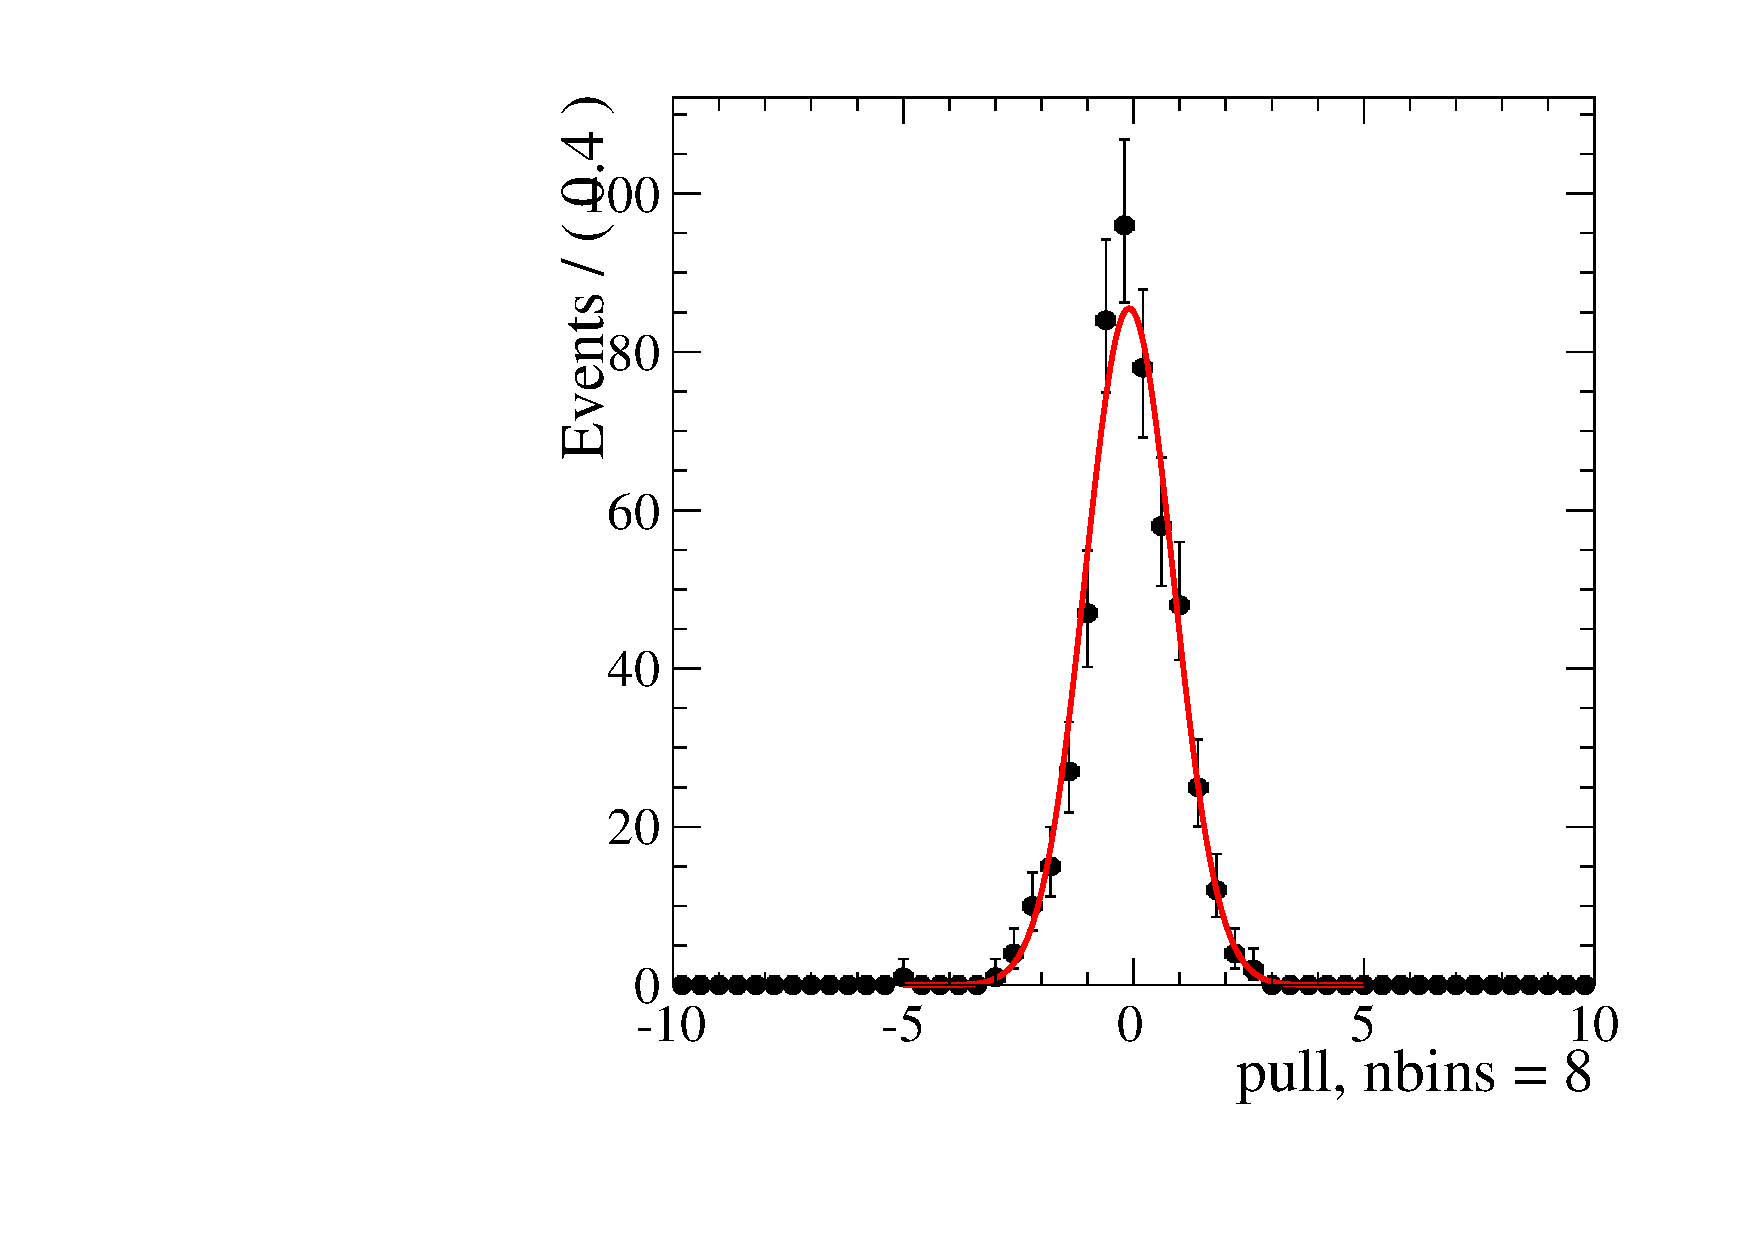
\includegraphics[width=0.48\columnwidth,page=1]{chapter5/figs/pull_dist_qsq_bins.pdf}}
\subfigure[]{\includegraphics[width=0.48\columnwidth,page=50]{chapter5/figs/pull_dist_qsq_bins.pdf}}
\caption [ The pull distribution of a toy simulation from the factorised \PDFs.] 
{ The pull distribution of a toy simulation from the factorised \PDFs.
A low \qsq bin (a) ($1<\qsq<2\gevgevcccc$) and a high \qsq bin (b) ($15<\qsq<15.5\gevgevcccc$). 
The fit for both distributions is compatible with a Gaussian of zero mean and unit width. ~\label{fig:facpulldist} }
\end{figure}
Both pull distributions are compatible with a Gaussian with zero mean and unit width.
The mean and width of the pull distribution for each bin in \qsq are given in Fig.~\ref{fig:facpulldistall}.
\begin{figure}[tbp]
\centering
\subfigure[]{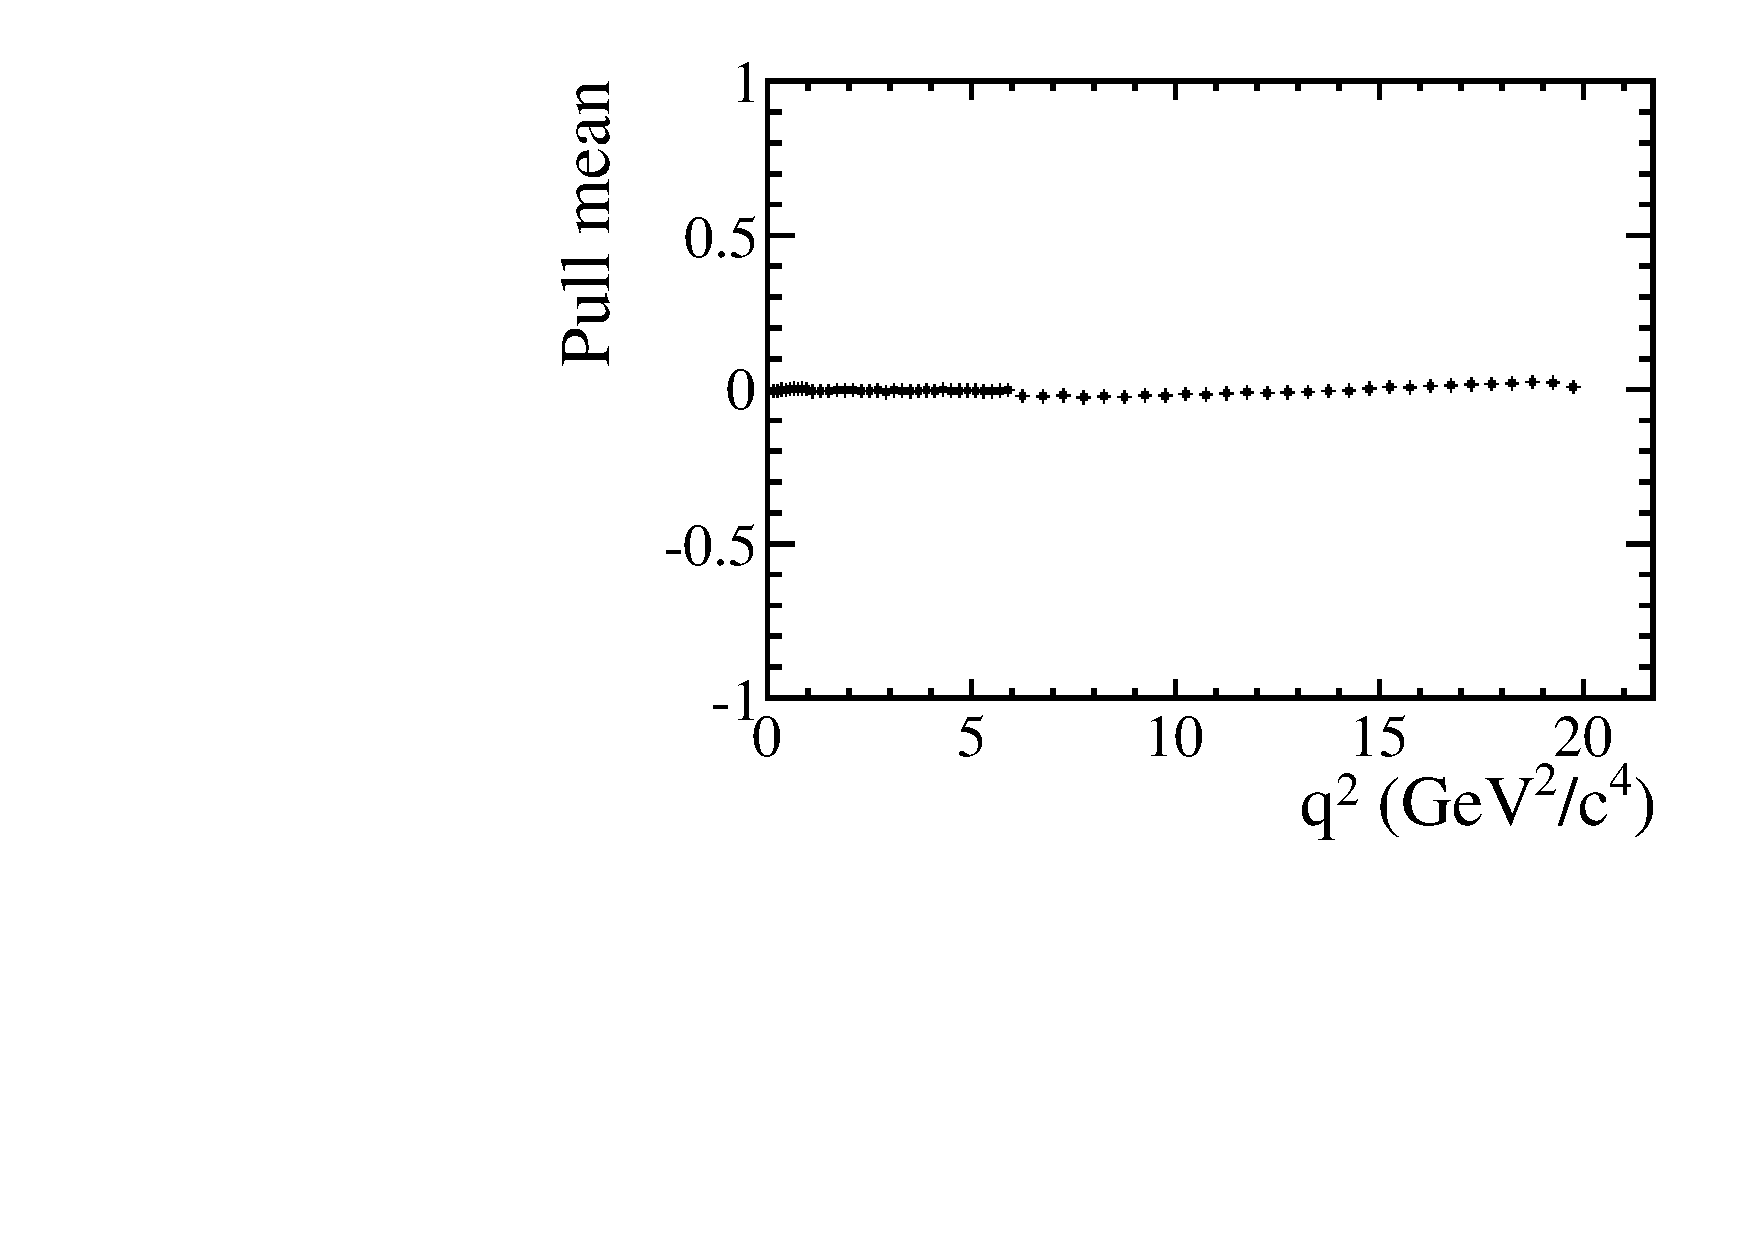
\includegraphics[width=0.48\columnwidth]{chapter5/figs/ac2/fiteff_results_62_pull_meangraph.pdf}}
\subfigure[]{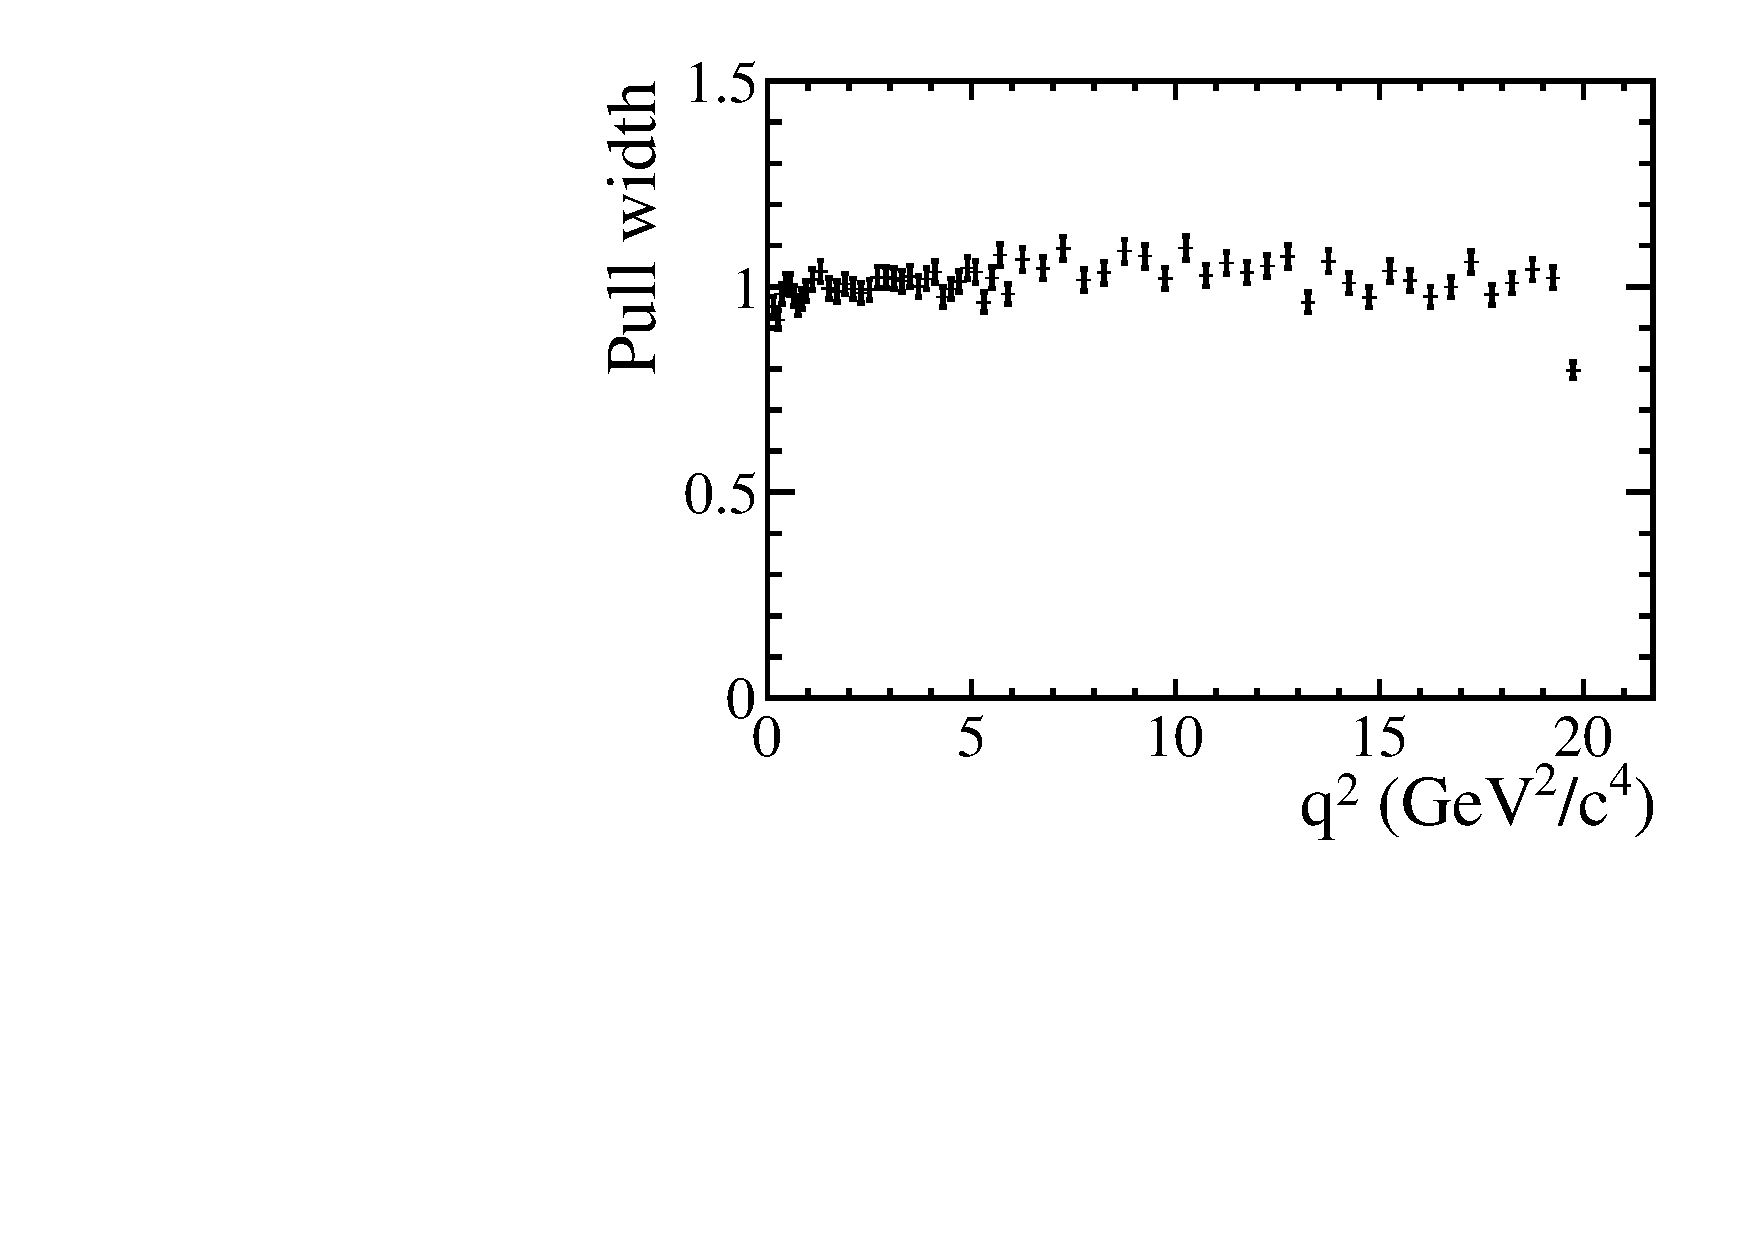
\includegraphics[width=0.48\columnwidth]{chapter5/figs/ac2/fiteff_results_62_pull_pullgraph_new.pdf}}
\caption [ The pull distribution of a toy simulation from the factorised \PDFs.] 
{ The (a) mean and (b) width of each pull distribution of a toy simulation from the factorised \PDFs in bins of \qsq.
The bins are all compatible with a Gaussian of zero mean and unit width. ~\label{fig:facpulldistall} }
\end{figure}
This shows that there are no regions of great discrepancy between the simulation and the factorised \PDF in these bins of \qsq.

The factorisation of the efficiency allows for a more precise acceptance correction at the cost of incurring a 
possible source of systematic uncertainty associated with integrating over non-factorisable effects.
The factorisation was also tested by comparing the re-weighted phase space simulated events to the 
generator level distributions in each of the factorised dimensions.

%The degree to which non-factorisable effects can be ignored is tested by
%multiplying the efficiency function with a non-factorisable function,
%\begin{align}
%f(\ctl,\ctk) = 1 + \alpha\sin(\pi\ctl)\sin(\pi\ctk)
%\end{align}
%where $\alpha$ is a scaling factor. The efficiency function is modelled as
%\begin{align}
%\epsilon^{'}(\qsq,\ctl,\ctk,\phi)_{(x<\qsq<y)} = \epsilon(\qsq,\ctl,\ctk,\phi)_{(x<\qsq<y)} \times f(\ctl,\ctk) \, .
%\end{align}
%The mean and width of a Gaussian fit to the pull distributions for various values of $\alpha$
%are shown in Fig.~\ref{fig:nonfactest}.
%\begin{figure}[tbp]
%\centering
%\dots
%\caption{ The pull mean and pull width for a Gaussian fit to the pull distribution between simulation and 
%toy Monte Carlo generated from the fitted efficiency as a function of the non-factorisable 
%scaling factor, $\alpha$. ~\label{fig:nonfactest} }
%\end{figure}

\subsection{Re-weighted phase space distributions}

The most basic test of an acceptance correction is that the original generator 
level distribution used to create the acceptance correction can be recovered.
In this case the phase space distribution %given in Fig.~\ref{fig:phsp}
should be recovered when the phase space candidates are themselves weighted.
The number of re-weighted \BdToKstmm candidates per bin in phase space is given by 
\begin{align}
N_{\text{bin}} = \sum_{i=1}^{ncand} \frac{1}{\epsilon(\ctl,\ctk,\phi)_i} = \sum_{i=1}^{ncand} \omega_i .
\end{align}
which can be compared to the expected number of generator level events in that bin. 

The weighted distributions for the $k$-nearest-neighbour acceptance correction method are shown in
Fig.~\ref{fig:corrphsp1}.
\begin{figure}[tbp]
\centering
\subfigure[]{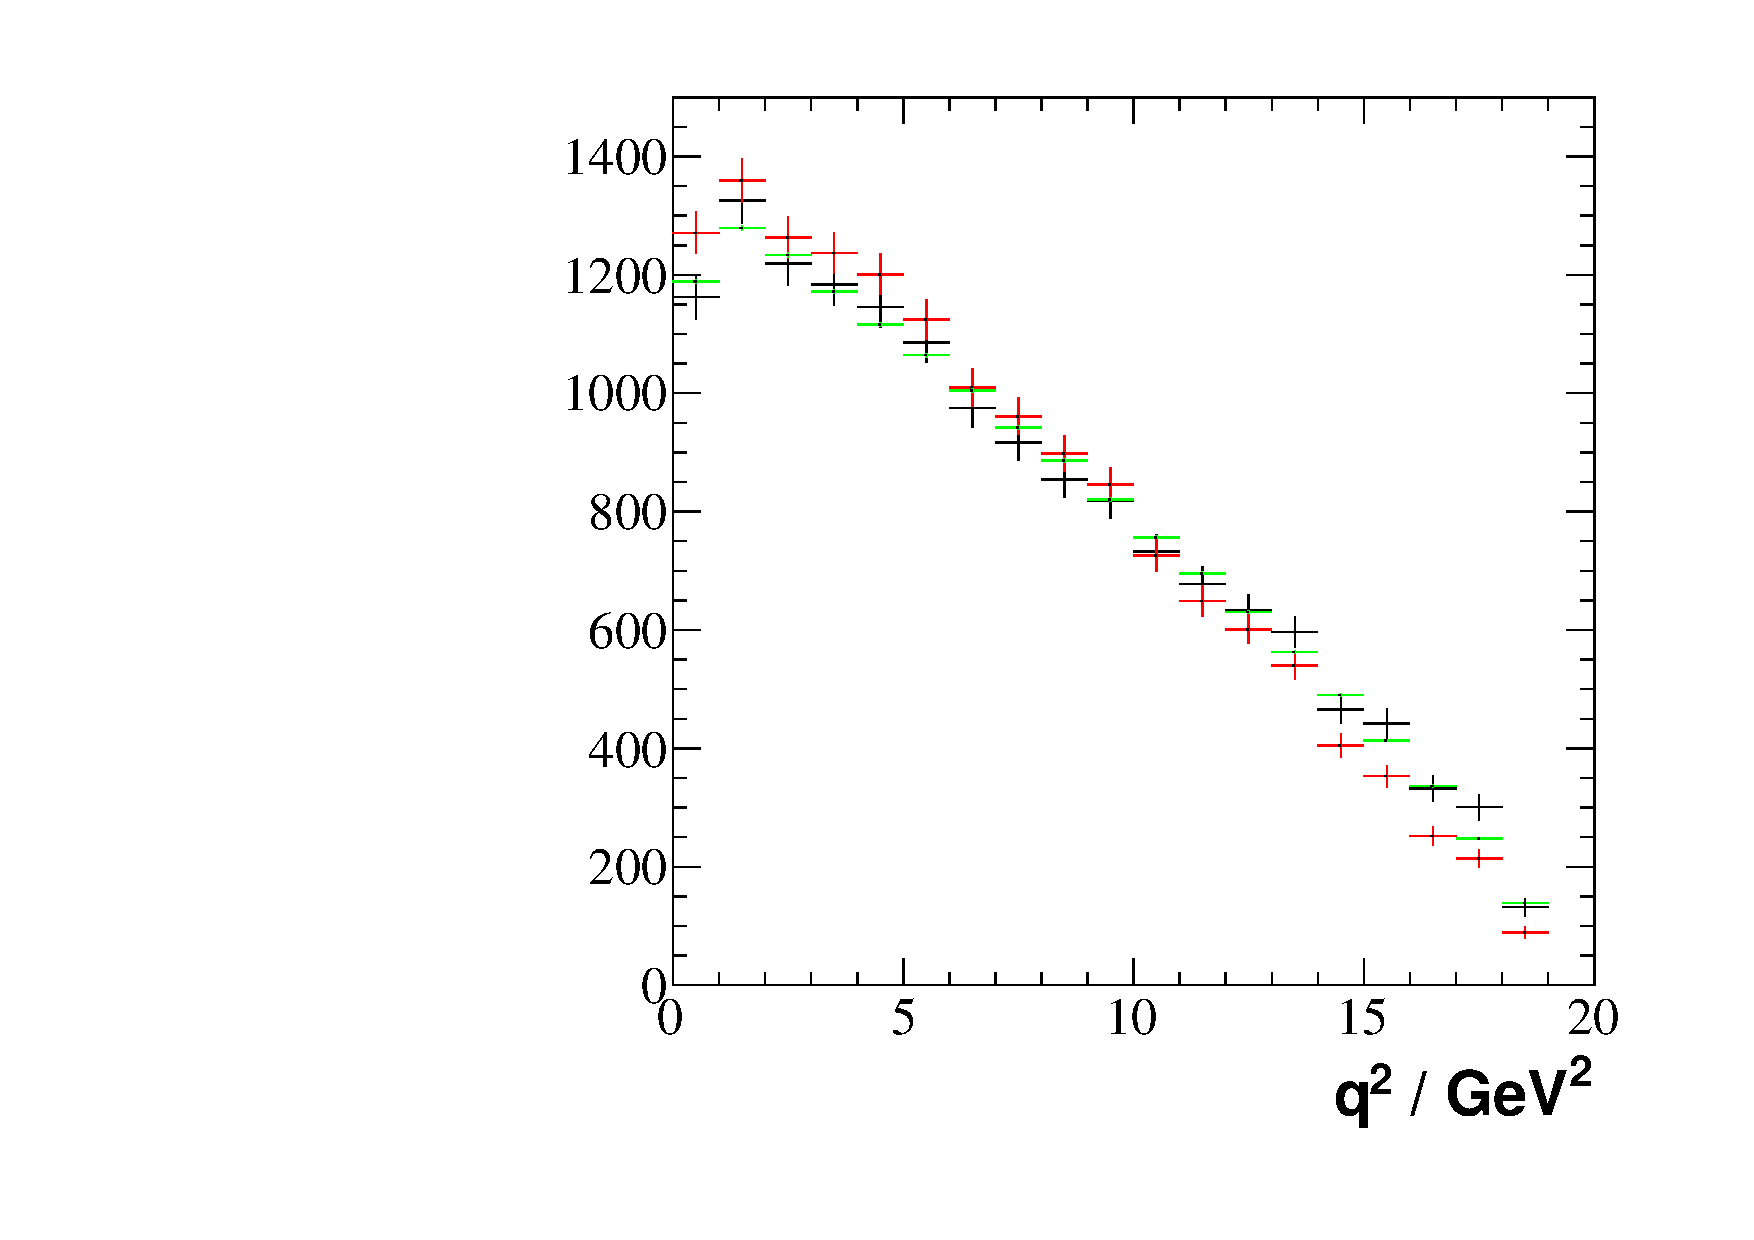
\includegraphics[width=0.32\columnwidth]{chapter5/figs/ac1/CorrectionsWithGen_Qsquare.pdf}}
\subfigure[]{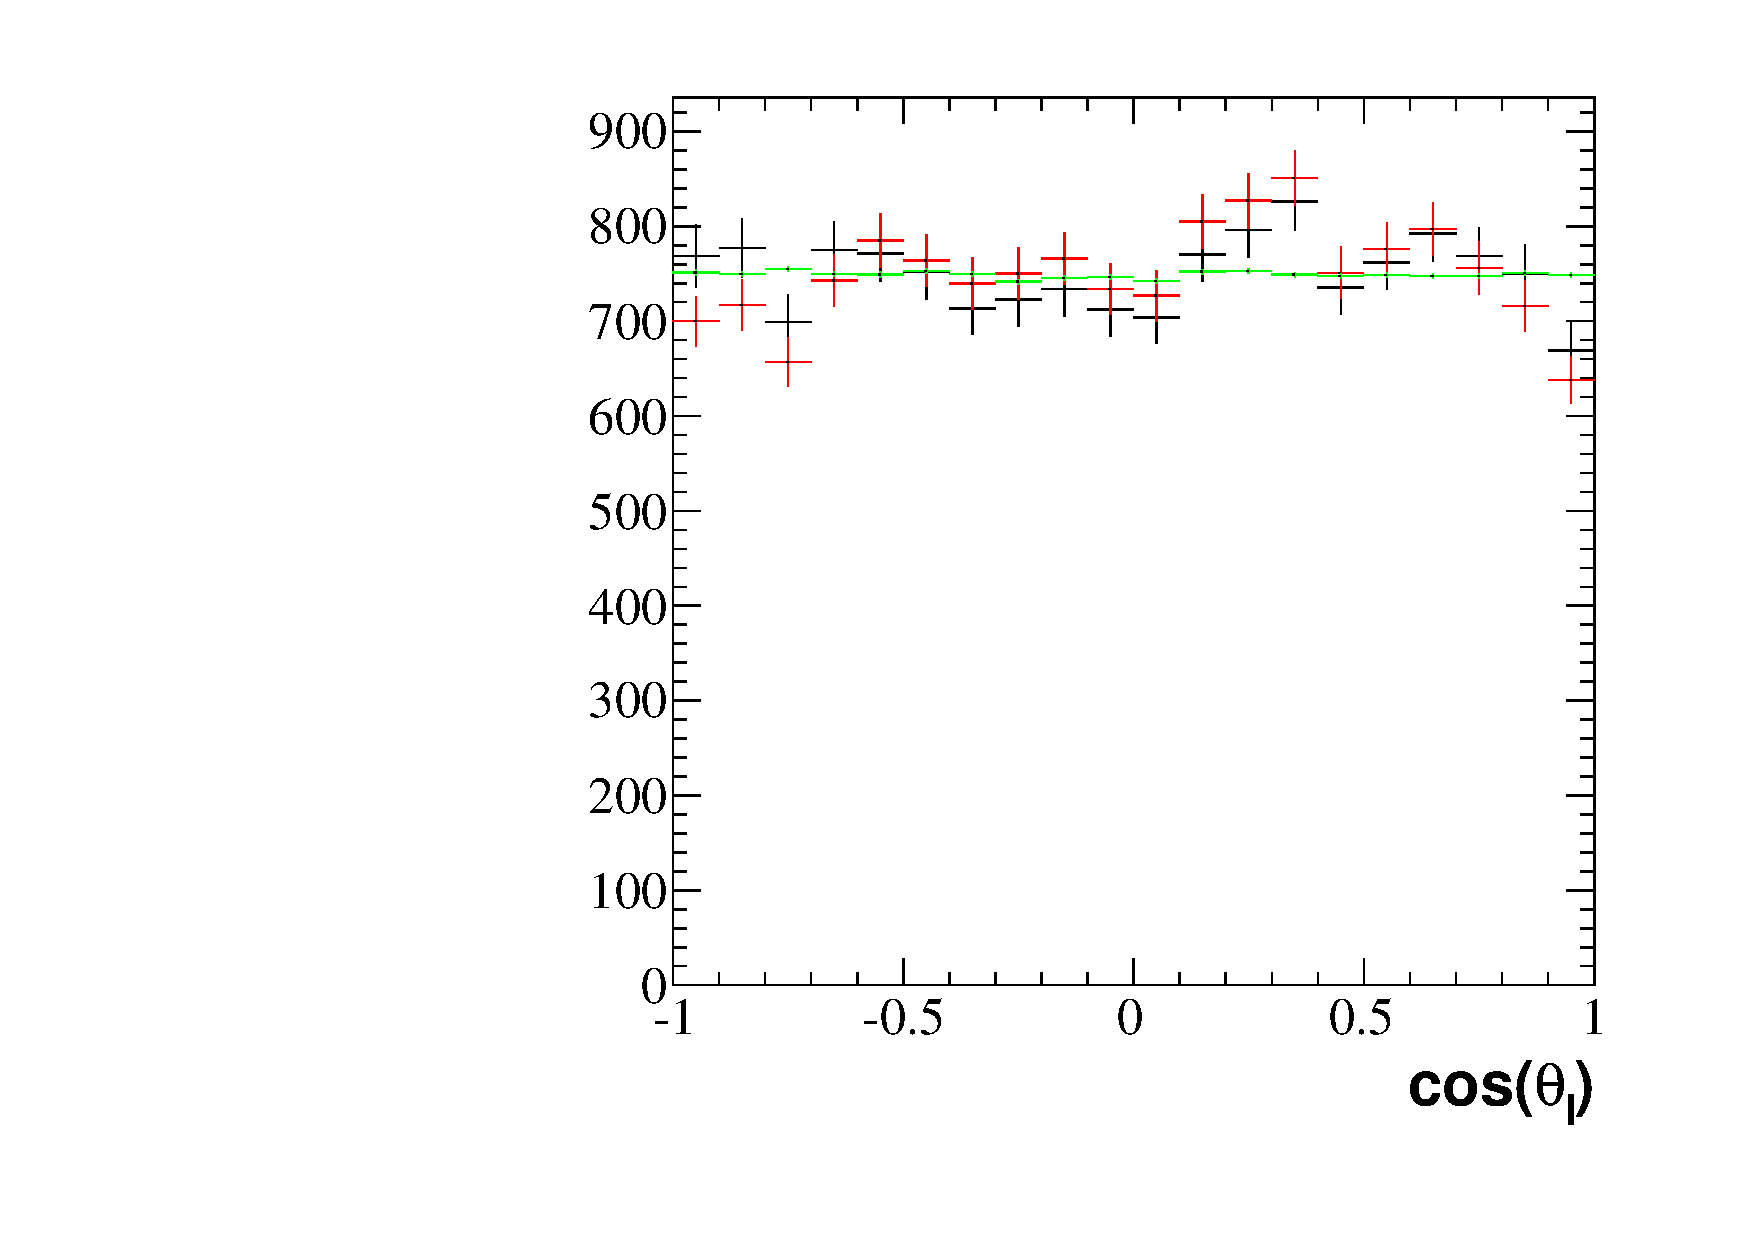
\includegraphics[width=0.32\columnwidth]{chapter5/figs/ac1/CorrectionsWithGen_ThetaL.pdf}}
\subfigure[]{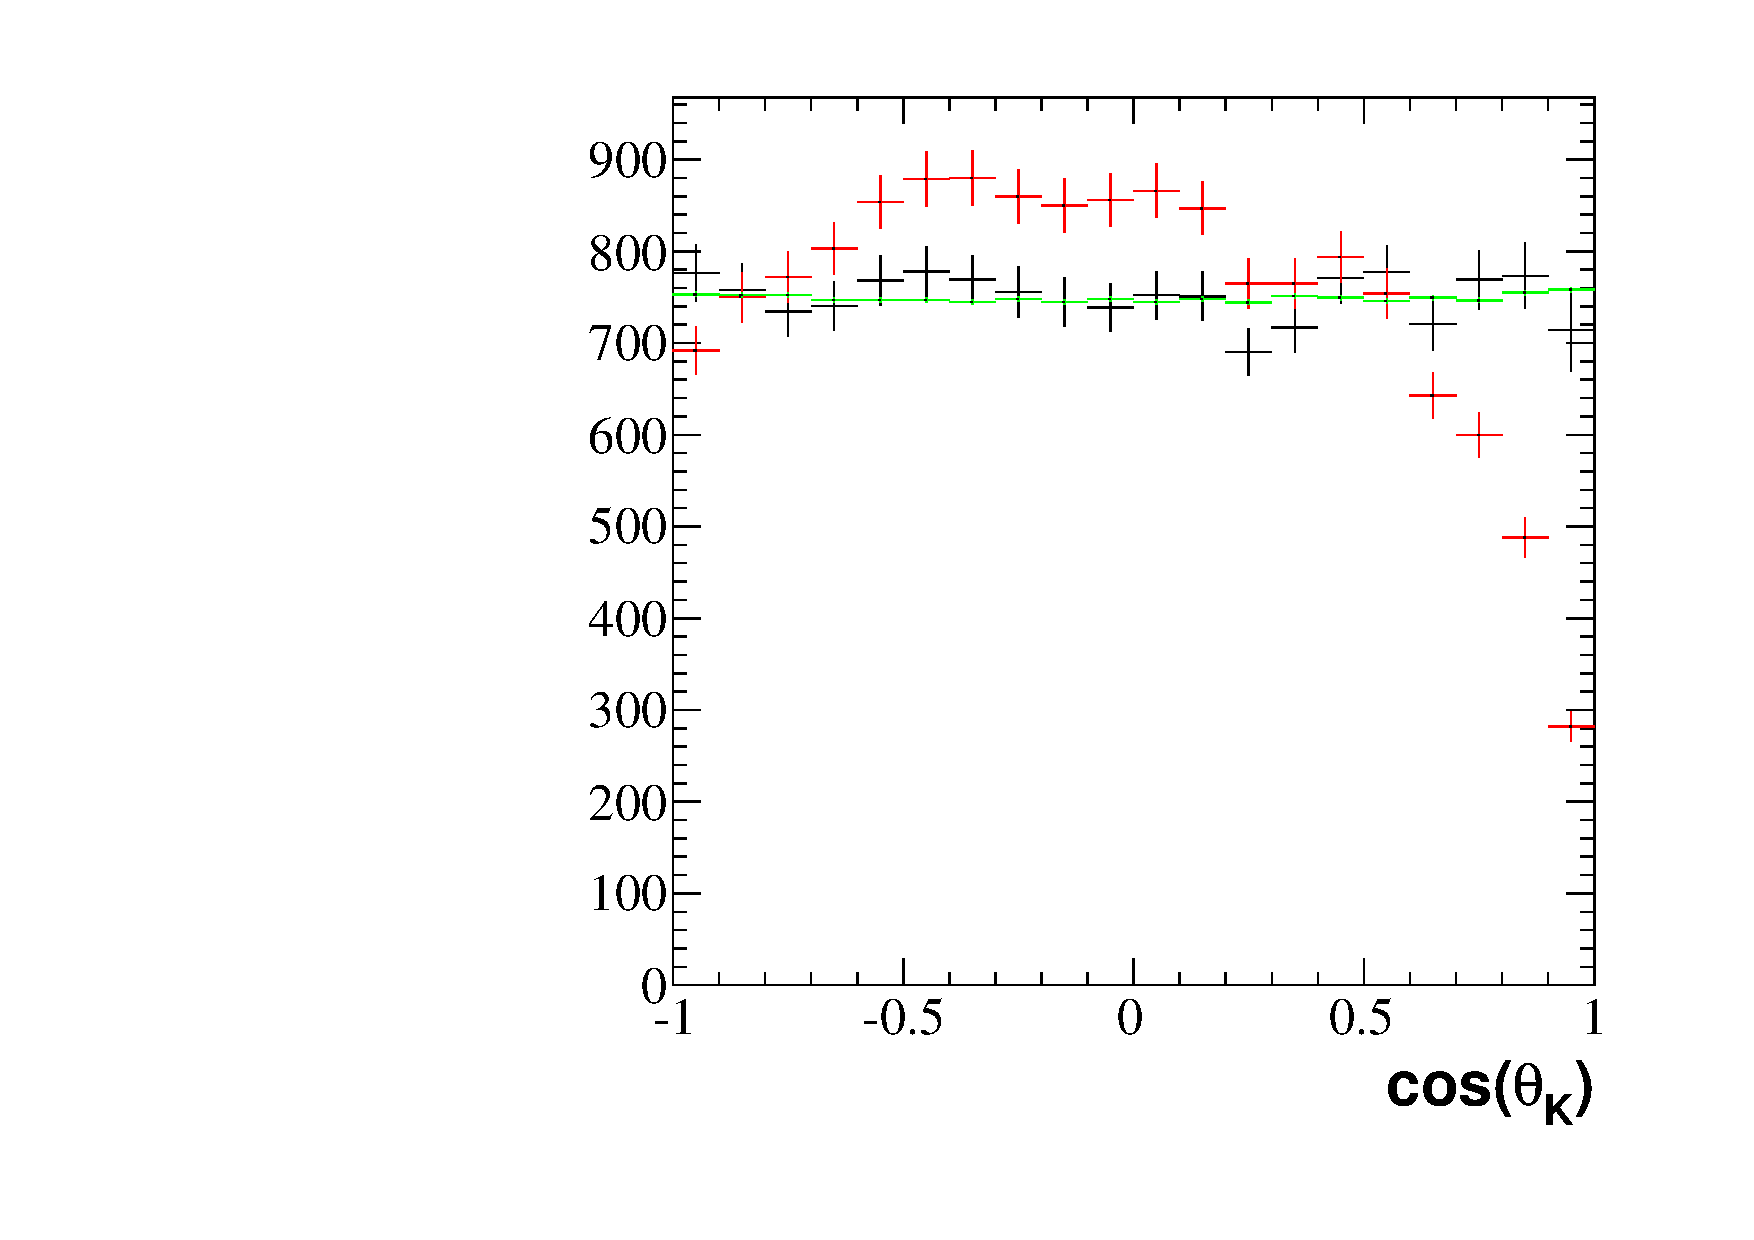
\includegraphics[width=0.32\columnwidth]{chapter5/figs/ac1/CorrectionsWithGen_ThetaK.pdf}}
\caption{Generated (green), offline selected (red) and re-weighted (black) events for  \BdToKstmm using the 
$k$-nearest-neighbour acceptance correction method.~\label{fig:corrphsp1}}
\end{figure}
Is it possible to see that the efficiency at extreme \ctk and extreme \ctl is recovered. 

The weighted distributions for the factorised acceptance correction method are shown in Fig.~\ref{fig:corrphsp2}.
\begin{figure}[tbp]
\centering
\subfigure[]{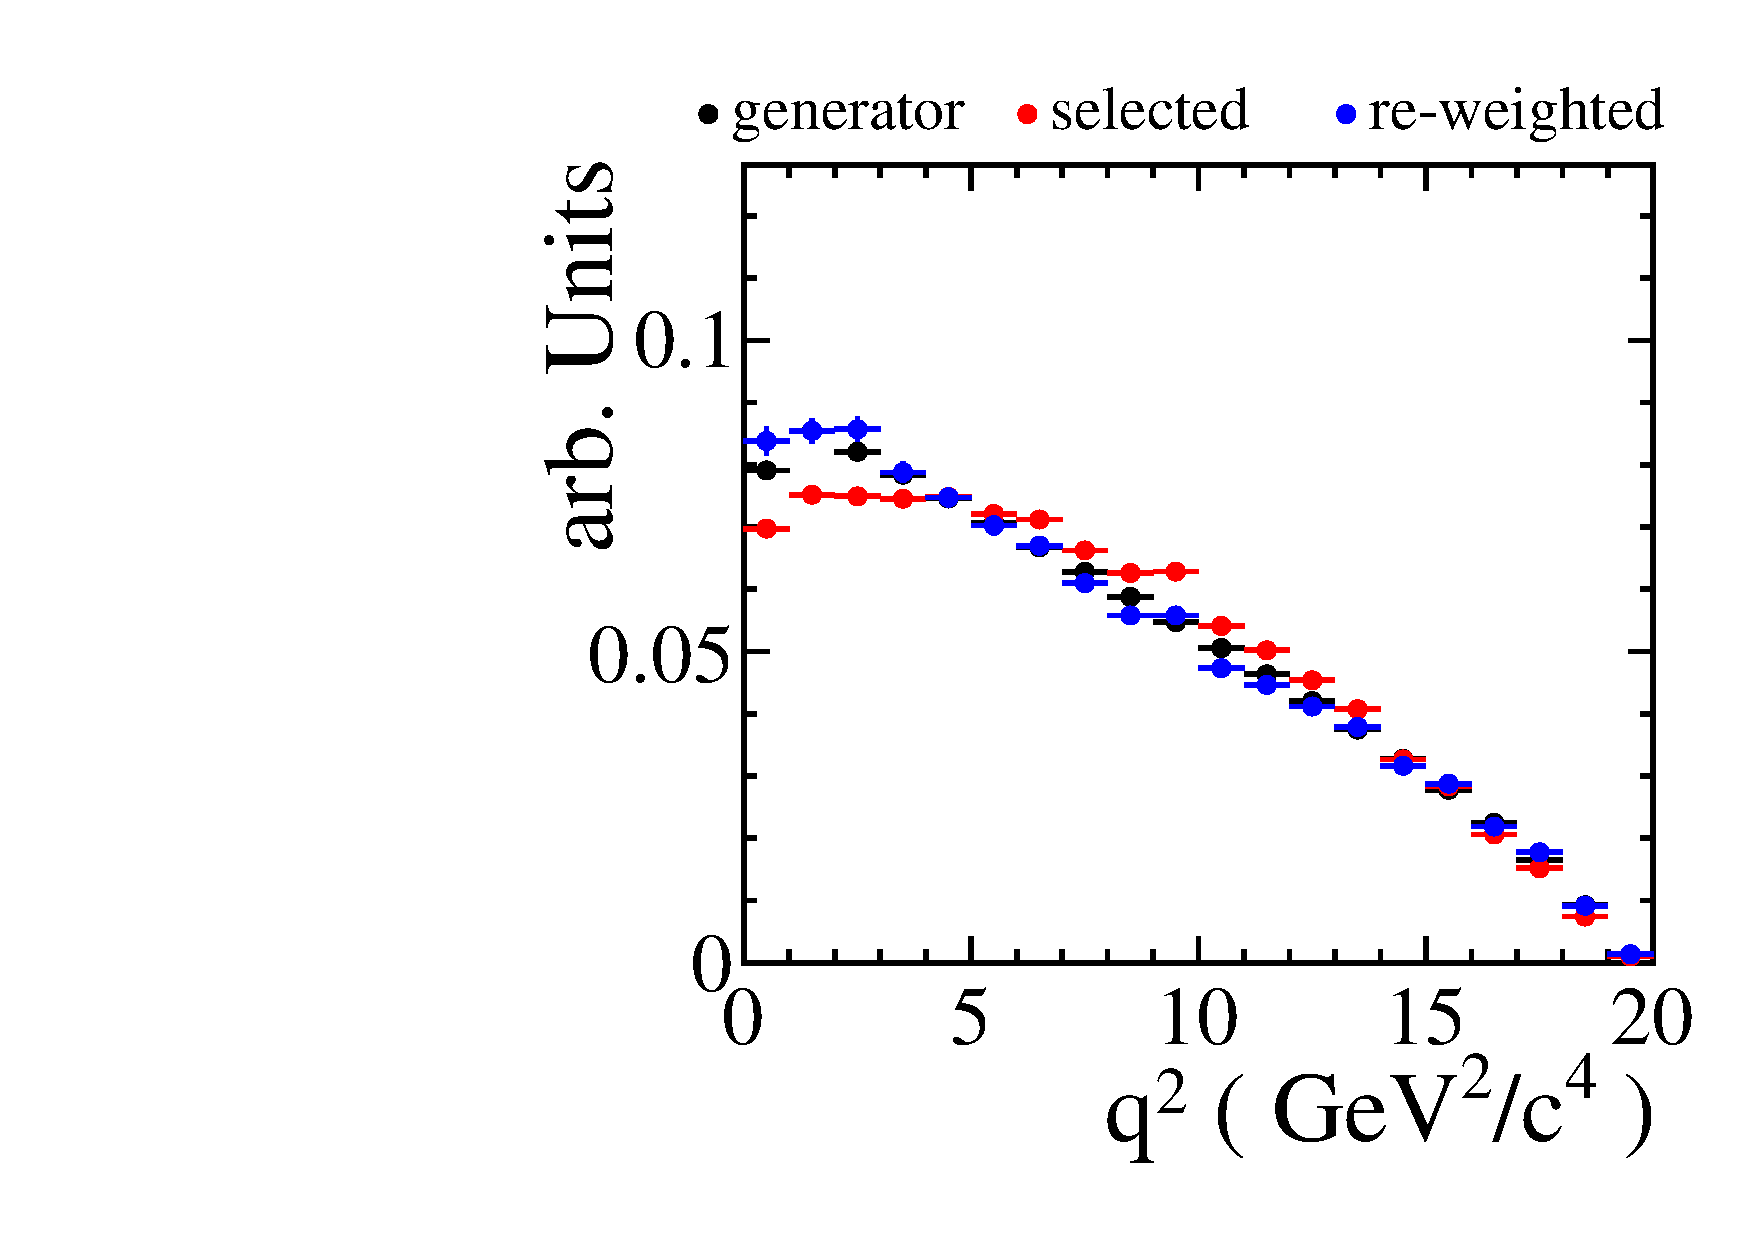
\includegraphics[width=0.48\columnwidth]{chapter5/figs/ac2/CorrectionsWithGen_Qsquare_new.pdf}}
\subfigure[]{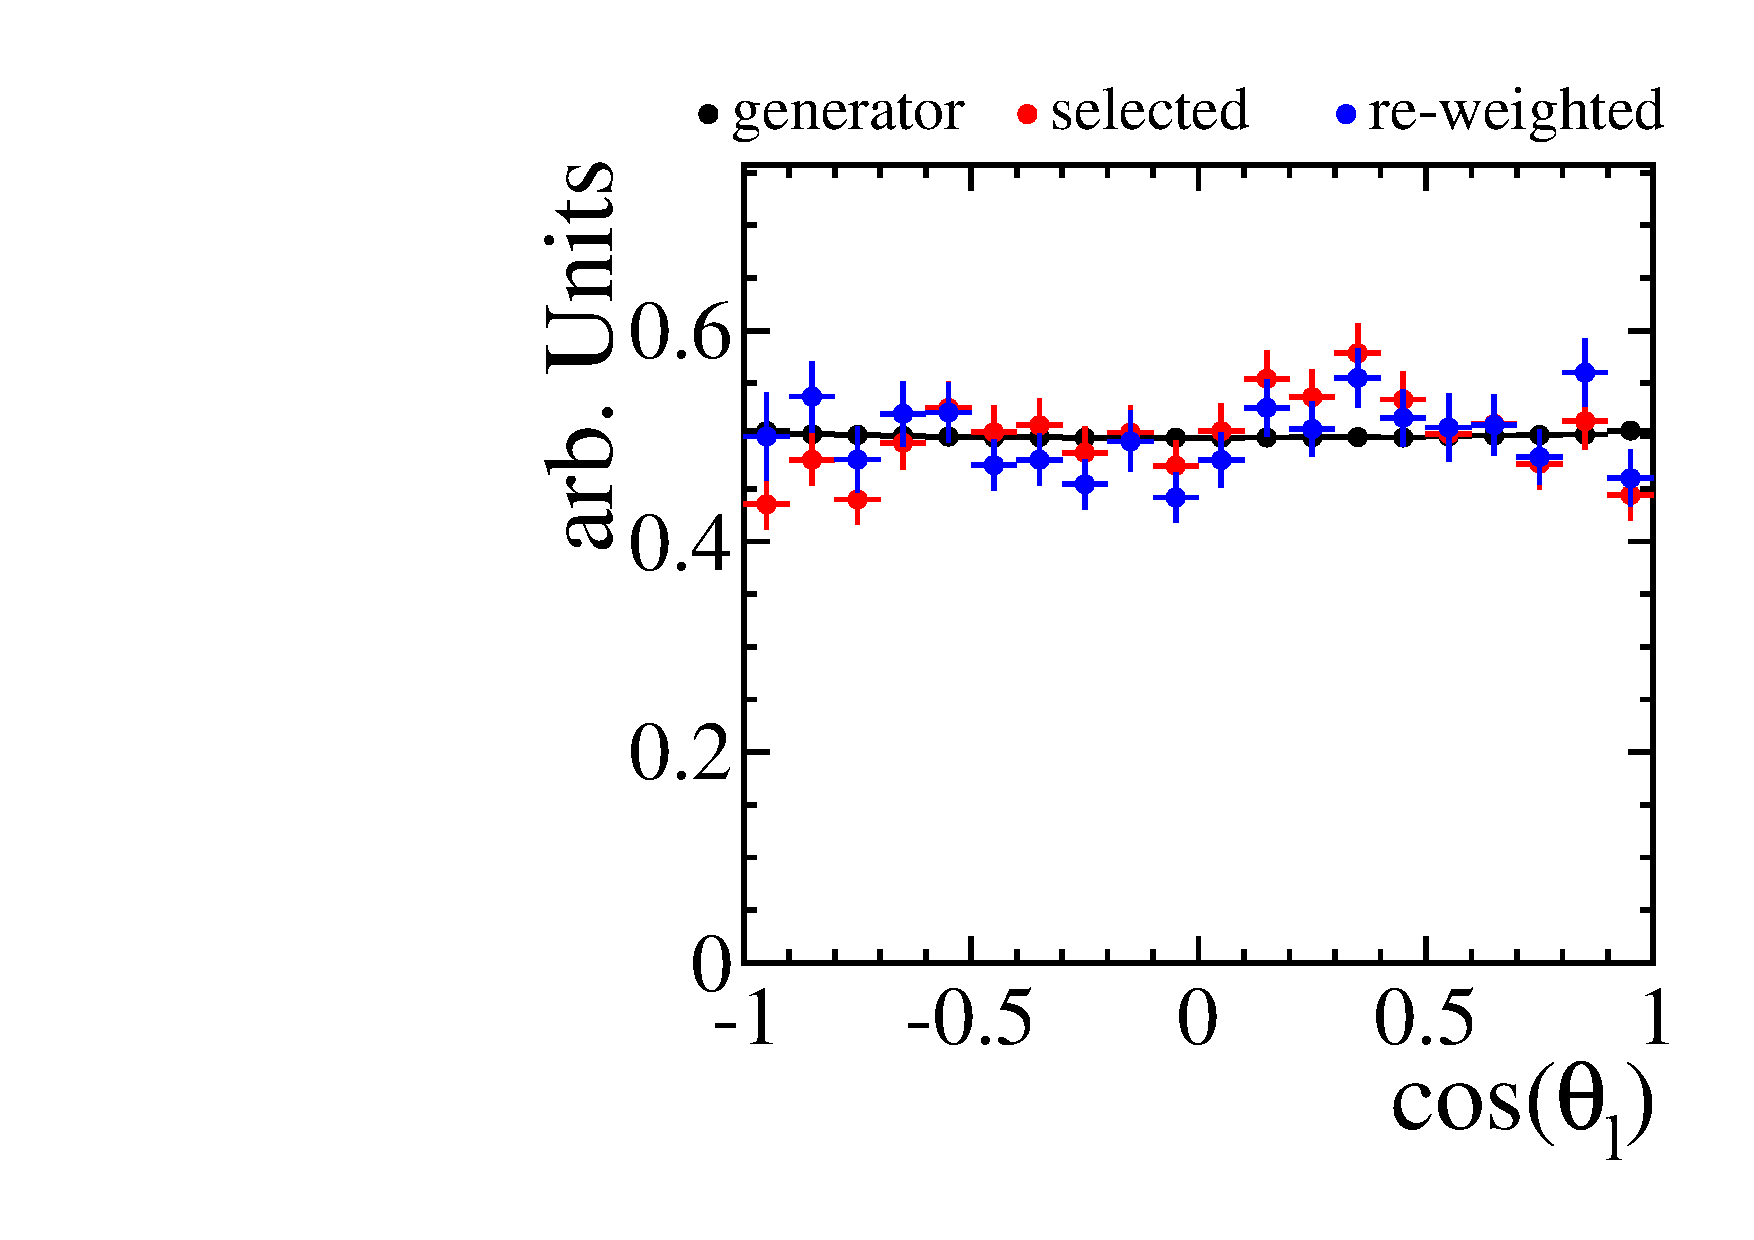
\includegraphics[width=0.48\columnwidth]{chapter5/figs/ac2/CorrectionsWithGen_ThetaL_new.pdf}}
\subfigure[]{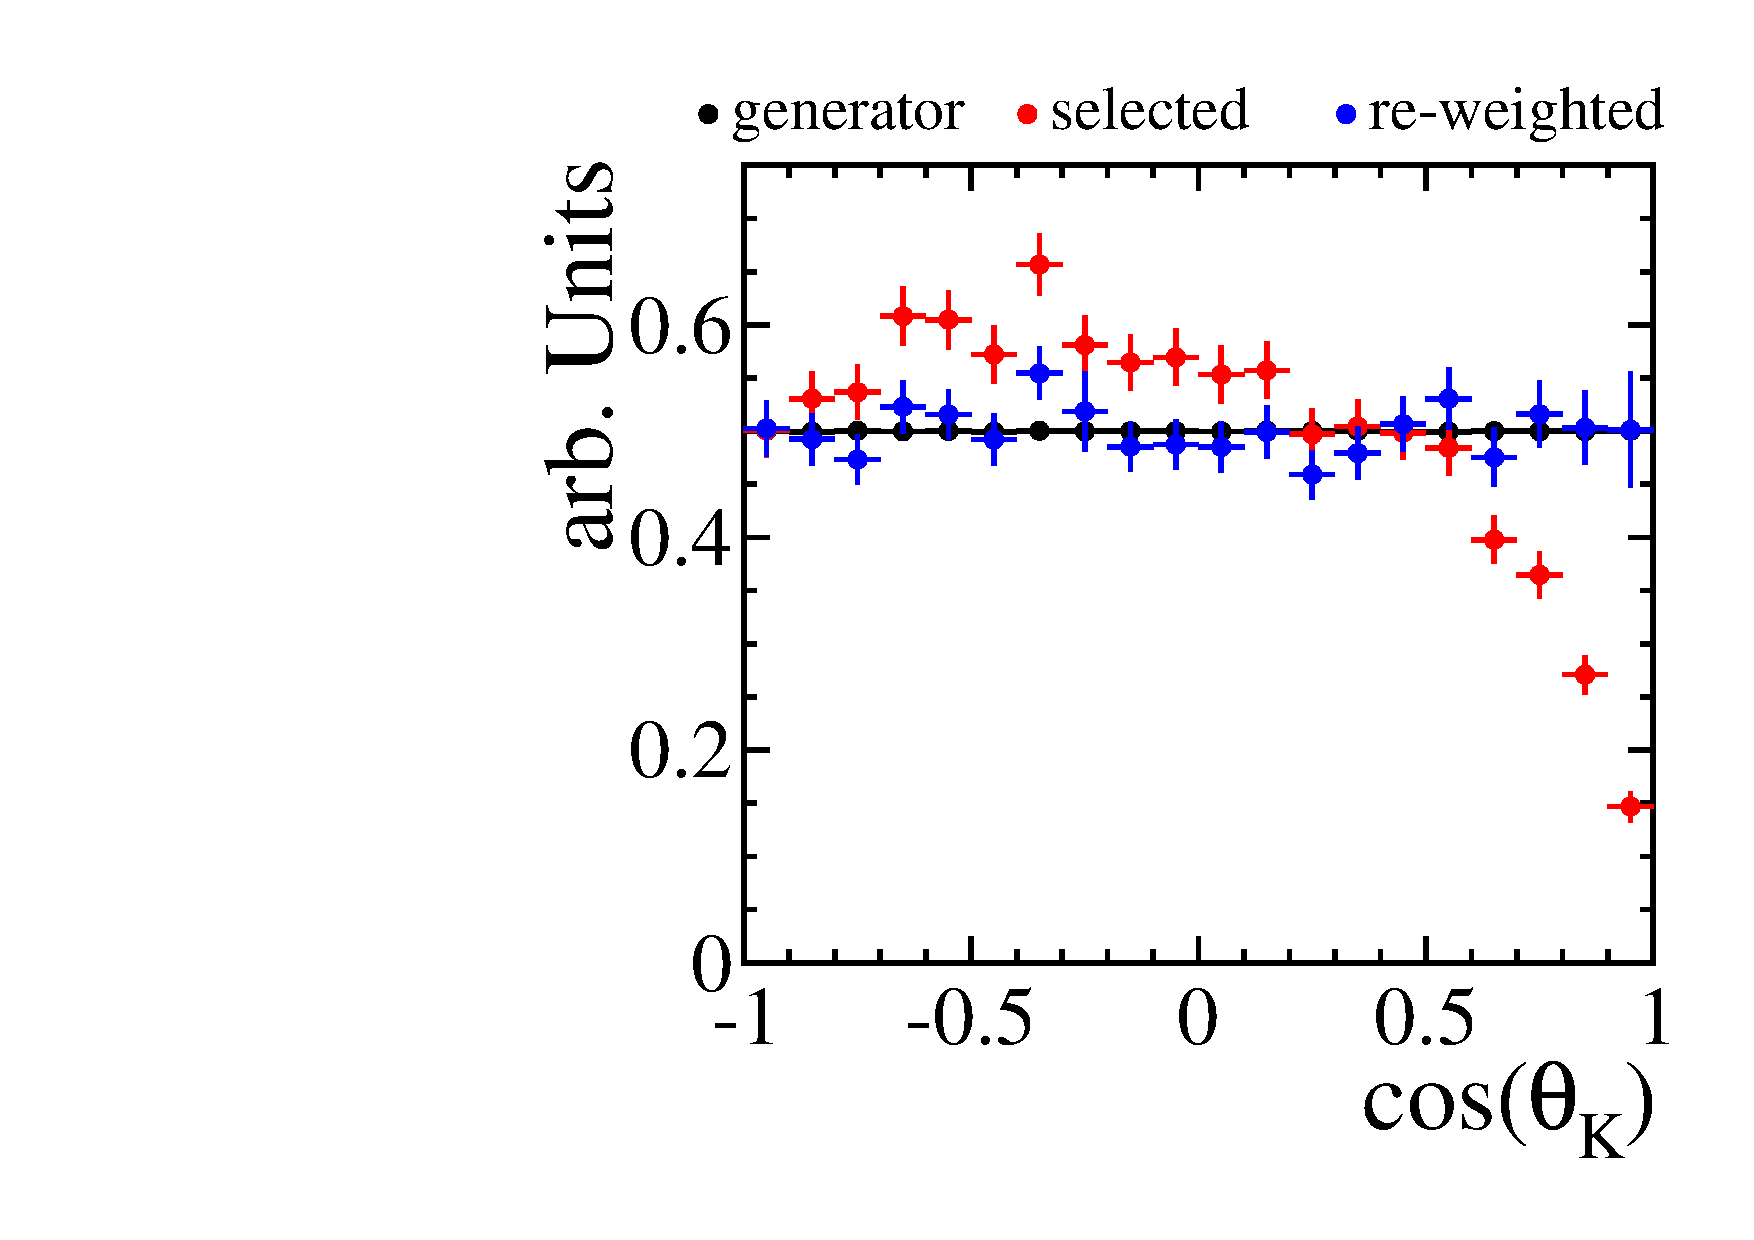
\includegraphics[width=0.48\columnwidth]{chapter5/figs/ac2/CorrectionsWithGen_ThetaK_new.pdf}}
\subfigure[]{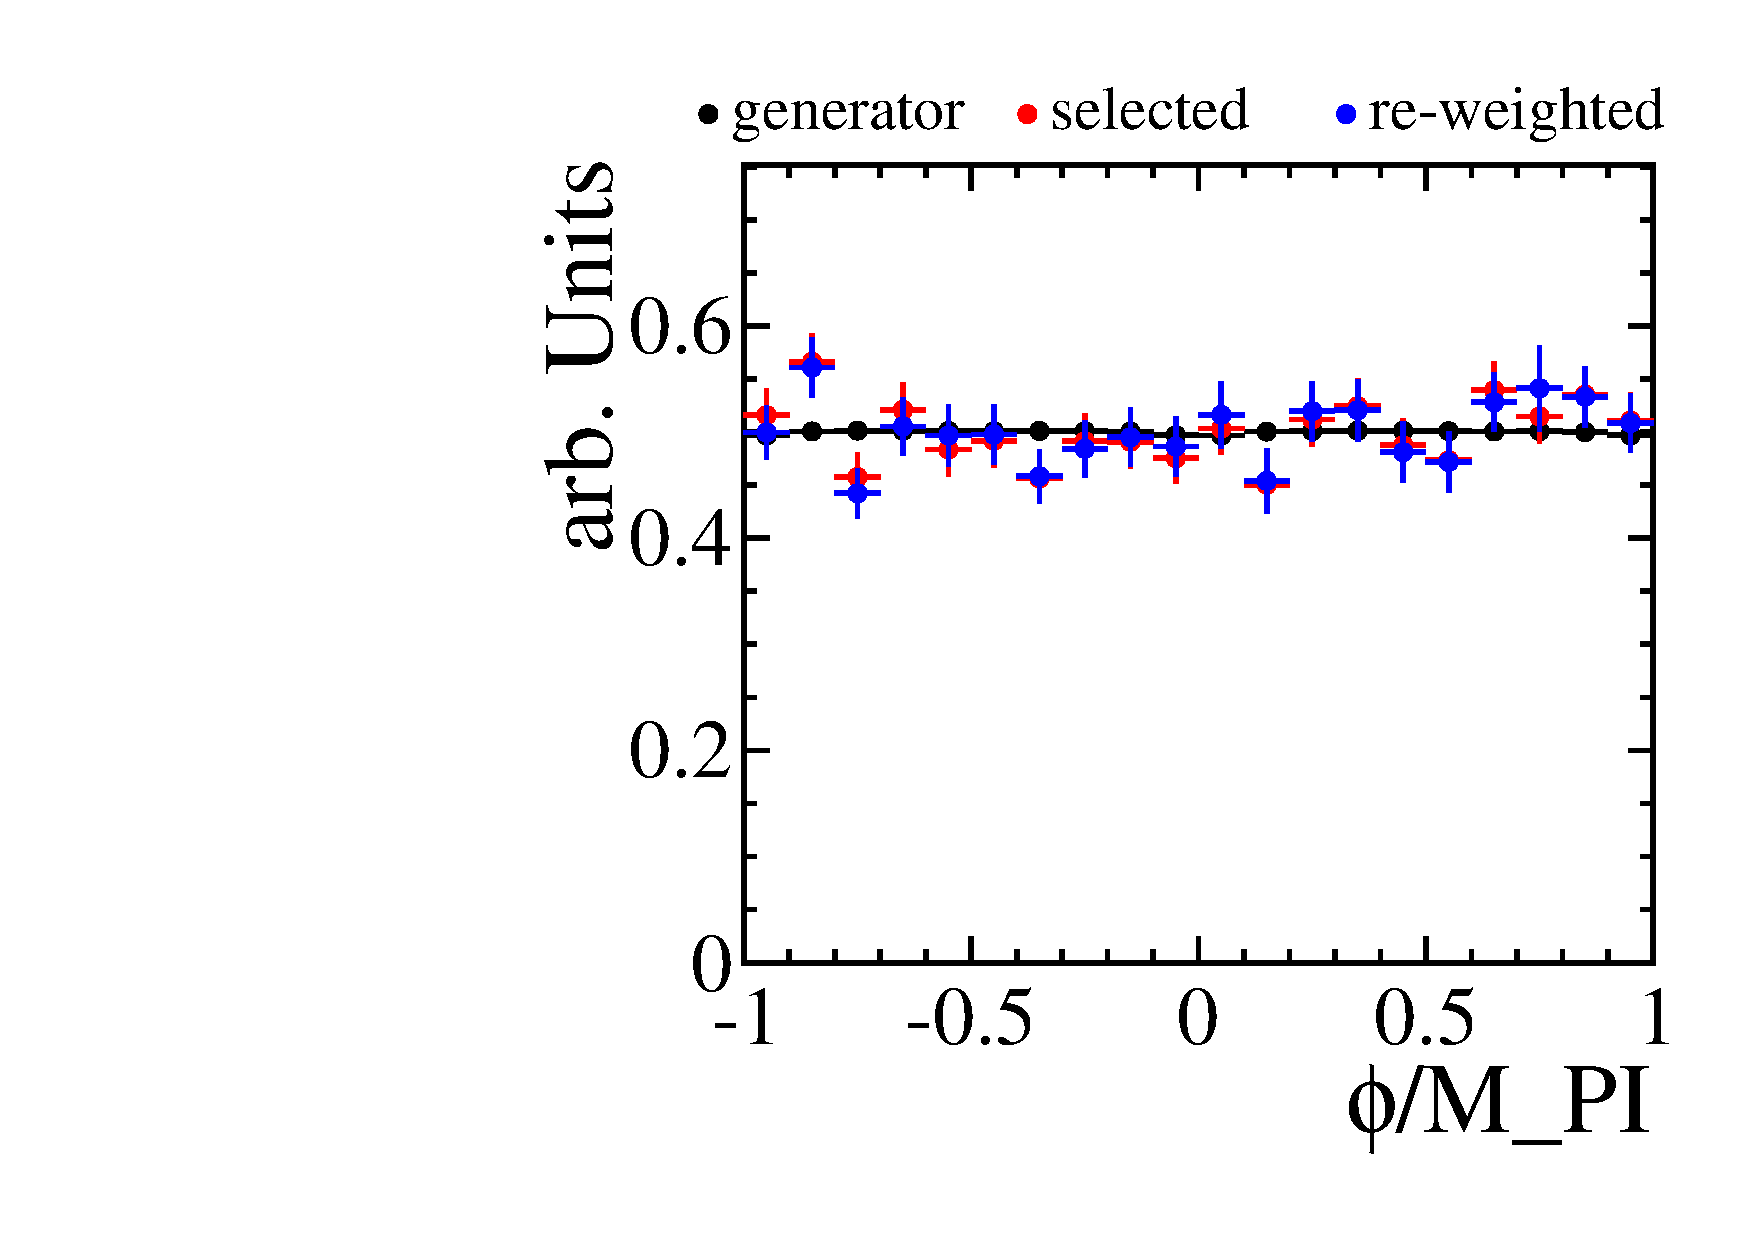
\includegraphics[width=0.48\columnwidth]{chapter5/figs/ac2/CorrectionsWithGen_Phi_new.pdf}}
\caption{Generated (black), offline selected (red) and re-weighted (blue) events for  \BdToKstmm using the factorised acceptance correction method.~\label{fig:corrphsp2}}
\end{figure}
The compatibility between the re-weighted distribution and the distribution  of generator level events 
is good for both acceptance correction methods.


The k-nearest-neighbour method is by construction the most optimal acceptance correction method as it relies only on the accuracy of the simulation
 from which to calculate the efficiency. 
However, the dependence on the simulation statistics in regions of phase
space with low efficiency does not allow it to be used with larger
datasets. The factorised efficiency correction has for the 1.0\invfb
analysis a lower total systematic error. The statistical component from
the simulation sample size is much smaller but the assumption of
factorisation incurs an additional but still small systematic uncertainty.



\section{Angular analysis}
\label{sec:kstmm:pdf}

Each of the angular analyses were performed by simultaneously fitting a \PDF for the mass and the angular distribution 
to the data. % the extended maximum likelihood fit method.
%The \PDF used is a combination of a model for the the \Bd mass spectrum and the angular \PDF.
The simultaneous fit to the \Bd mass spectrum and to the angles ensures that the
 maximum information available is used to reduce the error on all of the angular observables.
It also ensures that the correlations are propagated correctly between the angular observables.
The total \PDF ($F$) is a combination of a model for the signal ($S$) and background ($B$) ,
each containing component \PDFs to describe the mass distribution and the angular distribution,
\begin{align}
F(\mB, \ctl, \ctk, \phi) = & f_{sig} \left( S_{i}(\mB) \times S_{i}(\ctl,\ctk,\phi) \right) \nonumber \\ 
&+ ( 1 - f_{sig} ) \left( B_{i}(\mB) \times B_{i}(\ctl,\ctk,\phi) \right) \, .
\end{align}
where $i$ indicates the model used for the first or second analysis.
The different components of the total \PDF are described in detail below.

The dataset is divided into seven bins of \qsq.
 There are six separate bins in the full \qsq range, detailed in Table~\ref{tbl:qsqbins}.
\begin{table}
\centering
\caption[ The \qsq binning scheme used in both angular analyses. ]
{ The \qsq binning scheme used in both angular analyses. 
The binning is analogous to the binning used in Ref~\cite{PhysRevLett.103.171801} including
 the  \qsq region of 1 to 6 \gevgevcccc .~\label{tbl:qsqbins} }
\begin{tabular}{|c|c|}
\hline
lower limit (\gevgevcccc)  & upper limit (\gevgevcccc) \\
\hline
0.1 & 2 \\
2 & 4.3 \\
4.3 & 8.68 \\
10.09 & 12.9 \\
14.18 & 16 \\
16 & 19 \\
\hline
1.0 & 6.0 \\
\hline
\end{tabular}
\end{table}
The binning is analogous to the binning used in Ref~\cite{PhysRevLett.103.171801} along with the
 region from $1 < \qsq < 6 \gevgevcccc $, which is a theoretically clean region where the observables are easily calculable.
The binning is chosen such that there is a bin below and above the point where \AFB is
 predicted to change sign in the Standard Model, and also with boundaries to avoid the \ccbar resonances.

\subsection{Mass model}
\label{sec:kstmm:massmodel}

Two different mass models were used to parametrise the \Bd signal invariant mass distribution.
The signal invariant mass model used to parametrise the \Bd invariant mass distribution in the first angular analysis was a double Gaussian function,
\begin{align}
\label{eq:totpdf}
S_{(1)}\left( \mkpimm ; \sigma_1, \sigma_2, \alpha, n \right) = & \, f \times G\left(  \mkpimm  ; m_B , \sigma_1 \right) \nonumber\\
& + \left(1-f\right) \times G\left(  \mkpimm ; m_B , \sigma_2\right) \, ,
\end{align}
where $f$ is the fraction of signal between each component and $\sigma_{1,2}$ are the different widths of each Gaussian component.
The signal mass model for the second angular analysis was an empirical model consisting of two Crystal Ball functions.
The Crystal Ball was a function developed to model the radiative 
tail from the \bbbar resonances~\cite{Skwarnicki:1986xj}.
It consists of a Gaussian distribution with an 
exponential tail and is expressed for a given mass ( \mkpimm ) as
\begin{equation}
\CB \left(  \mkpimm ; \mB , \sigma, \alpha, n \right) = N
\begin{cases}
  \exp{\left(\frac{-(\mkpimm - \mB )^2 }{2\sigma^2}\right)} 
 & \text{if} \,\, \mkpimm >  \alpha  \\
 \frac{\left(\frac{n}{\alpha^2}\right)^n}{\frac{\left(\mkpimm-\mB \right)}{\sigma} + \frac{n}{\alpha} - \alpha }
 & \text{if} \,\, \mkpimm\leq  \alpha
\end{cases}
\end{equation}
where $N$ is the signal normalisation, \mB is the nominal B mass, $\sigma$ is the Gaussian width and $n$ and $\alpha$ are the tail parameters.
Here the Crystal Ball function is used as an empirical formula to describe tails in the \Bd mass spectrum from resolution effects.
The parameters for the \Bd mass signal shape are assumed to be equivalent for both Crystal Ball functions except for the widths,
\begin{align}
S_{(2)}\left( \mkpimm ; \sigma_1, \sigma_2, \alpha, n \right) = & 
\, f \, \CB\left(  \mkpimm  ; m_B , \sigma_1, \alpha, n \right) \nonumber\\
& + \left(1-f\right) \times \CB\left(  \mkpimm ; m_B , \sigma_2, a, n \right) \ .
\end{align}

The shape of the signal mass model for both analyses is taken from fits to the \BdToJpsiKstar invariant mass spectrum. 
Due to the high statistics of \BdToJpsiKstar in the data, it is necessary to include an 
 additional contribution from the suppressed \BsToJpsiKstar mode.
The decay \BsToJpsiKstar is suppressed by a factor of \fd\Vtd/\Vts\fs compared to \BdToJpsiKstar.
The model used for the \BsToJpsiKstar is identical to the model for the \BdToJpsiKstar except for the central 
mass value and shares all of it's parameters with the \BdToJpsiKstar model. 
The only remaining free parameter is the relative normalisation between the two contributions.
There is a relative factor
\begin{align}
\frac{n_{\Bd}}{n_{\Bs}} =  0.007\pm0.002 \, ,
\end{align}
which is applied as a Gaussian constraint on the overall size of the \BsToJpsiKstar contribution.

The model for the background contribution to the \mkpimm spectrum for both analyses is the same. This is an exponential function,
\begin{align}
B_{(1,2)}\left(\mkpimm;\lambda\right) = N_B \exp{\left(-\lambda\mkpimm\right)} \, ,
\end{align}
where $\lambda$ is the decay constant for the exponential and $N_B$ is the normalisation of the background \PDF.

\subsection{Angular model}
\label{sec:kstmm:angularmodel}

The signal angular model for each of the analyses is a simplification of the full angular distribution for \BdToKstll 
as described in Sec.~\ref{sec:fullangdist}.
The angular distribution is integrated over one bin of \psq and integrated over each of the six bins of \qsq.
The signal model used in the 0.38\invfb angular analysis to measure \AFB and \FL is 
%a function of the angles \ctl and \ctk and integrated over $\phi$.% containing \AFB and \FL. 
%Integrating Eq.~\ref{eq:theo5d} over \psq and \varphi gives
\begin{align}
S_{(1)}(\ctl,\ctk) = & \frac{9}{16}   \Bigg( 2 \FL \ctksq ( 1 - \ctlsq )   \nonumber\\ 
& + \frac{1}{2} ( 1 - \FL ) ( 1 - \ctksq ) ( 1 + \ctlsq )  \nonumber\\
& +  \frac{4}{3} \AFB ( 1 - \ctksq ) \ctl   \Bigg) . 
\end{align}
The angular distribution for the 1.0\invfb angular analysis was extended to include angular observables dependent on \varphi. 
The distribution was simplified using the transformation described in Sec.~\ref{sec:fullangdist} and~\cite{Ksteepubnote}.
The analysis uses two parameterisations  of the angular distribution.
%, the first of which contains the regular angular observables from~\cite{AltmannshoferBall,Kruger:2005ep}.
The angular distribution for \AFB, \FL, \OS3 and \OS9 is given by
\begin{align}
\label{eq:theo4doriginal}
S_{(2a)}(\ctl,\ctk,\phiprime) =   \frac{9}{16\pi}  & \Bigg(  2 \FL \ctksq ( 1 - \ctlsq )  \nonumber \\ 
&  + \frac{1}{2} ( 1 - \FL ) ( 1 - \ctksq ) ( 1 + \ctlsq )  \nonumber \\
&  + \OS3 ( 1 - \ctksq ) (  1 - \ctlsq ) \cos2\phiprime  \nonumber \\
&  +  \frac{4}{3} \AFB ( 1 - \ctksq ) \ctl  \nonumber \\ 
&  + \OS9 ( 1 - \ctksq ) ( 1 - \ctlsq) \sin2\phiprime  \Bigg) . 
\end{align}
The re-parametrised angular distribution contains the transverse angular observables (\ATRe, \AT2, \ATIm) as described in Sec.~\ref{sec:kstmm:obs},
\begin{align}
\label{eq:theo4dreparam}
S_{(2b)}(\ctl,\ctk,\phiprime) =  \frac{9}{16\pi}  & \Bigg(  2 \FL \ctksq ( 1 - \ctlsq )  \nonumber \\ 
&  + \frac{1}{2} ( 1 - \FL ) ( 1 - \ctksq ) ( 1 + \ctlsq )  \nonumber \\
&  + \frac{1}{2} ( 1 - \FL ) \AT2 ( 1 - \ctksq ) (  1 - \ctlsq ) \cos2\phiprime  \nonumber \\
& +  \frac{4}{3}  ( 1 - \FL ) \ATRe ( 1 - \ctksq ) \ctl  \nonumber \\ 
& +  ( 1 - \FL ) \ATIm ( 1 - \ctksq ) ( 1 - \ctlsq) \sin2\phiprime  \Bigg) . 
\end{align}
The angular distribution used to measure \OA9 uses the CP anti-symmetric definition of \varphi where the sign changes
for \Bd and \Bdb decays as given in Sec~\ref{sec:kstmm:obs}.
The signal angular distribution is a function of \phiprimecp,
\begin{align}
\label{eq:theo4dphi}
S_{(2c)}(\ctl,\ctk,\phiprimecp) =   \frac{9}{16\pi}  & \Bigg(  2 \FL \ctksq ( 1 - \ctlsq )  \nonumber \\ 
&  + \frac{1}{2} ( 1 - \FL ) ( 1 - \ctksq ) ( 1 + \ctlsq )  \nonumber \\
&  + \OA3 ( 1 - \ctksq ) (  1 - \ctlsq ) \cos2\phiprimecp  \nonumber \\
&  +  \frac{4}{3} \AFB ( 1 - \ctksq ) \ctl  \nonumber \\ 
&  + \OA9 ( 1 - \ctksq ) ( 1 - \ctlsq) \sin2\phiprimecp  \Bigg) . 
\end{align}

The model for the background in each of the angles is equivalent for both angular analyses.
The background \PDF is an $n^{\text{th}}$ order Chebychev polynomial of the first kind for each angle,
\begin{align}
T_{n}(x) = \cos\left(n\arccos(x)\right) \, .
\end{align}
The total background angular \PDF is factorised into each of the angles,
\begin{align}
B(\mkpimm) = P`^{bkg}_{n}(\ctl, \ctk, \phiprime) = P_{n}^{L}(\ctl) \times P_{n}^{K}(\ctk) \times P_{n}^{P}\phiprime) \, .
\end{align}
The assumption that the background angular distribution factorises was tested using the point-to-point dissimilarity test~\cite{Williams:2010vh}.
The probability of the test statistic having a value less than the test statistic of the data was 25\%.
This value is entirely compatible with the assumption that the background factorises into the three angles.

\subsection{Result extraction}
\label{sec:kstmm:resextraction}

The signal \PDF is fitted to the data by performing an unbinned maximum-log-likelihood fit to the data,
minimising
\begin{align}
 - \log \mathcal{L} = \sum_{i}^{N}  \omega_i F(\mkpimm^i, \ctl^i, \ctk^i, \phi^i,  \vec{p} , \vec{O} ) ,
\end{align}
where $F$ is the total \PDF described in Eq.~\ref{eq:totpdf}. % which in terms of the \kpimm invariant mass and angles of each of the candidates.
The set of parameters for the signal and background mass models are $\vec{p}$, while $\vec{O}$ is the set of angular observables.
Each of the data candidates is weighted for acceptance as described in Section~\ref{sec:kstmm:ac}.
These weights distort the shape of the likelihood such that the errors extracted from the standard NLL minimisation are not 
guaranteed to be the true errors.
In each angular analysis, two different techniques were used to extract the likelihood minima and a better estimate of the error from the likelihood function.
In the 0.38\invfb analysis, the profile likelihood was calculated and the error determined from the two-dimensional 68\% confidence interval in both \AFB and \FL.
For the 1.0\invfb analysis, the errors were extracted in a Frequentist manner using the Feldman-Cousins (FC) technique~\cite{PhysRevD.57.3873}.

The FC technique maps out the likelihood for an observable, allowing the size of the confidence intervals for a given observable to be calculated. 
For an observable of interest in a given set of parameters, the ratio between the likelihood calculated with all parameters free $(\mathcal{L}_0)$ and the likelihood calculated with the observable fixed is calculated $(\mathcal{L}_1)$.
The ratio between these likelihood ($R_{data}$) is obtained for the result obtained from data, and for a large ensemble of toy datasets ($R_i$).
The fraction of $R_i < R_{data}$ ($f_R$) is proportional to the probability of the data result being the most optimum solution in the phase space of the parameters.
This fraction is calculated for a range of values for the observable and the 68\% confidence limits on the observable are calculated from the points where the $f_R<0.68$.

The results of the angular fits along with the calculated confidence limits are shown in Section~\ref{sec:kstmm:res}.



\section{Systematic uncertainties}
\label{sec:kstmm:sys}

Systematic effects which may affect the angular analysis are considered if there is an effect on 
the \kpimm invariant mass distribution, the \qsq spectrum or the angular distributions.
These include the acceptance correction method and the model for the \Bd mass spectrum.
There are three main categories of sources of systematic uncertainty, listed in order of importance
\begin{itemize}
\item Any systematic bias originating from the acceptance correction method.
\item The uncertainty on the data-simulation corrections used in the acceptance correction.
%\item The uncertainty on the acceptance correction due to the limited simulation events in the high \qsq region.
\item The uncertainty on the exact parametrisation of the \Bd mass spectrum and the use of polynomials to model the angular background.
\end{itemize}
All these effects were considered for both analyses but the exact size and specific systematic effects arising from the 
data-simulation corrections and acceptance method differ between the two analyses.
An additional source of systematic uncertainty was considered for the 1.0\invfb analysis from possible peaking backgrounds.
%This is due to the improved understanding of the detector after data-taking in 2011 was completed and the different methods used.


\subsection{Systematic contributions for the 0.38\invfb analysis}

The dominant systematic for the 0.38\invfb analysis comes from the acceptance correction, with other systematic contributions 
originating from the data-simulation corrections and a minor contribution from the model used for the \Bd mass distribution.

\subsubsection{Acceptance correction}

The systematic uncertainty from the acceptance correction method comes from the choice of the radius of the hyperspheroid.
The size of the possible bias was tested by using a smaller radius (0.01) and a larger radius (0.03) then the one chosen (0.02) to select events. 
Apart from the difference in the overall statistical error on the acceptance correction weight, no significant difference was found in the absolute efficiency.
The estimates of the systematic uncertainty arising from the various data-simulation corrections were propagated 
to give an overall uncertainty for the weight value given to each event.

In order to explore possible extreme systematic variations, two methods of altering the angular analysis were tested.
Firstly, the acceptance correction was ignored and the central values of \AFB and \FL 
 were found to move less than the statistical uncertainty on the observable. 
Secondly, the background model was assumed to be flat in the \ctl and \ctk to similar effect.
These extreme changes are not propagated to the final systematic uncertainty.

The systematic error on the observables is around $\approx30\%$ of the final statistical error.
%This contributes an $\approx3-4\%$ addition to the error in quadrature.
When added in quadrature to the statistical error, this only makes the total error (3-4)\% larger.
This is with the exception of the highest \qsq bin where 
the low simulation statistics leads to the total error being 10\% larger than the statistical error.


\subsubsection{Data-simulation corrections}

A conservative estimate of the uncertainty based on smearing the IP of the simulated tracks was tested by using the unsmeared tracks.
This can change the efficiency to select the events and the calculated angles.
%The gives an overall change to the total efficiency of \textcolor{red}{XX} and a change in the angular distribution of \textcolor{red}{YY}`.
A conservative estimate of the uncertainty associated with applying the correction for the hadron particle identification
 was evaluated by using the simulated values instead of the data-derived values.
This estimate gives a change in the absolute efficiency of around 20\% but does not change the angular distributions.
This estimate of the systematic uncertainty for the relative efficiency of the muon identification was obtained by changing the relative efficiency by one standard deviation.
The weight applied to the simulation is shifted down by $1\sigma$ for $p_\mu < 10\gevc$ and upwards for $p_\mu>10\gevc$.
A similar procedure is used to gain an estimate of the relative tracking efficiency but changing the weight applied for track momenta above and below 20\gev.
The effect of these changes on the measurement of the differential branching fraction is much smaller as it cancels out in the normalisation to \BdToJpsiKstar to first order.

\subsubsection{Mass model}

The systematic uncertainty associated with the model of the \Bd mass spectrum is evaluated by
 replacing the double Gaussian function with a double Crystal Ball function.
This tests the degree to which the tails of the Gaussian distribution are correctly modelled.
The systematic uncertainty associated with the background model is checked by using a linear function instead of an exponential function.
This is because the upper mass sideband may contain unknown background which can be incorrectly modelled by using a falling exponential.
The systematic uncertainty associated with using a polynomial to model the angular background is checked by
using a template function for the background, taken from a fit to the \Bd upper mass sideband, i.e. events with \mB of greater then 5400\mevmevcccc.
This ensures that the background model is free of any signal contribution but assumes that the high mass background is entirely combinatorial 
and the angular distribution is equivalent under the signal peak and in the high mass region.


\subsection{Systematic contributions in the 1.0\invfb analysis}

The contributions to the systematic uncertainty on the angular analysis of 1.0\invfb come from the 
the event selection, the model for the \Bd invariant mass and the acceptance correction.
The dominant effect comes from both the acceptance correction and the data-simulation corrections.
Tables of the size of the contribution from each of the possible sources of systematic uncertainty are given in Appendix~\ref{app:kstmm:systematics}.

\subsubsection{ Acceptance Correction}


The systematic uncertainty on the acceptance correction method was estimated by testing the addition
 of both factorisable effects, testing the addition of  non-factorisable effects and by using a different \qsq binning scheme.
The systematic uncertainty associated with factorisable effects was tested by changing the 
acceptance correction weight by a factorisable function that increases the weight at extreme values of 
\ctl and \ctk,
\begin{align}
\omega_i \to \omega_i \times ( 1 + \alpha \ctl^2 ) \times ( 1 + \alpha \ctk^2 ) .
\end{align}
The value of $\alpha$ was chosen to give a 10\% increase in the weight values at the extremities of the 
angular distribution. 
The estimate includes any mis-modelling of the efficiency in such a way that it will maximally affect the angular distribution.
The systematic uncertainty associated with non-factorisable effects was tested as described in Sec.~\ref{sec:kstmm:facac:nonfac}.
A non-factorisable effect of 10\% is used to provide an estimate of any hidden systematic effect because this is the maximum value that the 
acceptance correction is insensitive to.
The estimates of the systematic uncertainty from the acceptance correction are the dominant contribution to the total systematic error.


\subsubsection{Data-simulation corrections}

An estimate of the systematic uncertainty of each of the data-simulation corrections was evaluated for each of the different corrections.
The systematic uncertainty on the trigger efficiency is estimated by applying a weight of $\pm3\%$ to events with a muon of momentum less than 10\gev.
This comes from an estimate of the L0 trigger efficiency~\cite{Aaij:2012me}.
The systematic uncertainty on the relative tracking efficiency correction is changed twice. 
The relative tracking efficiency correction is shifted firstly down by one $\sigma$ for tracks below 20\gev and up by one $\sigma$ for tracks above 20\gev
 and secondly in the opposite direction.
This correction is chosen to reflect the possibility of a systematic mis-modelling of low momentum tracks and
to reflect the relatively easier reconstruction of high momentum tracks.
The relative efficiency for the muon identification is systematically shifted using the same method as the
relative tracking efficiency, but for muons with momentum above and below 10\gevc.
A possible source of systematic uncertainty from changing the particle identification for hadrons comes from the binning scheme used to calculate the new \dll values from data.
The effect of the binning scheme is tested twice by drawing \dll values from bins higher or lower for events close to the edge of the bin boundary.

In order to introduce a very conservative source of systematic uncertainty all hadrons with a momentum of less than
 3\gevc were removed from the sample of phase space simulated events.
The effect of this cut on the weight distribution as a function of \ctk and the effect on the re-weighted phase 
space simulated events is shown in Fig~\ref{fig:kstmm:sys:hadronp}.
\begin{figure}[tbp]
\centering
%\subfigure[]{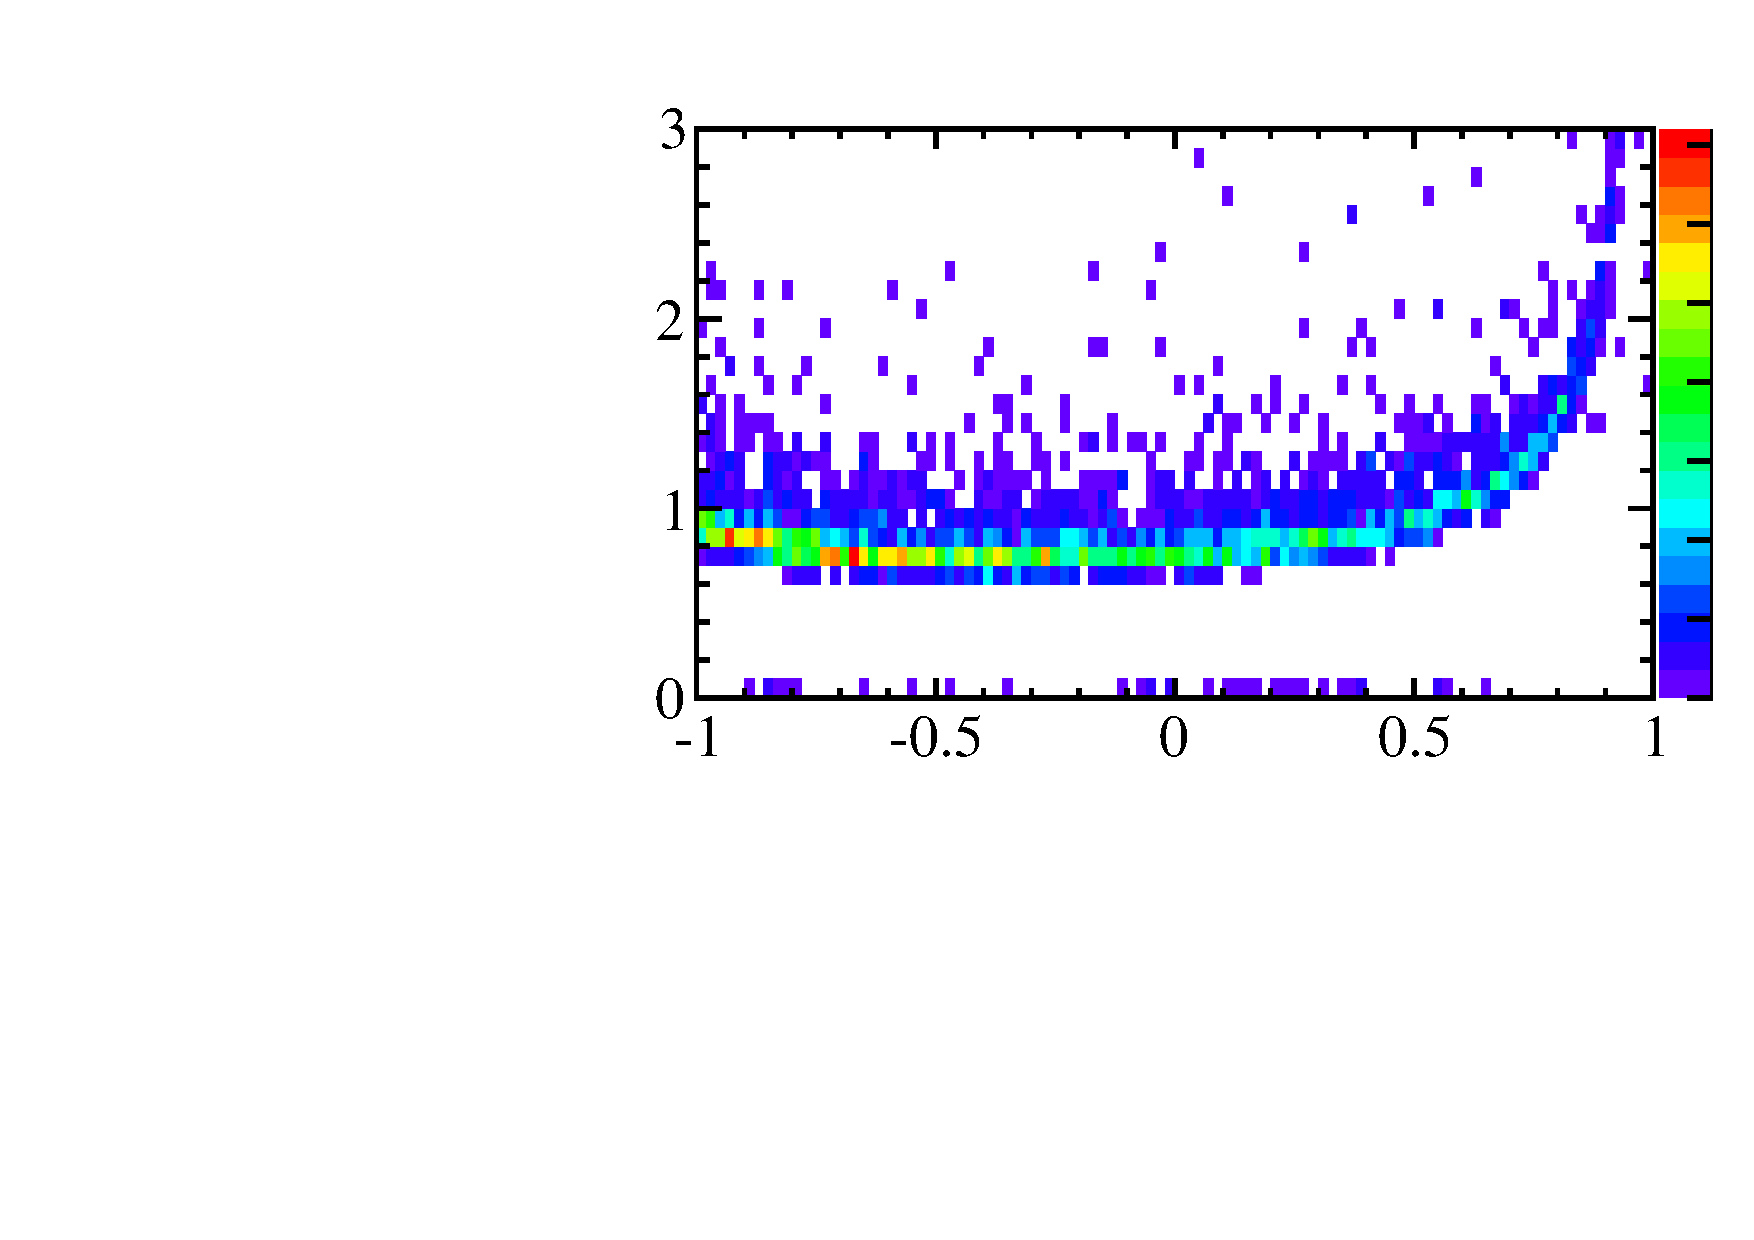
\includegraphics[width=0.48\columnwidth]{chapter5/figs/sys/validation_weight_ctk_hadronpcut.pdf}}
%\subfigure[]{
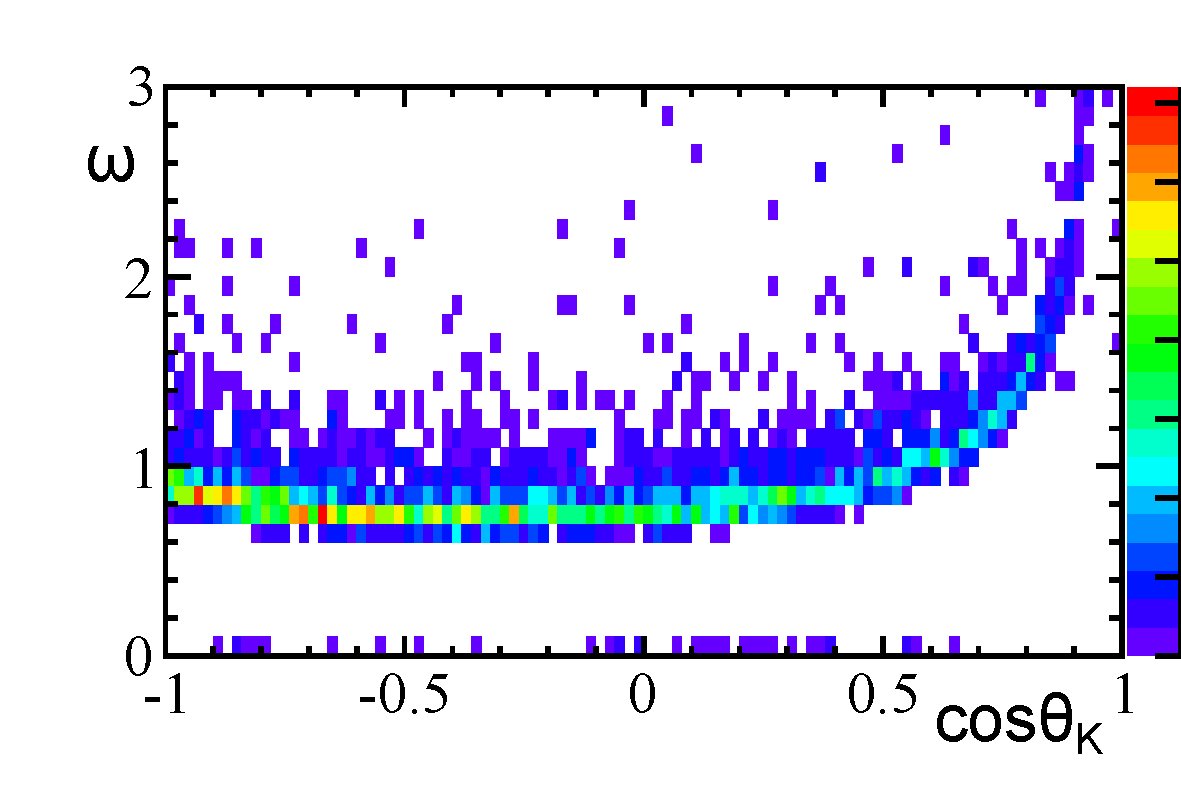
\includegraphics[width=0.48\columnwidth]{chapter5/figs/sys/validation_weight_ctk_hadronpcut_new.pdf}
%}
\caption[  The effect of the removal of all hadrons of $p<3\gevc$ from the phase space simulation used in the acceptance correction.  ]
{ The effect of the removal of all hadrons of $p<3\gevc$ from the phase space simulation used in the acceptance correction. 
%The effect on a re-weighted phase space sample is shown in (a) where 
It is possible to see the artificially higher weights at high values of \ctk. 
%The effect on the weight values on the data sample is shown in (b). 
~\label{fig:kstmm:sys:hadronp} }
\end{figure}
%The estimate of the systematic uncertainty from this cut is not propagated to the final uncertainty because it is not a realistic .

\subsubsection{Mass Model}

There is a systematic effect from using the same mass model for the multiple different \qsq bins.
The widths of the two Crystal Ball functions used for the signal mass model are checked using 
corrected simulated \BdToKstmm data. The width is found to vary within errors to $\pm5\%$ and
both widths in the signal mass model are varied by this amount to compensate for this.

The systematic uncertainty on the parametrisation of the angular background is estimated by using a 
constant background as opposed to a $2^{\text{nd}}$ order Chebychev polynomial.
This has no significant impact on the values of the angular observables.

\subsubsection{Event Selection}

The two sources of possible systematic uncertainty from the event selection are from the 
consideration of peaking backgrounds and from the treatment of multiple candidates.
Peaking background decays such as \Bs\to\Kstarz\mumu and \Bs\to\varphi\mumu are difficult to account
for in the angular fit because the angular distribution of the decay products is not well known.
A conservative estimate of the contribution from these decays is assumed by assigning a
5\% systematic to the events that have $\AFB=\pm1$, $\FL=0,1$.
This method gives a total estimate of the systematic uncertainty from peaking backgrounds of approximately 2\%.

The treatment of multiple candidates is systematically accounted for by removing all events with multiple 
candidates.
The fraction of events with multiple candidates is between 1-2\% and consists mainly of \ktopi swapped candidates.
This has no impact on the final values for the angular observables.

\subsubsection{Tables of systematic uncertainties}




\section{Results}
\label{sec:kstmm:res}

The results for the angular analysis of \BdToKstmm for .38\invfb and 1.0\invfb of data collected at \lhcb are presented below.
A measurement of the differential branching fraction of \BdToKstmm was obtained by fitting
 the invariant mass distribution of selected candidates in each \qsq bin and normalising to \BdToJpsiKstar. 

\subsection{Angular analysis of 0.38\invfb of data}

The invariant mass distribution of the selected \BdToKstmm candidates in the data is shown in Fig.~\ref{fig:res1massfit}.
\begin{figure}[tbp]
\centering
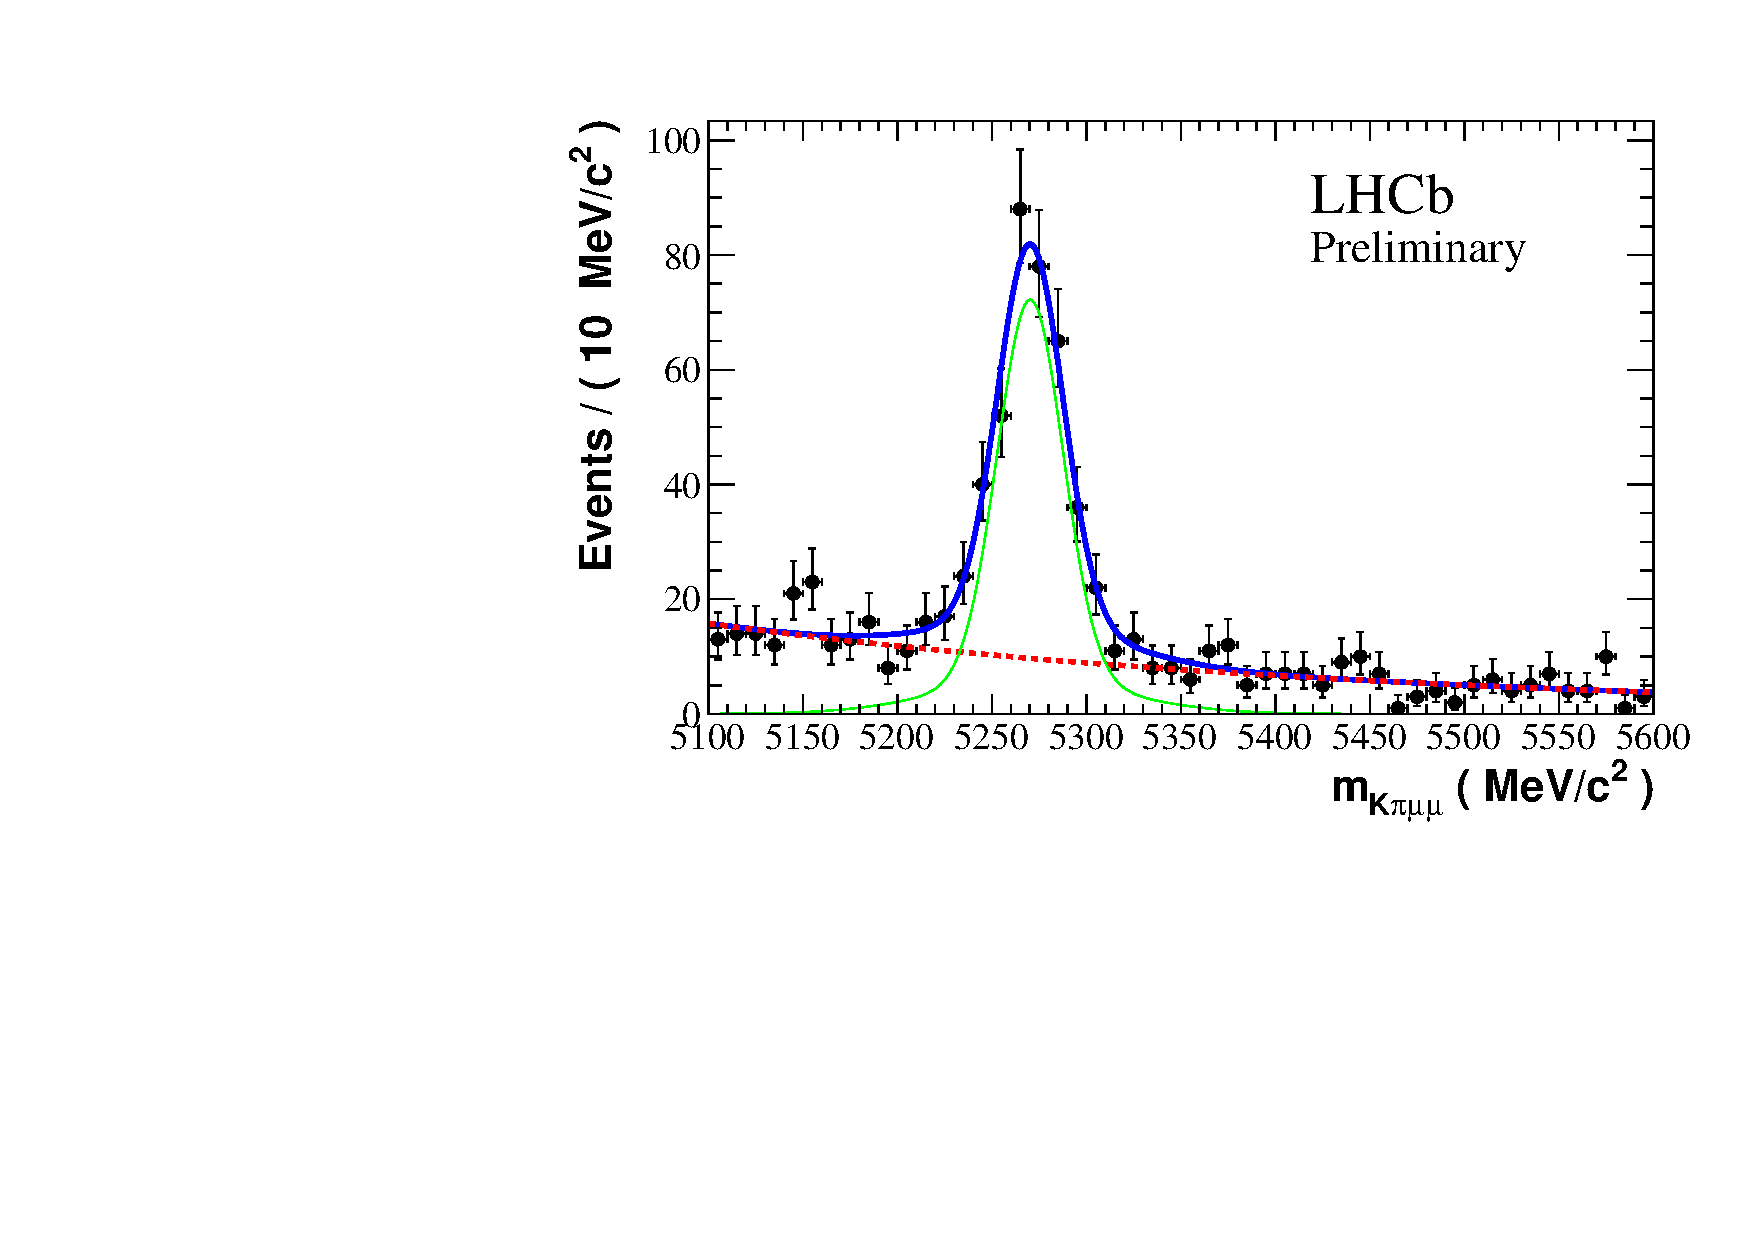
\includegraphics[scale=0.33]{chapter5/figs/results1/mass_fit_full.pdf}
\caption[The fit to the \mkpimm invariant mass distribution of selected \BdToKstmm candidates from 0.37\invfb.]
{The fit to the \mkpimm invariant mass distribution of selected \BdToKstmm candidates from 0.37\invfb.
 The fit to the mass distribution gives an estimate of $337\pm21$ signal events. ~\label{fig:res1massfit}}
\end{figure}
The fit gives an estimate of $337\pm21$ signal events with a background of $97\pm6$ events.
The measured values of \AFB, \FL and the differential branching fraction of \BdToKstmm are shown in Fig.~\ref{fig:kstmm:res1}.
%along with a theoretical prediction from Ref.~\cite{Bobeth:2011gi}. 
\begin{figure}[tbp]
\centering
\subfigure[]{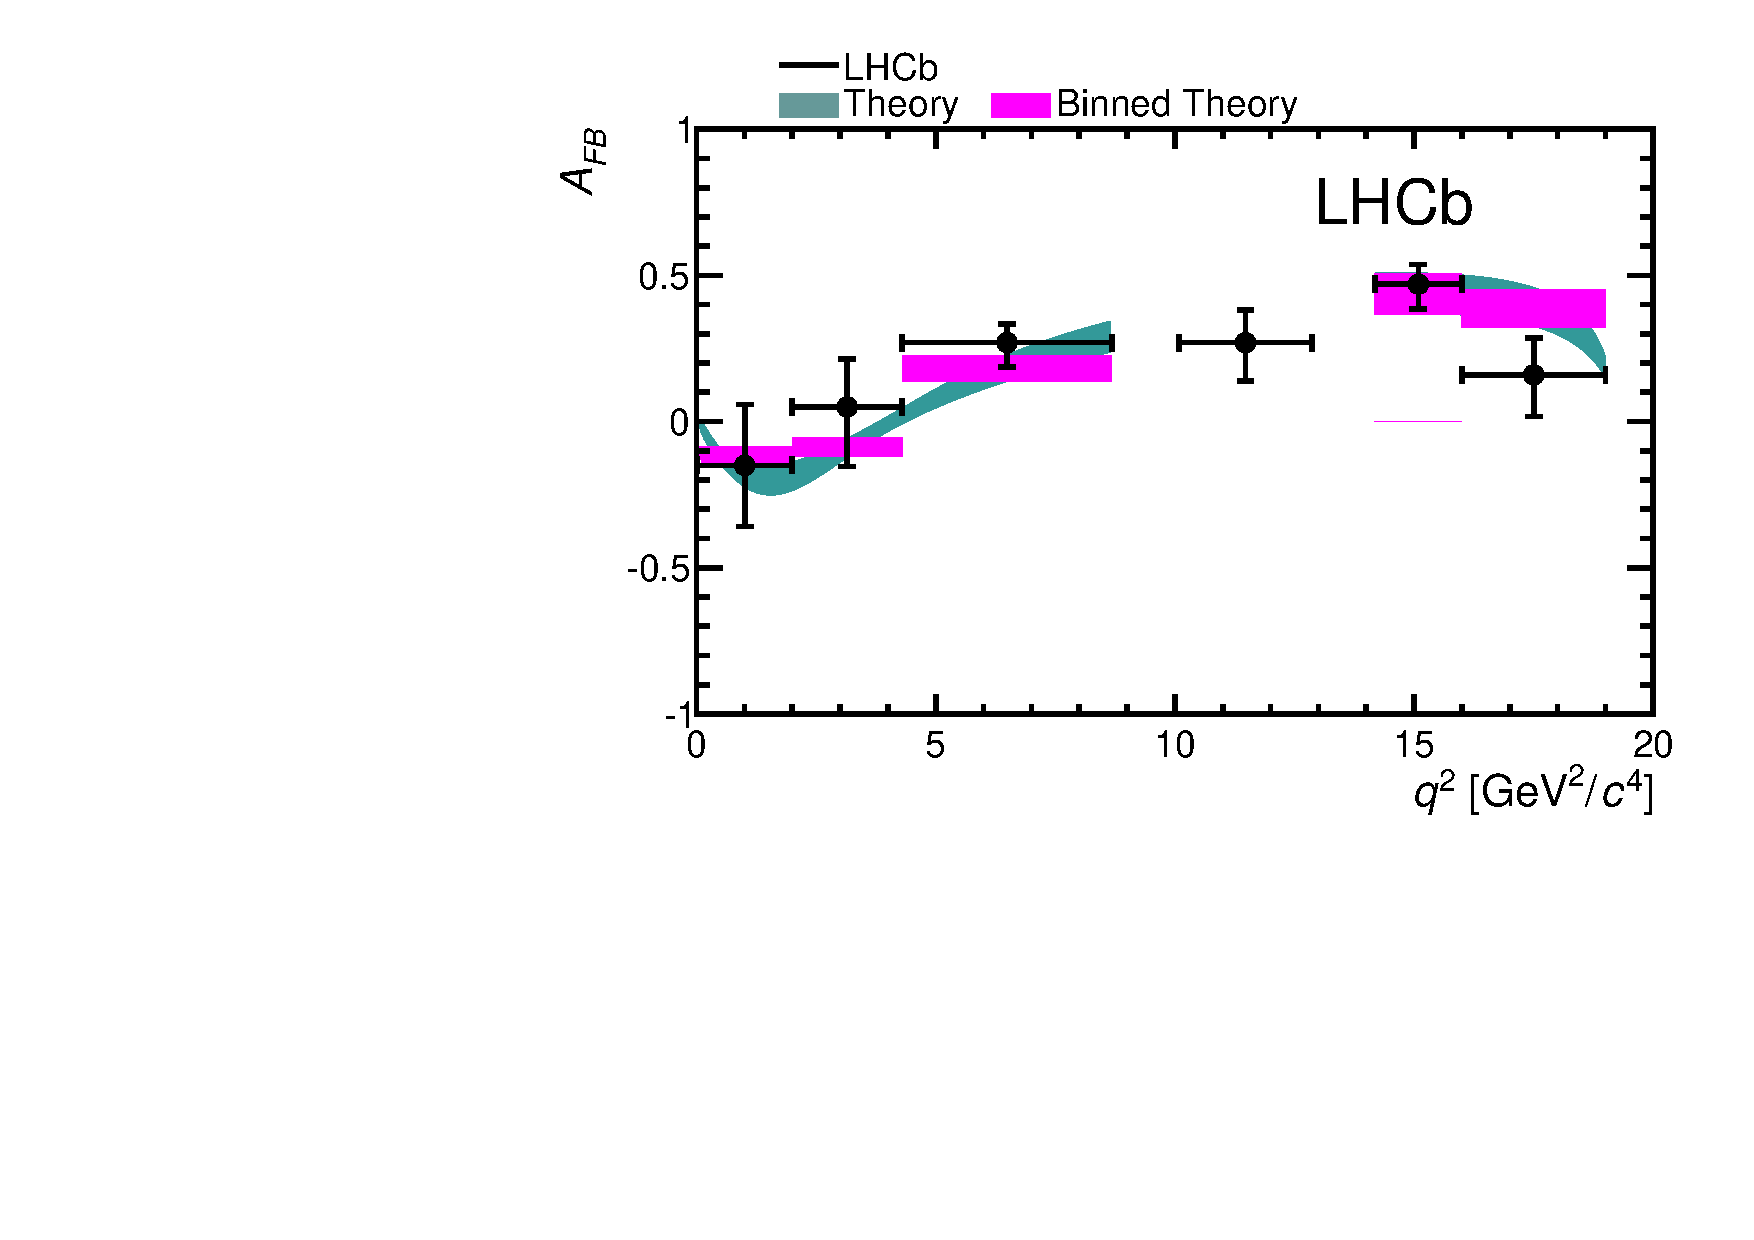
\includegraphics[scale=0.33]{chapter5/figs/results1/plot_AFB1.pdf}}
\subfigure[]{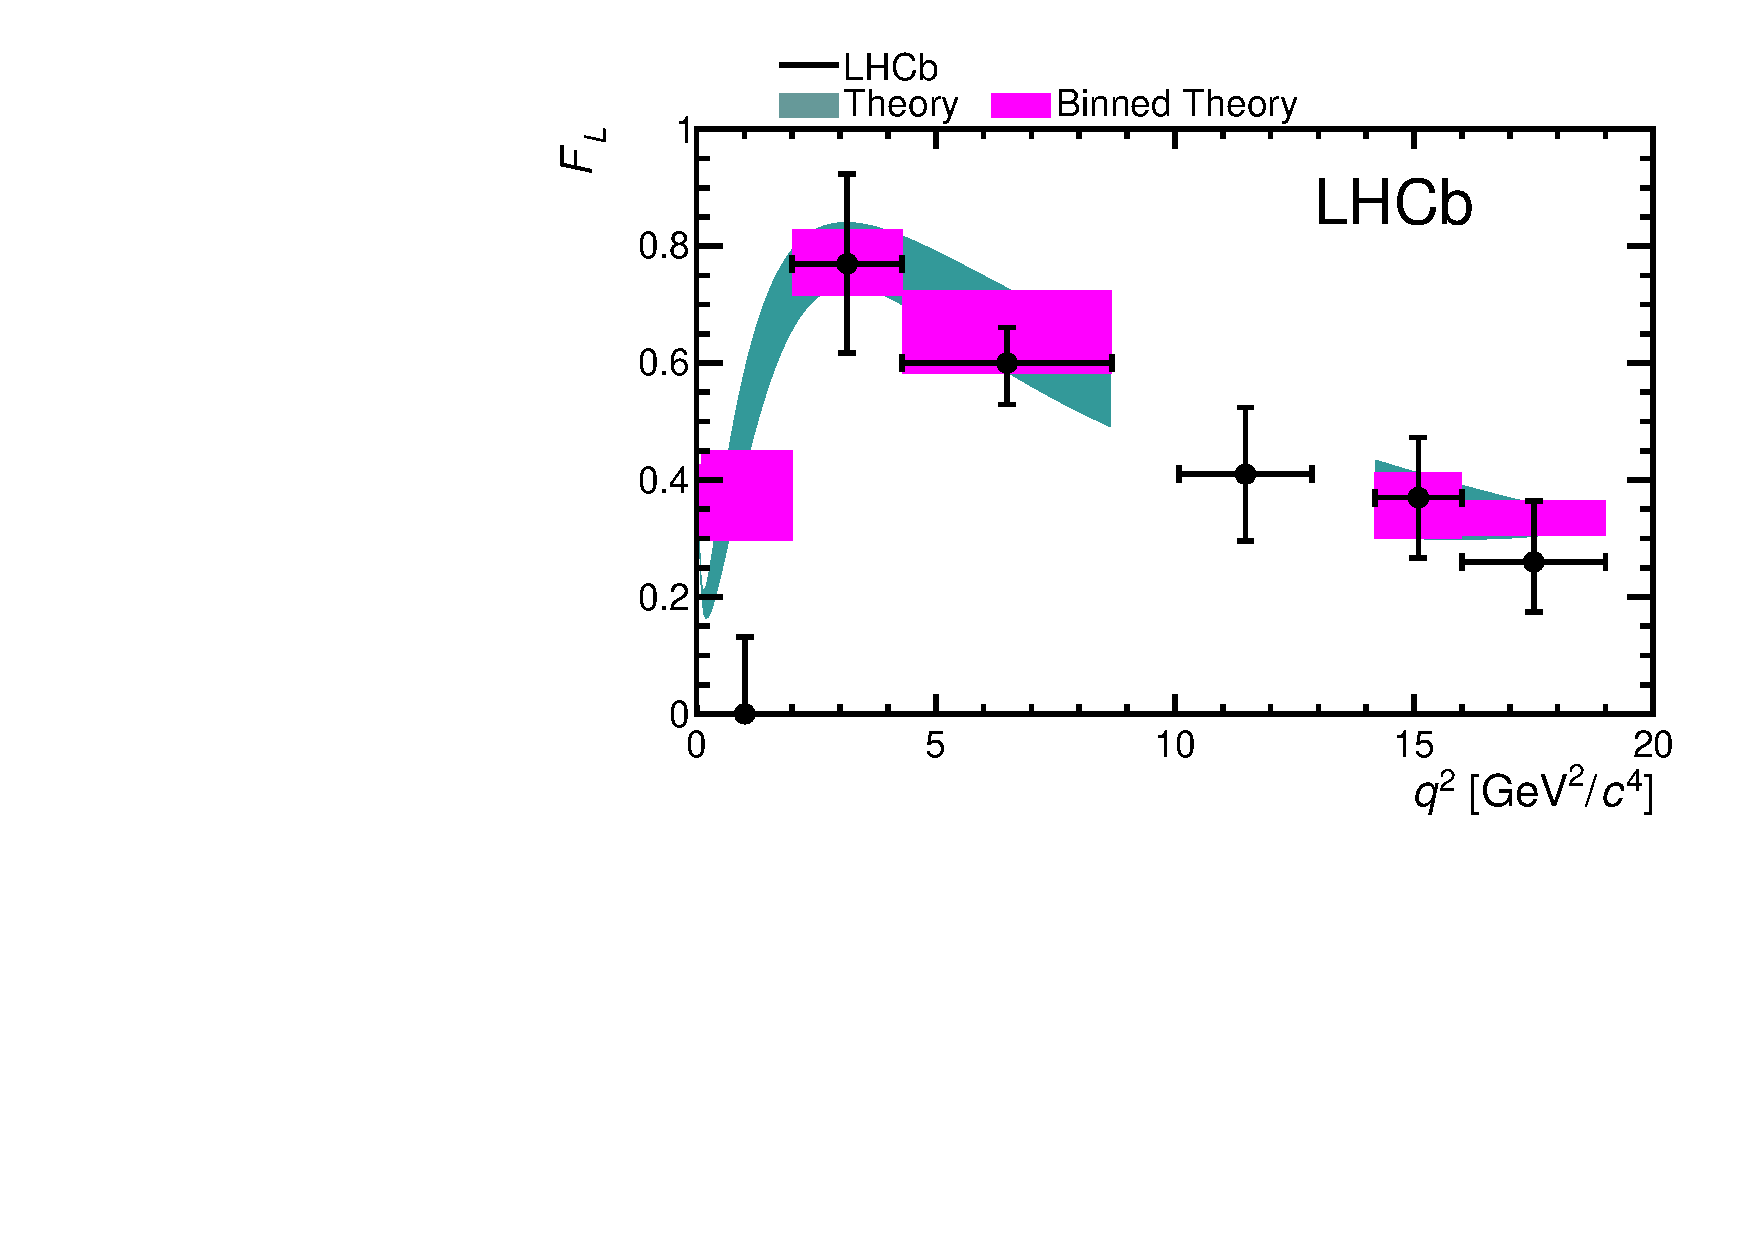
\includegraphics[scale=0.33]{chapter5/figs/results1/plot_FL1.pdf}}
\subfigure[]{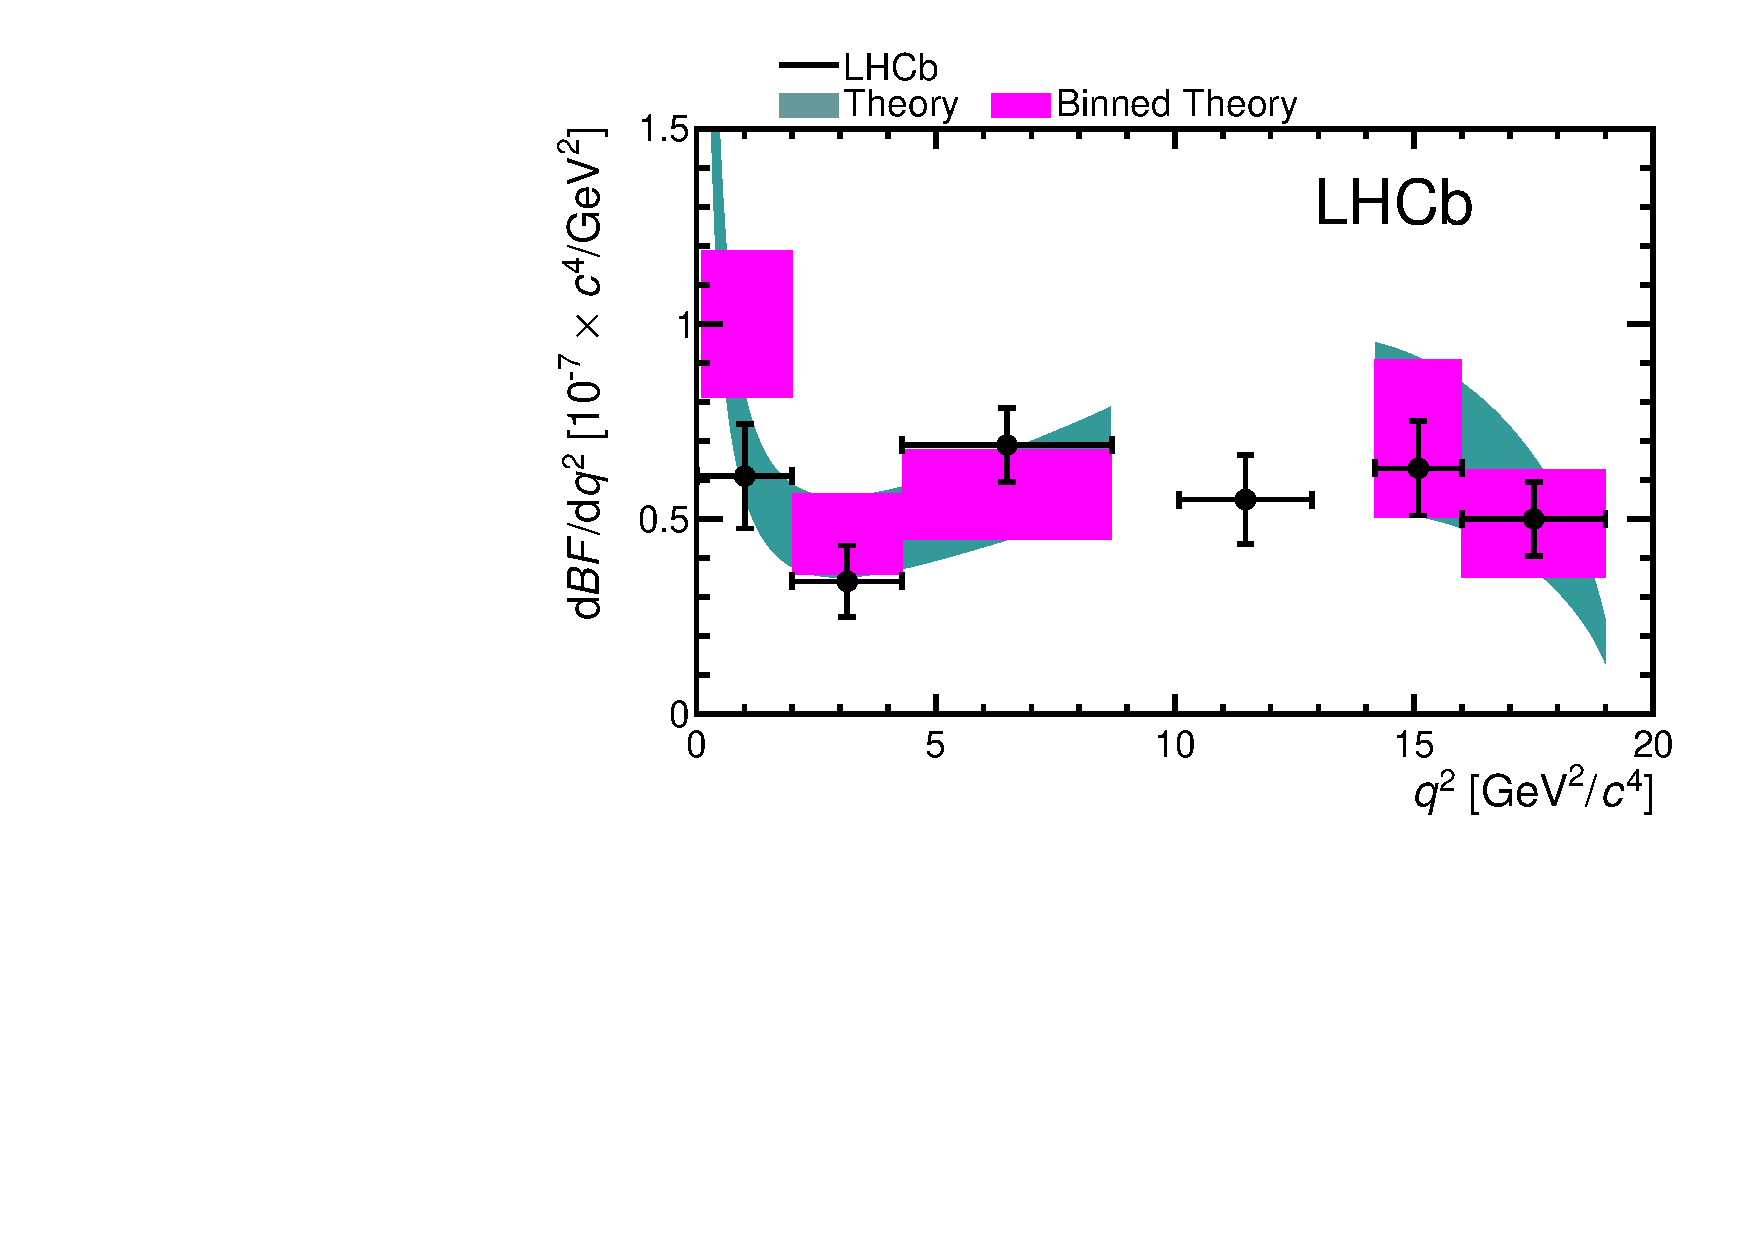
\includegraphics[scale=0.33]{chapter5/figs/results1/plot_Width1.pdf}}
\caption[  The final results from the angular analysis of \BdToKstmm at \lhcb using 0.38\invpb of data collected in 2011 at 7 \tev. ]
{The final results from the angular analysis of \BdToKstmm at \lhcb using 0.38\invpb of data collected in 2011 at 7 \tev. 
Values for \AFB, \FL and the differential branching fraction are extracted in the six different bins of \qsq.
The Standard Model prediction is from~\cite{Bobeth:2011gi}
~\label{fig:kstmm:res1}}
\end{figure}
The central values for the angular observables along with the statistical and systematic errors are given in Table~\ref{table:kstmm:res1}.
\begin{table}[tbp]
\centering
\caption[ The central values and statistical plus systematic uncertainties
 for $A_{FB}$, $F_{L}$ and  $d{\BF}/dq^{2}$ for the 0.38\invfb angular analysis.   ]
{The central values and statistical plus systematic uncertainties
 for $A_{FB}$, $F_{L}$ and  $d{\BF}/dq^{2}$ for the 0.38\invfb angular analysis. 
The first, asymmetric, set of errors is given by the Bayesian error estimate, 
with a prior that the points sit within the physical region. 
The second error is the systematic error on $A_{FB}$, $F_{L}$ and the branching fraction.
\label{table:kstmm:res1}
}
\vspace{5mm}
\begin{tabular}{|c|c|c|c|}
\hline
$\qsq (\gevgevcccc) $ & \AFB & \FL & $d\BF/d\qsq$ ($\times10^{-7} \gev^{-2} c^{4}$)  \\  \hline
$0.10 < q^{2} < 2.00$ & $-0.15^{+0.20}_{-0.20}\pm 0.06$ & $0.00^{+0.13}_{-0.00}\pm 0.02$ & $0.61 \pm 0.12\pm 0.06$ \\
$2.00 < q^{2} < 4.30$ & $+0.05^{+0.16}_{-0.20}\pm 0.04$ & $0.77^{+0.15}_{-0.15} \pm 0.03$ & $0.34 \pm 0.09\pm 0.02$ \\ 
$4.30 < q^{2} < 8.68$ & $+0.27^{+0.06}_{-0.08}\pm 0.02$ & $0.60^{+0.06}_{-0.07} \pm 0.01$ & $0.69 \pm 0.08\pm 0.05$ \\ 
$10.09 < q^{2} < 12.86$ & $+0.27^{+0.11}_{-0.13}\pm 0.02 $ & $0.41^{+0.11}_{-0.11} \pm 0.03$ & $0.55 \pm 0.09\pm 0.07$ \\ 
$14.18 < q^{2} < 16.00$ &  $+0.47^{+0.06}_{-0.08}\pm 0.03$ & $0.37^{+0.09}_{-0.09}\pm 0.05$ & $0.63 \pm 0.11\pm 0.05$ \\ 
$16.00 < q^{2} < 19.00$ & $+0.16^{+0.11}_{-0.13}\pm 0.06$ & $0.26^{+0.10}_{-0.08}\pm 0.03$ & $0.50 \pm 0.08\pm 0.05$ \\
$1.00 < q^{2} < 6.00$ & $-0.06^{+0.13}_{-0.14}\pm 0.04$ & $0.55^{+0.10}_{-0.10}\pm 0.03$ & $0.42 \pm 0.06\pm 0.03$ \\
\hline
\end{tabular}
\end{table}
All of the values for the angular observables lie within the physical limits of \AFB and \FL (Section~\ref{sec:kstmm:obs}) except for the values for the
 $14.18<\qsq<16\gev^2$ bin.
The statistical errors for the physically valid \AFB and \FL values are given by the Bayesian error estimate with a prior that the points sit within the physical region. 
To extract a physical value for the  $14.18<\qsq<16\gev^2$ bin, the lowest value of the likelihood was taken and the errors obtained by integrating 
the likelihood to reach one $\sigma$ coverage.
These were the most precise measurements of the angular observables at the time of publication.


\subsection{Analysis of 1.0\invfb of data}

%The results of the angular analysis of \BdToKstmm at \lhcb using 1.0\invfb of data collected in 2011 are presented below.
The invariant mass distribution of selected \BdToKstmm candidates is shown in Fig.~\ref{fig:res2massfit}  
and there are an estimated $900\pm34$ signal candidates in 1.0\invfb of data. 
\begin{figure}[tbp]
\centering
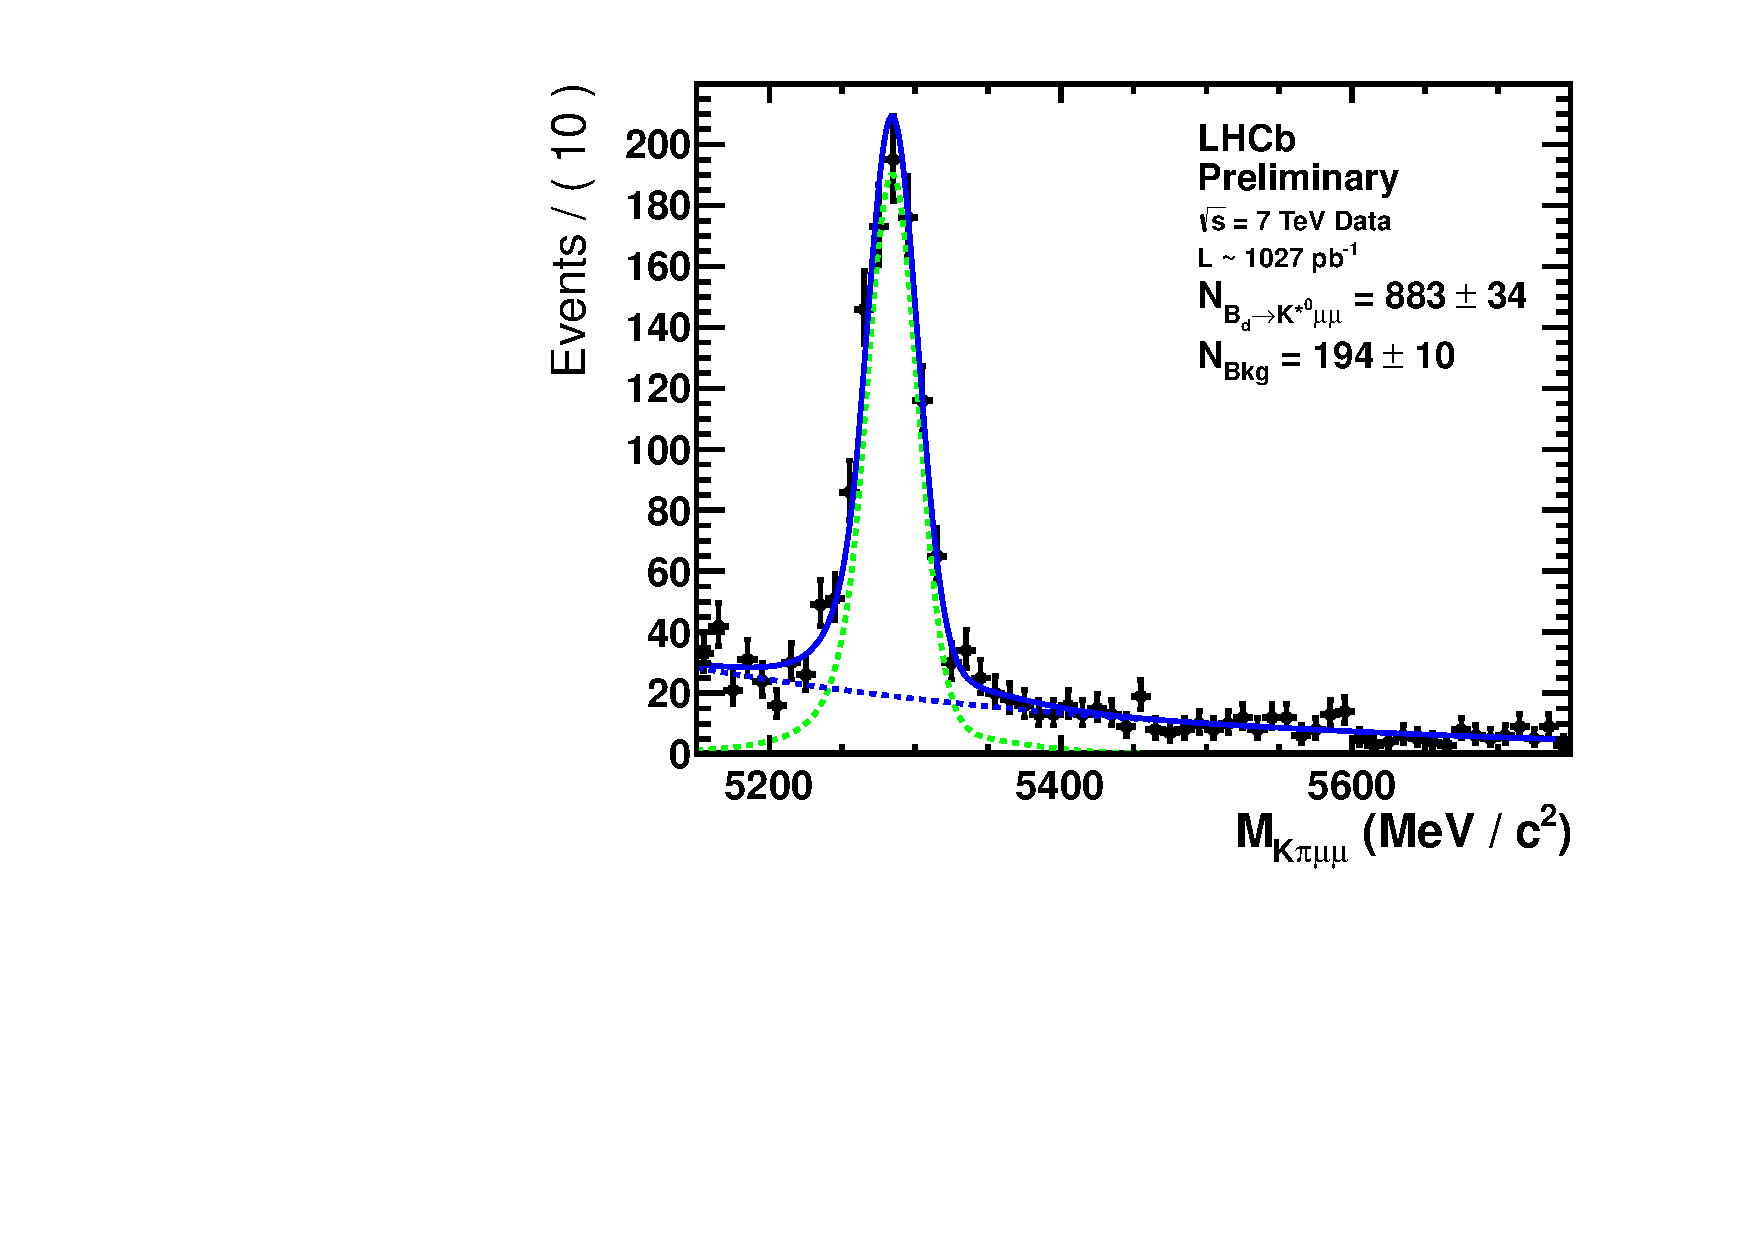
\includegraphics[scale=0.33]{chapter5/figs/results2/KstarMuMuFit_q2low_0_1_q2high_19.pdf}
\caption[ The fit to invariant mass distribution of selected \BdToKstmm candidates from 1.0\invfb of data.  ]
{The fit to invariant mass distribution of selected \BdToKstmm candidates from 1.0\invfb of data.
The fit gives and estimate of $900\pm34$ candidates.~\label{fig:res2massfit}}
\end{figure}
The results for seven angular observables are presented in Table~\ref{table:kstmm:res2}.
The values for the differential branching fraction are presented in Table~\ref{table:kstmm:dbr2}.
\begin{table}[tbp]
\centering
\caption[Fraction of longitudinal polarisation of the \Kstarz, \FL, 
dimuon system forward backward asymmetry, \AFB, and the angular observables 
\OS3, \OS9 and \OA9 from the \BdToKstmm decay in six bins of \qsq.   ]
{Fraction of longitudinal polarisation of the \Kstarz, \FL, 
dimuon system forward backward asymmetry, \AFB, and the angular observables 
\OS3, \OS9 and \OA9 from the \BdToKstmm decay in six bins of \qsq. 
The lower table includes the transverse observables \ATRe and \AT2 
that are thought to have reduced form factor uncertainties. Results are also presented
 in the $1 < \qsq < 6\gevgevcccc$ range where theoretical uncertainties are 
best controlled.  \label{table:kstmm:res2}}
\begin{tabular}{|c|c|c|c|c|} 
\hline
\qsq $(\gevgevcccc)$ & \FL & \AFB & \OS3 & \OS9 \\
\hline
$0.10 - 2.00$ & $0.36\,^{+0.11}_{-0.10}\,^{+0.05}_{-0.03}$ & $-0.02\,^{+0.13}_{-0.12}\,^{+0.03}_{-0.00}$ & $-0.05\,^{+0.09}_{-0.10}\,^{+0.01}_{-0.01}$ & $\phantom{-}0.06\,^{+0.10}_{-0.10}\,^{+0.01}_{-0.00}$ \\
$2.00 - 4.30$ & $0.74\,^{+0.01}_{-0.12}\,^{+0.02}_{-0.02}$ & $-0.20\,^{+0.08}_{-0.08}\,^{+0.02}_{-0.01}$ & $-0.04\,^{+0.09}_{-0.08}\,^{+0.01}_{-0.01}$ & $-0.03\,^{+0.11}_{-0.04}\,^{+0.01}_{-0.01}$ \\
$4.30 - 8.68$ & $0.55\,^{+0.08}_{-0.07}\,^{+0.03}_{-0.03}$ & $\phantom{-}0.16\,^{+0.05}_{-0.06}\,^{+0.01}_{-0.02}$ & $\phantom{-}0.07\,^{+0.07}_{-0.08}\,^{+0.01}_{-0.01}$ & $\phantom{-}0.01\,^{+0.07}_{-0.08}\,^{+0.01}_{-0.00}$ \\
$10.09 - 12.86$ & $0.48\,^{+0.09}_{-0.07}\,^{+0.02}_{-0.04}$ & $\phantom{-}0.28\,^{+0.07}_{-0.06}\,^{+0.02}_{-0.02}$  & $-0.16\,^{+0.11}_{-0.08}\,^{+0.01}_{-0.01}$ & $-0.02\,^{+0.12}_{-0.11}\,^{+0.01}_{-0.01}$\\
$14.18 - 16.00$ & $0.33\,^{+0.08}_{-0.09}\,^{+0.02}_{-0.03}$ & $\phantom{-}0.51\,^{+0.08}_{-0.05}\,^{+0.02}_{-0.02}$ & $\phantom{-}0.03\,^{+0.09}_{-0.11}\,^{+0.02}_{-0.01}$ &  $\phantom{-}0.00\,^{+0.10}_{-0.09}\,^{+0.01}_{-0.01}$\\
$16.00 - 19.00$ & $0.38\,^{+0.10}_{-0.08}\,^{+0.03}_{-0.03}$ & $\phantom{-}0.30\,^{+0.08}_{-0.08}\,^{+0.01}_{-0.02}$ & $-0.22\,^{+0.11}_{-0.09}\,^{+0.02}_{-0.01}$ & $\phantom{-}0.06\,^{+0.11}_{-0.11}\,^{+0.01}_{-0.02}$ \\
\hline
$1.00 - 6.00$ & $0.65\,^{+0.08}_{-0.07}\,^{+0.03}_{-0.03}$ & $-0.15\,^{+0.07}_{-0.07}\,^{+0.02}_{-0.01}$ & $-0.03\,^{+0.08}_{-0.08}\,^{+0.01}_{-0.00}$ & $-0.05\,^{+0.08}_{-0.08}\,^{+0.01}_{-0.01}$ \\
\hline
\end{tabular}
\vspace{.5cm}\\
\begin{tabular}{|c|c|c|c|}
\hline
\qsq $(\gevgevcccc)$ & \OA9 & \AT2 & \ATRe \\
\hline
$0.10 - 2.00$ & $\phantom{-}0.12\,_{-0.09}^{+0.10}\,^{+0.01}_{-0.01}$ & $-0.16\,_{-0.31}^{+0.30}\,^{+0.03}_{-0.03}$ & $-0.04\,_{-0.24}^{+0.25}\,^{+0.03}_{-0.01}$ \\
$2.00 - 4.30$ & $\phantom{-}0.07\,_{-0.09}^{+0.12}\,^{+0.00}_{-0.01}$ & $-0.32\,_{-0.49}^{+0.65}\,^{+0.05}_{-0.04}$ & $-1.00\,_{-0.00}^{+0.15}\,^{+0.05}_{-0.01}$ \\
$4.30 - 8.68$ &	$-0.14\,_{-0.06}^{+0.07}\,^{+0.02}_{-0.01}$  & $\phantom{-}0.33\,_{-0.31}^{+0.30}\,^{+0.01}_{-0.05}$ & $\phantom{-}0.51\,_{-0.14}^{+0.15}\,^{+0.00}_{-0.05}$ \\
$10.09 - 12.86$ & $\phantom{-}0.00\,_{-0.11}^{+0.12}\,^{+0.01}_{-0.01}$ &	$-0.60\,_{-0.18}^{+0.41}\,^{+0.06}_{-0.02}$ & $\phantom{-}0.72\,_{-0.15}^{+0.14}\,^{+0.02}_{-0.03}$ \\
$14.18 - 16.00$ & $-0.07\,_{-0.08}^{+0.11}\,^{+0.02}_{-0.00}$ & $\phantom{-}0.07\,_{-0.28}^{+0.26}\,^{+0.00}_{-0.04}$ & $\phantom{-}1.00\,_{-0.05}^{+0.00}\,^{+0.01}_{-0.02}$ \\ 
$16.00 - 19.00$ & $\phantom{-}0.00\,_{-0.10}^{+0.11}\,^{+0.01}_{-0.01}$ & $-0.71\,_{-0.25}^{+0.34}\,^{+0.07}_{-0.04}$ & $\phantom{-}0.64\,_{-0.14}^{+0.14}\,^{+0.01}_{-0.03}$ \\ 
\hline
$1.00 - 6.00$ & $\phantom{-}0.02\,^{+0.08}_{-0.08}\,^{+0.01}_{-0.00}$ & $\phantom{-}0.15\,_{-0.42}^{+0.39}\,^{+0.04}_{-0.02}$ & $-0.57\,_{-0.22}^{+0.25}\,^{+0.03}_{-0.06}$\\ 
\hline
\end{tabular} 
\end{table}
\begin{table}
\centering
\caption[ Signal yield ($N_{\text{sig}}$) and differential branching fraction
 ($\deriv\BF/\deriv\qsq$) of the \decay{\Bz}{\Kstarz\mumu} decay.   ]
{Signal yield ($N_{\text{sig}}$) and differential branching fraction
 ($\deriv\BF/\deriv\qsq$) of the \decay{\Bz}{\Kstarz\mumu} decay in the six \qsq bins used in this analysis.
 Results are also presented in the $1 < \qsq < 6\gev^{2}/c^{4}$ range where theoretical uncertainties are best controlled. 
The final uncertainty on $\deriv\BF/\deriv\qsq$ comes from an estimate of the pollution from 
 \decay{\Bz}{\Kp\pim\mumu} in the $792 < m_{\Kp\pim} < 992\mevcc$ mass window. 
 \label{table:kstmm:dbr2}}
\begin{tabular}{|c|c|c|} 
\hline
\qsq $(\gev^{2}/c^{4})$ & $N_{\text{sig}}$ & $\deriv\BF/\deriv\qsq$ $(10^{-7} \gev^{-2} c^{4})$ \\
\hline
$0.10 - 2.00$ & $140 \pm 13$ & $0.61\pm 0.08 \pm 0.05 \,^{+0.00}_{-0.05}$ \\
$2.00 - 4.30$ & $\phantom{0}73 \pm 11$ & $0.30\pm 0.05 \pm 0.03 \,^{+0.00}_{-0.02}$ \\
$4.30 - 8.68$ & $271 \pm 19$ & $0.50\pm 0.05 \pm 0.04 \,^{+0.00}_{-0.04}$ \\
$10.09 - 12.86$ & $168 \pm 15$ & $0.43\pm 0.05 \pm 0.04 \,^{+0.00}_{-0.03}$ \\
$14.18 - 16.00$ & $115 \pm 12$ & $0.57\pm 0.07 \pm 0.04 \,^{+0.00}_{-0.05}$ \\
$16.00 - 19.00$ & $116 \pm 13$ & $0.42\pm 0.05 \pm 0.04 \,^{+0.00}_{-0.03}$ \\
\hline
$1.00 - 6.00$ & $197 \pm 17$ & $0.35\pm 0.04 \pm 0.04 \,^{+0.00}_{-0.03}$ \\
\hline
\end{tabular}
\end{table}
The results are also shown in Fig.~\ref{fig:kstmm:res2:norm}, Fig.~\ref{fig:kstmm:res2:reparam},
and Fig.~\ref{fig:kstmm:res2:a9dbr} along with the theoretical prediction from~\cite{Bobeth:2011gi} where available.
\begin{figure}[tbp]
\centering
\subfigure[]{\includegraphics[scale=0.31]{chapter5/figs/paper2/cAFB.pdf}}
\subfigure[]{\includegraphics[scale=0.31]{chapter5/figs/paper2/cFL.pdf}}
\subfigure[]{\includegraphics[scale=0.31]{chapter5/figs/paper2/cS3.pdf}}
\subfigure[]{\includegraphics[scale=0.31]{chapter5/figs/paper2/cS9.pdf}}
\caption[ The final results from the angular analysis of \BdToKstmm at \lhcb using 1.0\invfb of data collected in 2011 at 7 \tev.   ]
{The final results from the angular analysis of \BdToKstmm at \lhcb using 1.0\invfb of data collected in 2011 at 7 \tev. 
Values for the original observables are extracted in the six different bins of \qsq.
The Standard Model prediction is from~\cite{Bobeth:2011gi}.
~\label{fig:kstmm:res2:norm}}
\end{figure}
\begin{figure}[tbp]
\centering
\subfigure[]{\includegraphics[scale=0.31]{chapter5/figs/paper2/cATRE.pdf}}
%\subfigure[]{\includegraphics[scale=0.31]{chapter5/figs/results2/plot_ATI.pdf}}
\subfigure[]{\includegraphics[scale=0.31]{chapter5/figs/paper2/cAT2.pdf}}
\subfigure[]{\includegraphics[scale=0.31]{chapter5/figs/paper2/cA9.pdf}}
%\subfigure[]{\includegraphics[scale=0.31]{chapter5/figs/results2/plot_Width.pdf}}
\caption[ The final results from the angular analysis of \BdToKstmm at \lhcb using 1.0\invfb of data collected in 2011 at 7 \tev.   ]
{The final results from the angular analysis of \BdToKstmm at \lhcb using 1.0\invfb of data collected in 2011 at 7 \tev. 
Values for the the reparameterised observables and the CP asymmetric observable \OA9 are extracted in the six different bins of \qsq.
The Standard Model prediction is from~\cite{Bobeth:2011gi}.
~\label{fig:kstmm:res2:reparam}}
\end{figure}
\begin{figure}[tbp]
\centering
\subfigure[]{\includegraphics[scale=0.31]{chapter5/figs/paper2/cWidth.pdf}}
\caption[  The final results from the angular analysis of \BdToKstmm at \lhcb using 1.0\invfb of data collected in 2011 at 7 \tev.  ]
{The final results from the angular analysis of \BdToKstmm at \lhcb using 1.0\invfb of data collected in 2011 at 7 \tev. 
The differential branching fraction is extracted in the six different bins of \qsq.
The Standard Model prediction is from~\cite{Bobeth:2011gi}.
~\label{fig:kstmm:res2:a9dbr}}
\end{figure}













%\section{Interpretation}

The first angular analysis of \BdToKstmm has been interpreted both in context of placing constraints of the values of
the Wilson coefficients \C7, \C9 and \C10 ~\cite{Bobeth:2011nj}.
The constraints placed by measurements of electroweak penguin decays on the absolute 
magnitude of \C9 and \C10 are shown in Fig~\ref{fig:c9vsc10}.
\begin{figure}[tb]
\centering
\includegraphics[width=0.48\columnwidth]{chapter5/figs/theo/fig-constraints-c9-c10-all-all-all-contour.pdf}
\caption{ Constraints on the $|\C9 |$ v.s. $|\C10 |$ using the measurements of electroweak penguin decays
 available towards the end of 2011. Taken from Ref.~\cite{Bobeth:2011nj}.~\label{fig:c9vsc10} }
\end{figure}
A second interpretation of \BdToKstmm in the context of similar heavy flavour decays has also placed constraints on 
the values of the Wilson coefficients using the results from the first and second angular analyses respectively
~\cite{Altmannshofer:2011gn,Altmannshofer:2012az}.
It is possible to see that the measurements presented in this chapter provide some of the most stringent constraints on
 the values of the Wilson coefficients from \bquark\to\squark decays.




\section{Conclusions}

The angular analysis of \BdToKstmm  at \lhcb was performed on 
both 0.38\invfb and 1.0\invfb of data taken in 2011. 

Clean samples of \BdToKstmm candidates were selected using both a cut-based selection and a multi-variate algorithm. 
There were around 340 candidates in 0.38\invfb and 900 candidates in 1.0\invfb of data.
The first dataset is comparable to previous results from the \babar, \belle and \cdf 
and the second dataset is the largest sample of \BdToKstmm candidates at one experiment to date.

The candidates were corrected for the acceptance effect introduced by the reconstruction and selection by applying a weight to each event.
The first analysis used a $k$-nearest-neighbour method to calculate the efficiency to selected simulated events at a point in \ctl and \ctk.
This was an accurate calculation but the prevision and accuracy was limited by the number of simulated candidates in the regions of phase space with low efficiency.
The second analysis calculated the efficiency from a function fitted to each of the \ctl, \ctk and \varphi distributions independently.
This limitation of this method is that it assumes that the efficiency factorises into each dimension, which introduces additional sources of systematic uncertainty.
The method of weighting each of the \BdToKstmm candidate for their acceptance was chosen over the alternative method,
 of combining the signal model and a function for the efficiency, in order to minimise the number of free parameters in the final model. 	
This allowed measurement of the angular observables using the multi-dimensional angular distribution which fully incorporated the correlations between the angular observables.

The acceptance effect and the data-simulation corrections were the dominant sources of systematic uncertainty for both analyses. 
This is because the events with lowest efficiency, at extreme \ctl and high \ctk, have a large effect on the central value of \AFB and \FL.
This can be improved by a better understanding of the simulation and the efficiency to select \BdToKstmm candidates
 but the understanding of the efficiency in this region of phase space is a limitation on the accuracy of the measurement.

The first angular analysis obtained the worlds most precise measurements of the observables \AFB and \FL as well as measuring the differential branching fraction.
The second angular analysis improved the measurements of \AFB and \FL 
as well as measuring several new angular observables for the first time.
The measurements of \AFB and \FL from \lhcb along with the measurements from \babar, \belle and \cdf are shown in Figure~\ref{fig:res:comboexp}.
\begin{figure}[tbp]
\centering
\subfigure[]{\includegraphics[width=0.48\columnwidth]{chapter5/figs/plot_FLExp.pdf}}
\subfigure[]{\includegraphics[width=0.48\columnwidth]{chapter5/figs/plot_AFBExp.pdf}}
\caption{The measurements of the angular observables \FL and \AFB from \lhcb, \babar~\cite{Aubert:2007hz,Aubert:2008ju}, 
\belle~\cite{PhysRevLett.103.171801}  and \cdf~\cite{Aaltonen:2011cn,Aaltonen:2011ja} along with the theoretical prediction from Ref.~\cite{Bobeth:2011gi}. 
It is possible to see that the \lhcb results are the most precise and are compatible with the SM prediction.~\label{fig:res:comboexp}}
\end{figure}

The combination of these results, along with other radiative,
semi-leptonic and purely leptonic decays has enabled stringent limits to be set on the 
values for the Wilson coefficients \C7, \C9 and \C10 along with 
a high limit on the mass scale of any particle that contributes via
electroweak penguin diagrams~\cite{Bobeth:2011nj,Altmannshofer:2011gn,Altmannshofer:2012az}.
These constraints affect any new physics model that contains high mass particles with flavour couplings, 
providing a model-independent test of the mass scale of contributions from physics beyond the standard model.









